\documentclass[12pt,a4paper]{report}
%\documentclass[draft]{report}


\usepackage[a4paper,margin=1in]{geometry}
\usepackage{graphicx}
\usepackage{float}
\usepackage{booktabs}
\usepackage{array}
\usepackage{longtable}
\usepackage{caption}
\usepackage{subcaption}
\usepackage{hyperref}
\usepackage{bookmark}
\usepackage[numbers]{natbib}
\usepackage{xcolor}
\usepackage{hyperref}
\usepackage{listings}
\usepackage{array}
\usepackage{tikz}
\usetikzlibrary{arrows.meta}
%\documentclass[draft]{report}

\setkeys{Gin}{width=\linewidth,keepaspectratio}

\definecolor{TitleBlue}{RGB}{16,56,120}
\definecolor{SectionBlue}{RGB}{28,76,160}
\definecolor{RuleBlue}{RGB}{90,120,190}

\hypersetup{
    colorlinks=true,
    linkcolor=blue,
    urlcolor=blue,
    citecolor=blue
}

\usepackage{graphicx}
\graphicspath{{images/}}
\usepackage{cleveref}

\hypersetup{
colorlinks=true,
linkcolor=blue,
citecolor=blue,
urlcolor=blue
}

\begin{document}

\begin{titlepage}
\thispagestyle{empty}

\begin{center}

\vspace*{0.8cm}

%=========================================================
% Title
%=========================================================

{\Huge\bfseries\color{TitleBlue}
RTL-to-GDSII Implementation of a\\[0.25cm]
UART Transceiver
Using OpenLane2
}

\vspace{0.65cm}

{\Large\color{black!80}
Technical Project Report
}

\vspace{0.45cm}

{\color{RuleBlue}\rule{0.88\textwidth}{0.8pt}}

\vspace{0.40cm}

{\large
RTL Design, Verification, Physical Design, and Signoff\\
using the OpenLane2 Open-Source ASIC Flow
}

\vspace{0.40cm}

{\color{RuleBlue}\rule{0.88\textwidth}{0.8pt}}

\vspace{0.90cm}

%=========================================================
% Author
%=========================================================

{\Large\bfseries\color{SectionBlue}
Author
}

\vspace{0.20cm}

{\Huge\bfseries
Shivam Chaurasiya
}

\vspace{0.15cm}

{\large
B.Tech in Electronics and Communication Engineering
}

\vspace{0.70cm}

%=========================================================
% Project Type
%=========================================================

{\Large\bfseries\color{SectionBlue}
Project Type
}

\vspace{0.20cm}

{\large
Self-Directed Learning Project
}

\vspace{0.70cm}

%=========================================================
% Development Environment
%=========================================================

{\Large\bfseries\color{SectionBlue}
Development Environment
}

\vspace{0.35cm}

\renewcommand{\arraystretch}{1.25}

\begin{tabular}{>{\bfseries}p{4.5cm}p{8cm}}

Language &
Verilog HDL \\

Technology &
SKY130A PDK \\

RTL Verification &
Verilator \\

Logic Synthesis &
Yosys \\

Physical Design &
OpenLane2 / OpenROAD \\

Physical Verification &
Magic, KLayout, Netgen \\

Operating System &
Ubuntu 24.04 (WSL2) \\

Final Deliverable &
GDSII Layout \\

\end{tabular}

\vspace{0.70cm}

%=========================================================
% GitHub
%=========================================================

{\Large\bfseries\color{SectionBlue}
GitHub Repository
}

\vspace{0.15cm}

\href{https://github.com/shivam-du/uart-rtl-to-gdsii}
{\texttt{https://github.com/shivam-du/uart-rtl-to-gdsii}}

\vfill

{\Large
July 2026
}

\end{center}

\end{titlepage}

\chapter*{Abstract}
\addcontentsline{toc}{chapter}{Abstract}

This project presents the complete RTL-to-GDSII implementation of a Universal Asynchronous Receiver-Transmitter (UART) Intellectual Property (IP) core using the open-source OpenLane2 ASIC design flow and the SkyWater SKY130 Process Design Kit (PDK). The objective of the project is to demonstrate the complete digital ASIC design methodology, beginning from Register Transfer Level (RTL) design and ending with a manufacturable GDSII layout.

The UART IP core was developed in Verilog HDL using a modular architecture consisting of a Baud Rate Generator, UART Transmitter, UART Receiver, and a top-level integration module. Functional verification of each module was performed using dedicated Verilog testbenches, and the simulation waveforms confirmed the correct operation of the complete UART communication system.

The verified RTL was synthesized using Yosys and implemented through the OpenLane2 automated RTL-to-GDSII flow. The physical design process included floorplanning, standard-cell placement, clock tree synthesis (CTS), global routing, and detailed routing using OpenROAD. Post-layout verification was carried out using OpenRCX for parasitic extraction, OpenSTA for timing analysis, Magic for Design Rule Checking (DRC), and Netgen for Layout Versus Schematic (LVS) verification. Power integrity was evaluated through IR-drop analysis, while the final manufacturability assessment confirmed successful completion of antenna, DRC, and LVS verification.

The implementation achieved successful timing closure, efficient placement and routing, zero routing overflow, negligible IR drop, zero DRC violations, successful LVS matching, and complete manufacturability verification. The final output of the project is a verified GDSII layout of the UART IP core, demonstrating the effectiveness of the OpenLane2 open-source ASIC design flow. This project provides practical experience with modern digital ASIC implementation and highlights the complete transformation of a synthesizable RTL design into a fabrication-ready integrated circuit.

\vspace{1em}

\noindent\textbf{Keywords:} UART, ASIC, RTL-to-GDSII, Verilog HDL, OpenLane2, OpenROAD, SKY130 PDK, Physical Design, Static Timing Analysis, Magic DRC, Netgen LVS, GDSII.

\clearpage

\pagenumbering{roman}

%\chapter*{Abstract}
%\addcontentsline{toc}{chapter}{Abstract}


\tableofcontents
\listoffigures
\listoftables

\clearpage
\pagenumbering{arabic}

\chapter{Introduction}

\section{Introduction}

Universal Asynchronous Receiver-Transmitter (UART) is one of the most widely used serial communication protocols for exchanging digital data between electronic devices. Unlike synchronous communication protocols, UART operates without a shared clock signal between the transmitter and receiver. Instead, both devices communicate using a preconfigured baud rate, allowing reliable asynchronous data transmission over a pair of communication lines.

Due to its simple hardware architecture, low implementation cost, and reliable operation, UART has become a standard communication interface in microcontrollers, embedded systems, System-on-Chip (SoC) designs, FPGA prototypes, industrial automation, and Internet of Things (IoT) devices. It is commonly used for communication between processors, sensors, development boards, GPS modules, Bluetooth modules, and various peripheral devices.

In modern digital integrated circuits, UART is generally implemented as a reusable Intellectual Property (IP) core. Such IP cores are integrated into larger digital systems to provide serial communication while minimizing silicon area, power consumption, and hardware complexity. Consequently, implementing a UART IP core provides an excellent platform for understanding the complete digital ASIC design methodology from RTL development to physical layout generation.

%==========================================================

\section{UART Communication Protocol}

UART performs full-duplex serial communication using two independent communication lines: the Transmit (TX) line and the Receive (RX) line. Data is transmitted serially by converting parallel input data into a sequence of bits at the transmitter, while the receiver reconstructs the original parallel data by sampling the incoming serial stream using the configured baud rate.

A standard UART frame consists of four fundamental fields:

\begin{itemize}

\item \textbf{Start Bit} – Indicates the beginning of a data frame.

\item \textbf{Data Bits} – Typically 8 bits representing the transmitted data.

\item \textbf{Optional Parity Bit} – Used for simple error detection.

\item \textbf{Stop Bit(s)} – Indicates the completion of the transmitted frame.

\end{itemize}

The transmitter and receiver must be configured with the same communication parameters, including baud rate, number of data bits, parity configuration, and stop bits, to ensure reliable communication.

\begin{figure}[!htbp]
    \centering
    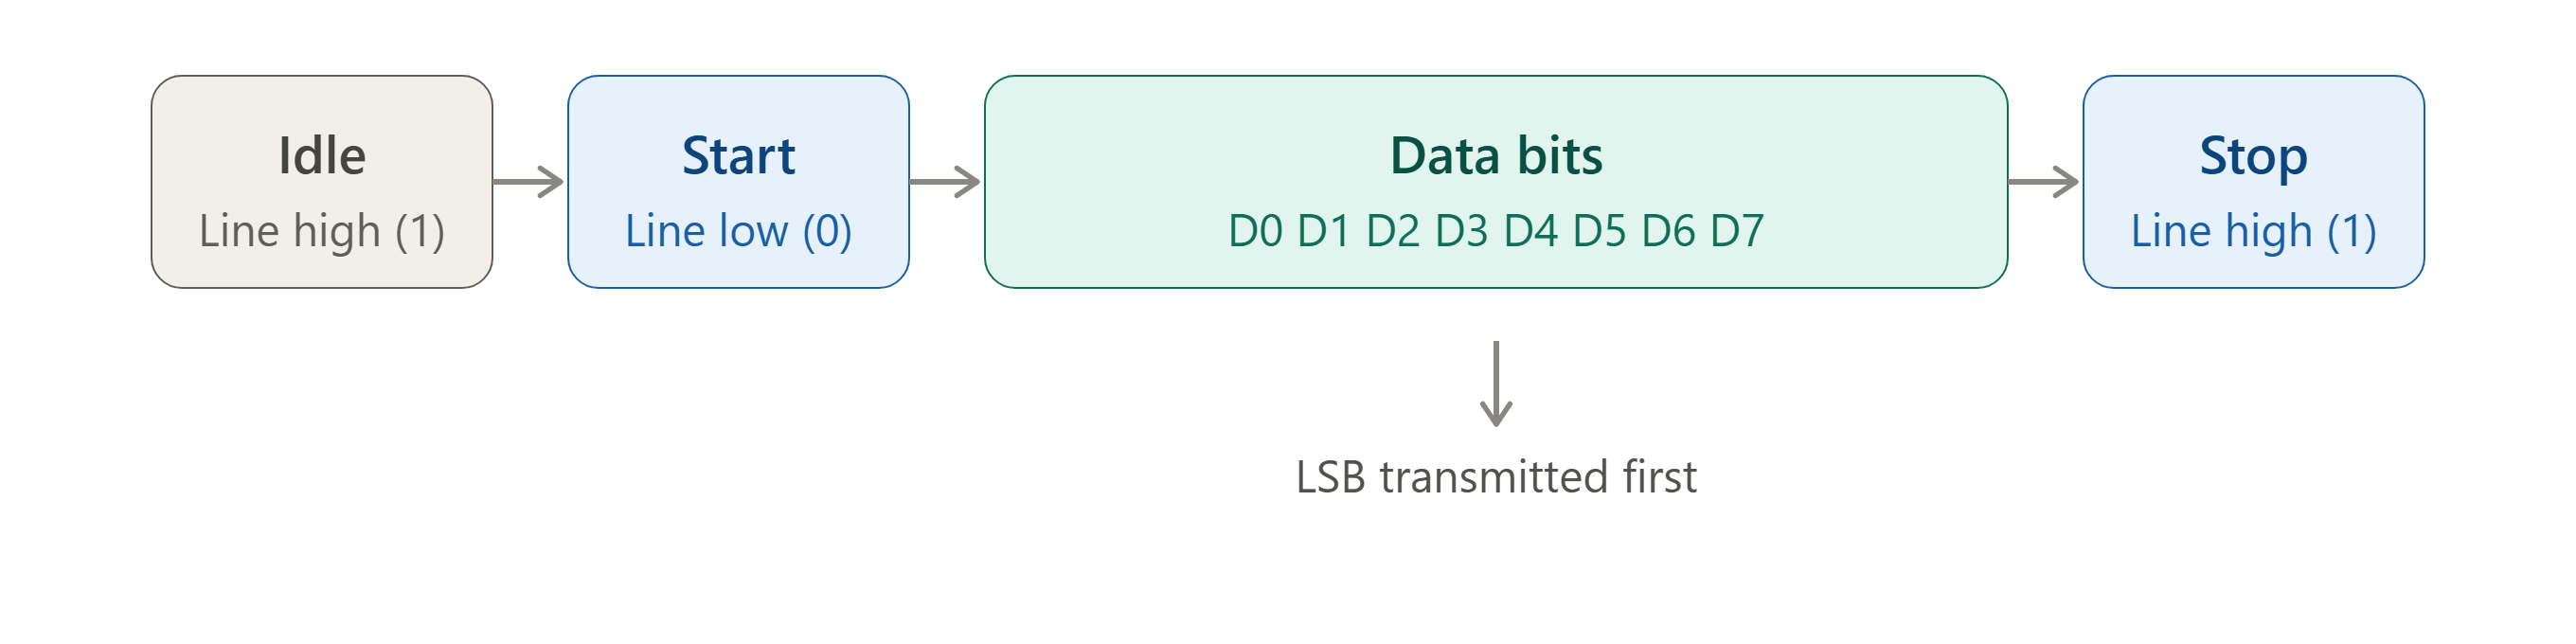
\includegraphics[width=0.90\linewidth]{images/uart_frame_flowchart.png}
    \caption{Standard UART Communication Frame.}
    \label{fig:uart_frame}
\end{figure}

Figure~\ref{fig:uart_frame} illustrates the structure of a standard UART data frame. Communication begins with a start bit followed by the data bits, an optional parity bit, and one or more stop bits. This frame structure enables asynchronous communication without requiring a dedicated clock signal between communicating devices.

%==========================================================

\section{Applications of UART}

Because of its simplicity and reliability, UART is widely employed in both academic and industrial electronic systems. Some common applications include:

\begin{itemize}

\item Embedded systems and microcontrollers

\item FPGA and ASIC-based digital systems

\item Sensor interfacing

\item GPS and Bluetooth communication modules

\item Industrial automation and control systems

\item Internet of Things (IoT) devices

\item Debugging and serial terminal communication

\item System-on-Chip (SoC) communication interfaces

\end{itemize}

The widespread adoption of UART makes it one of the most important communication peripherals in digital integrated circuits. Consequently, implementing a UART Transceiver IP Core using a complete RTL-to-GDSII ASIC design flow provides valuable practical experience in modern digital VLSI design methodologies.

\clearpage

%==========================================================

\section{Project Overview}

This project focuses on the complete RTL-to-GDSII implementation of 
a UART Transceiver IP Core using the OpenLane2 open-source ASIC design flow. The UART transceiver was designed in Verilog HDL and functionally verified using Verilator before proceeding through the complete physical implementation flow.

The implementation includes RTL design, functional verification, logic synthesis, floorplanning, power distribution network generation, placement, clock tree synthesis (CTS), global and detailed routing, parasitic extraction, static timing analysis (STA), IR-drop analysis, Design Rule Checking (DRC), Layout Versus Schematic (LVS) verification, and final GDSII layout generation. Throughout the implementation, reports generated at each stage were analyzed to evaluate design quality, area utilization, routing efficiency, timing performance, and manufacturability.

The project demonstrates how an RTL design is transformed into a fabrication-ready integrated circuit using an entirely open-source ASIC design environment based on the SkyWater SKY130A Process Design Kit (PDK).

%==========================================================

\section{Motivation}

Open-source Electronic Design Automation (EDA) tools have significantly simplified digital ASIC design by providing accessible alternatives to proprietary software. OpenLane2 integrates multiple open-source tools into a complete RTL-to-GDSII flow, enabling designers and students to gain practical experience in modern ASIC implementation.

The motivation behind this project is to understand every stage of the digital ASIC design flow by implementing a real communication IP core. Instead of limiting the work to RTL simulation, this project emphasizes complete physical implementation, report analysis, timing closure, routing optimization, physical verification, and manufacturability assessment.

%==========================================================

\section{Objectives}

The primary objectives of this project are:

\begin{itemize}

\item Design a synthesizable UART Transceiver IP Core using Verilog HDL.

\item Perform functional verification using Verilator.

\item Implement the complete RTL-to-GDSII ASIC flow using OpenLane2.

\item Analyze synthesis, placement, routing, timing, and utilization reports.

\item Perform RC extraction, IR-drop analysis, and static timing analysis.

\item Verify the final layout using Magic DRC, KLayout DRC, and Netgen LVS.

\item Generate a manufacturable GDSII layout.

\end{itemize}

%==========================================================

\section{Design Specifications}

Table~\ref{tab:design_specifications} summarizes the design environment and implementation specifications used throughout this project.

\begin{table}[!htbp]
\centering
\caption{Design Specifications}
\label{tab:design_specifications}

\renewcommand{\arraystretch}{1.3}

\begin{tabular}{|p{6cm}|p{7cm}|}
\hline

\textbf{Parameter} & \textbf{Specification} \\

\hline

Design & UART Transceiver IP Core \\

\hline

Hardware Description Language & Verilog HDL \\

\hline

Technology Node & 130 nm CMOS \\

\hline

Process Design Kit & SKY130A PDK \\

\hline

ASIC Flow & OpenLane2 \\

\hline

RTL Verification & Verilator \\

\hline

Logic Synthesis & Yosys \\

\hline

Physical Design & OpenROAD \\

\hline

Physical Verification & Magic, KLayout, Netgen \\

\hline

Operating System & Ubuntu 24.04 (WSL2) \\

\hline

Final Output & GDSII Layout \\

\hline

\end{tabular}

\end{table}

%==========================================================

\section{Project Methodology}

The complete implementation follows a standard digital ASIC design methodology beginning with RTL design and ending with GDSII generation. Each implementation stage produces reports that are analyzed to evaluate timing performance, silicon area, routing quality, power integrity, and physical correctness.

\begin{figure}[!htbp]
    \centering
    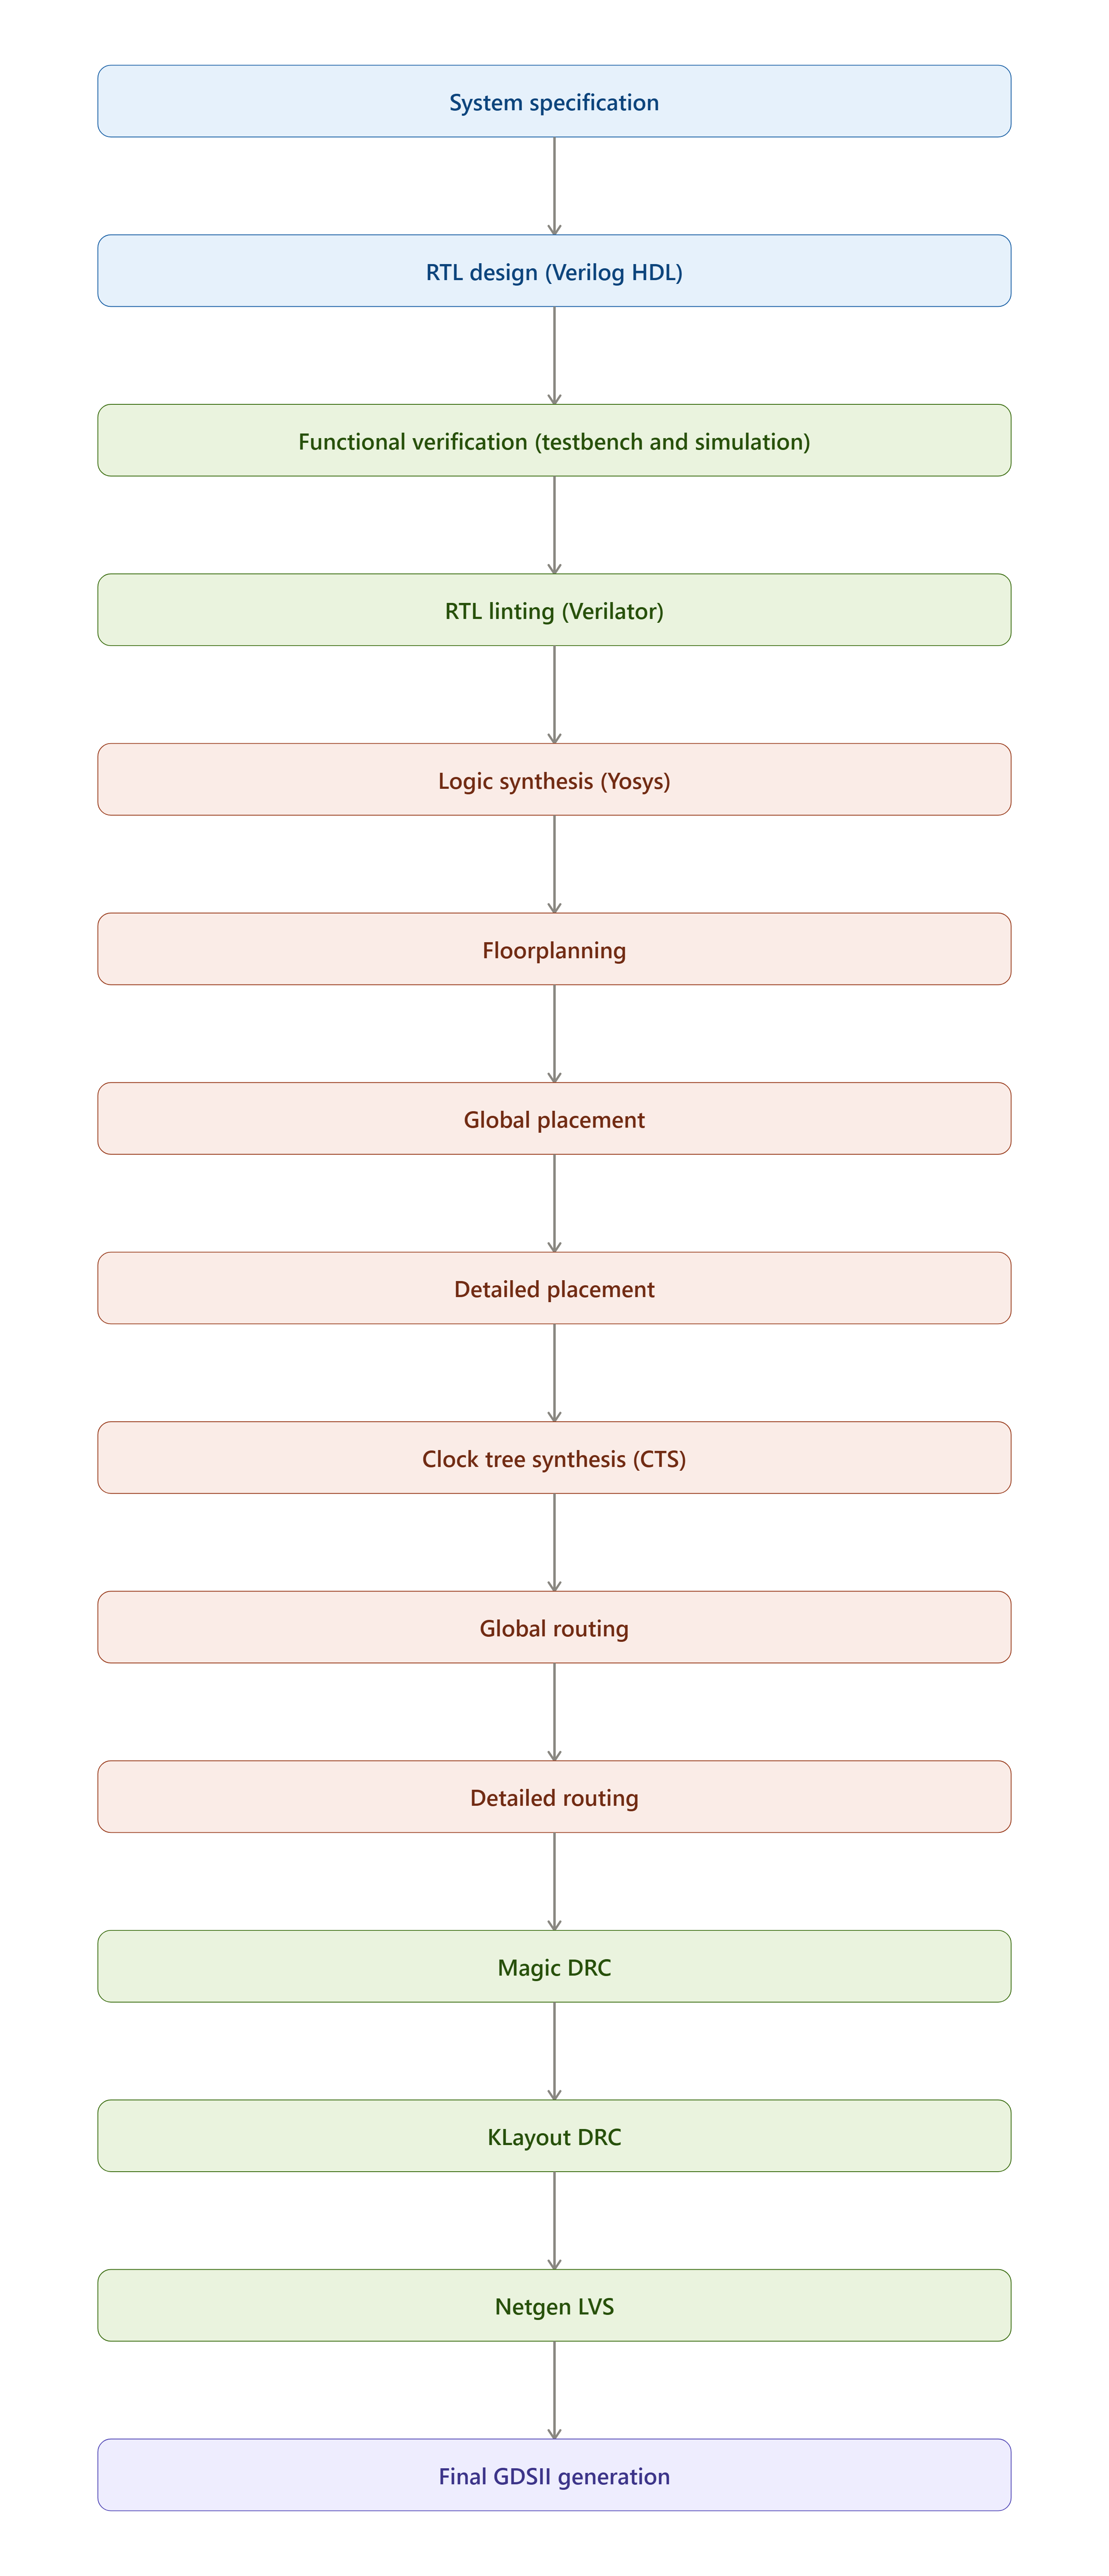
\includegraphics[width=0.92\linewidth]{images/asic_design_flow_full.png}
    \caption{Complete RTL-to-GDSII ASIC Design Flow adopted in this project.}
    \label{fig:asic_design_flow}
\end{figure}

As illustrated in Figure~\ref{fig:asic_design_flow}, the implementation begins with RTL development and functional verification, followed by logic synthesis, floorplanning, placement, clock tree synthesis, routing, RC extraction, static timing analysis, physical verification, and final GDSII layout generation. Each stage contributes to the successful realization of a fabrication-ready UART Transceiver ASIC.

The subsequent chapters discuss each implementation stage in detail, including the UART architecture, RTL implementation, verification methodology, physical design, report analysis, and signoff verification.

\clearpage
\chapter{System Architecture}

\section{UART Transceiver Architecture}

The UART Transceiver developed in this project is a modular digital design consisting of four major functional blocks: the UART Top module, Baud Rate Generator, UART Transmitter, and UART Receiver. The UART Top module integrates all submodules and controls the flow of data between the transmitter and receiver while sharing a common baud clock generated by the Baud Rate Generator.

The modular architecture improves design readability, simplifies verification, and allows individual modules to be synthesized and tested independently before integration. Such a hierarchical design methodology is commonly adopted in modern ASIC design to improve scalability and reusability.

\begin{figure}[!htbp]
    \centering
    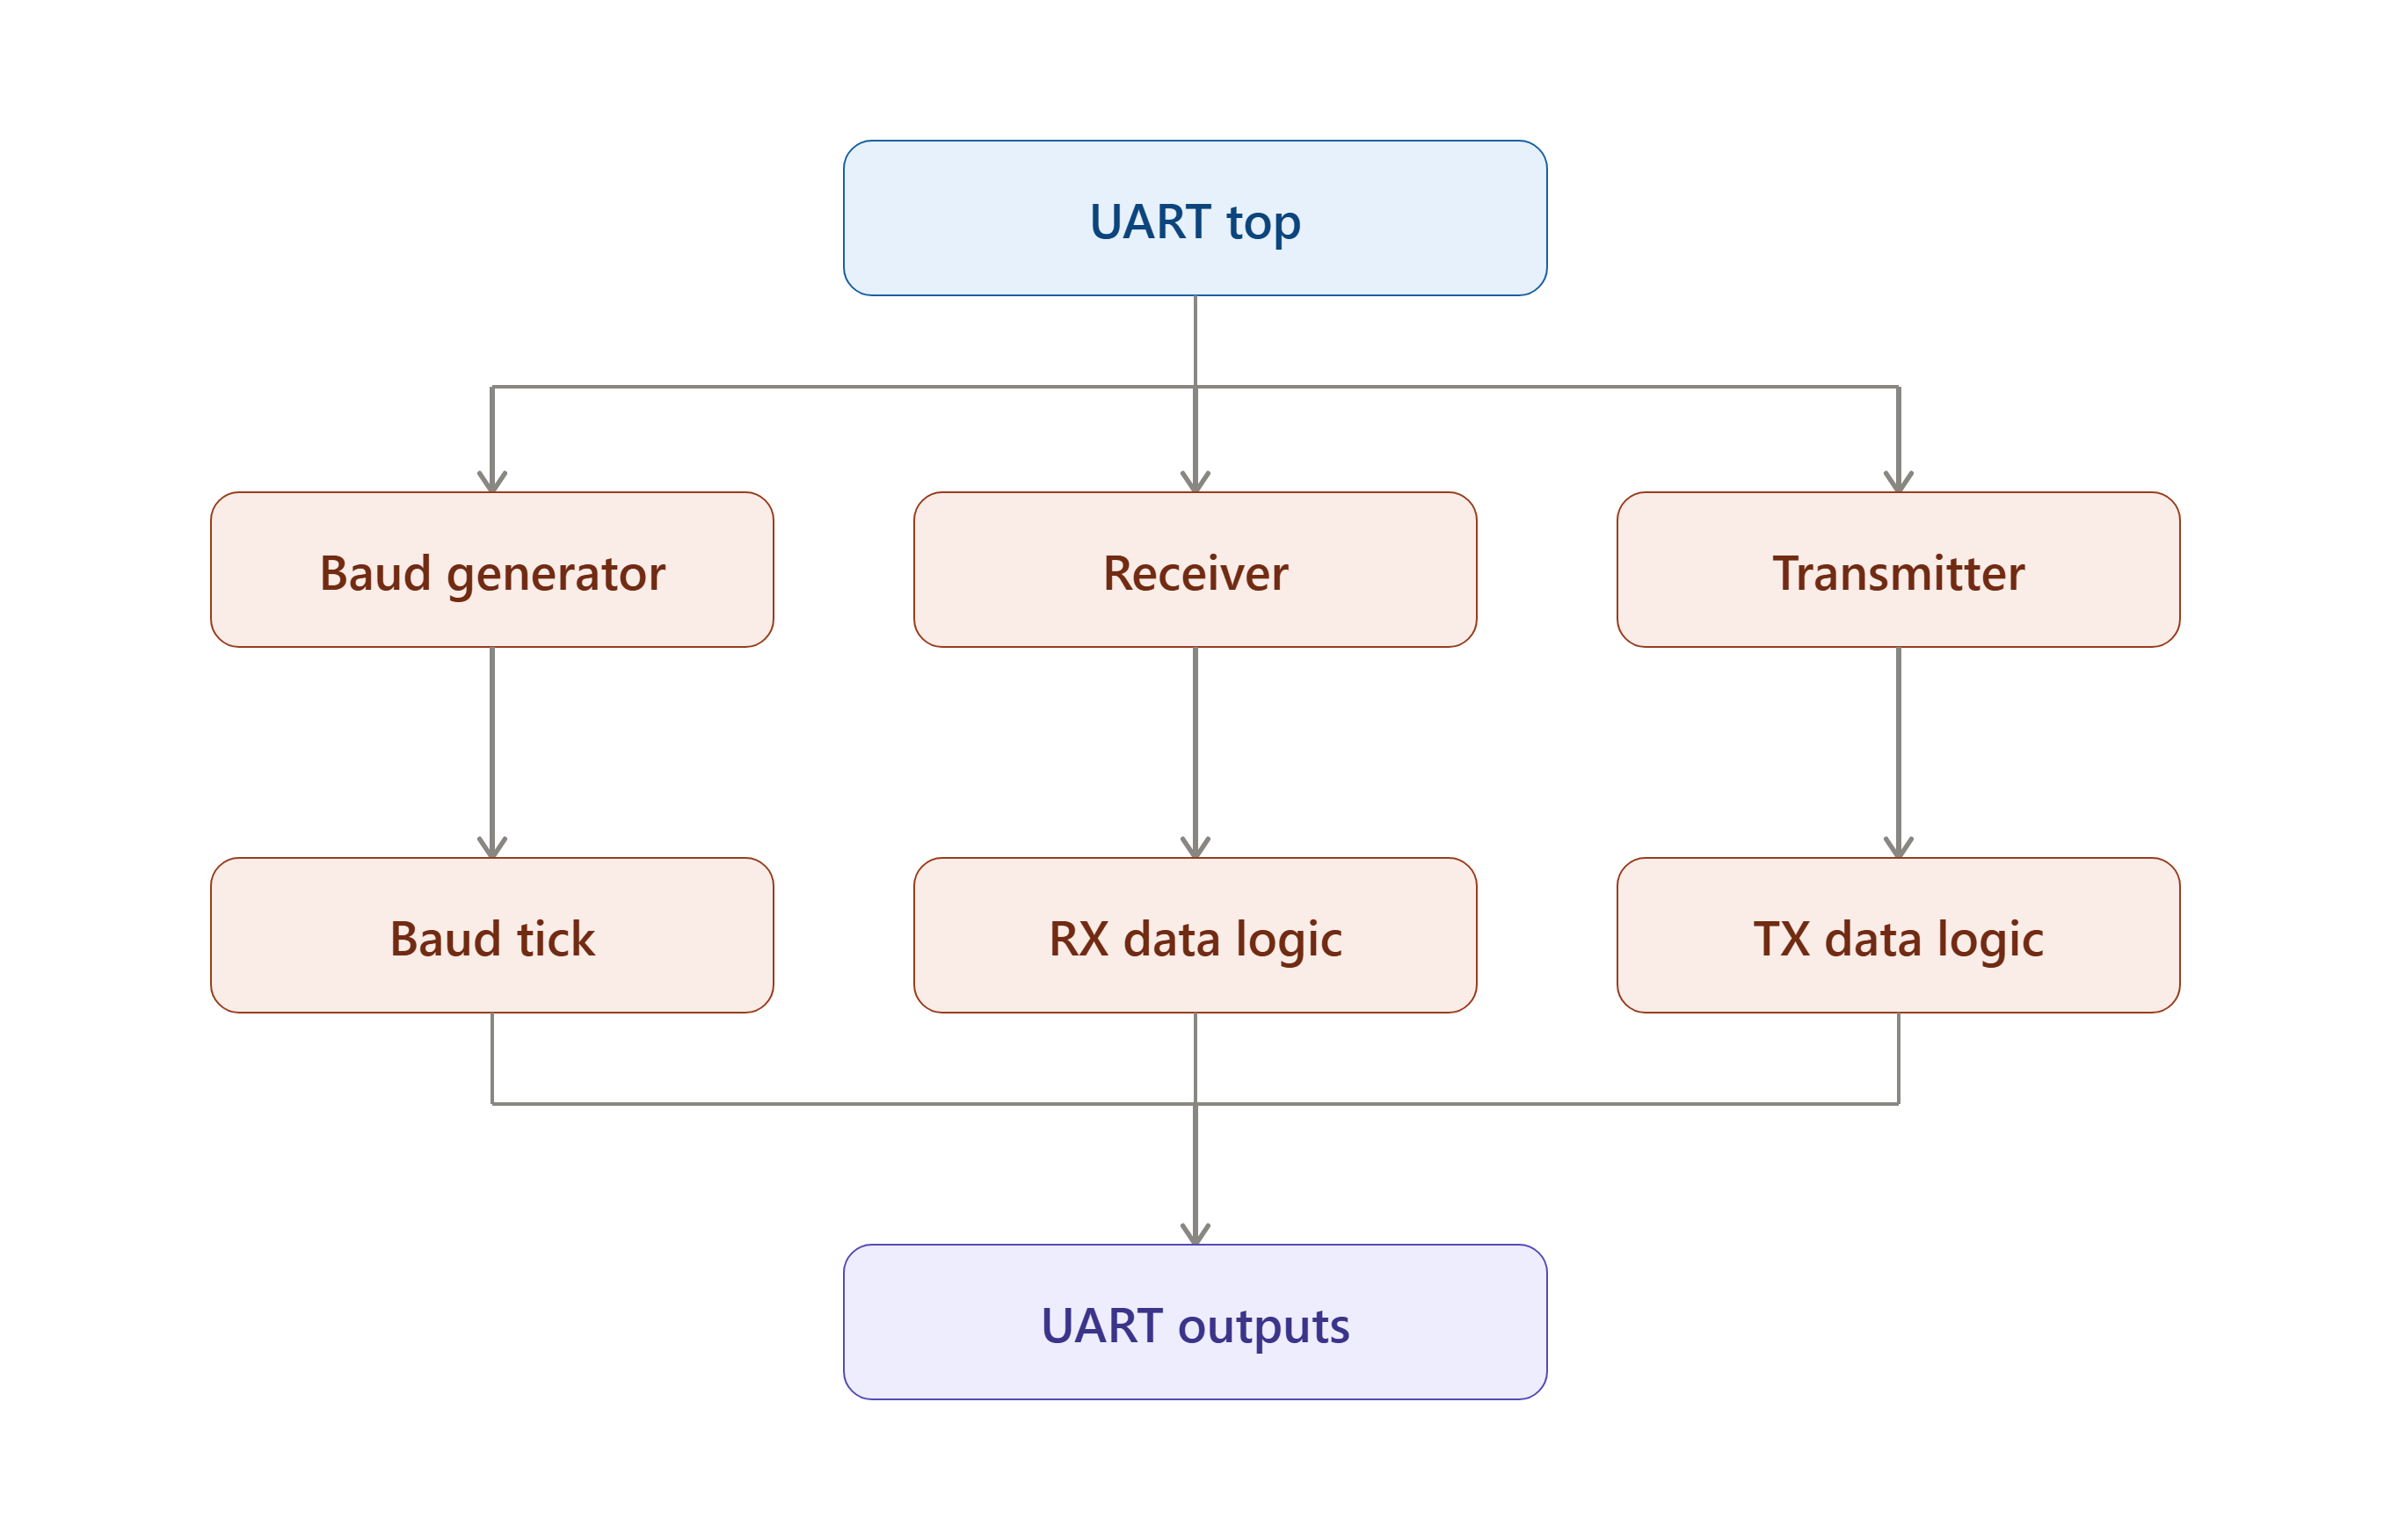
\includegraphics[width=0.88\linewidth]{images/uart_design_architecture.png}
    \caption{Top-Level Architecture of the UART Transceiver.}
    \label{fig:uart_top_architecture}
\end{figure}

Figure~\ref{fig:uart_top_architecture} illustrates the top-level organization of the UART Transceiver. The transmitter and receiver communicate through independent serial communication paths while both modules operate using the baud clock generated by the Baud Rate Generator.

%========================================================

\section{Internal Architecture}

Figure~\ref{fig:uart_internal_architecture} presents the complete internal architecture of the implemented UART Transceiver. The design consists of interconnected functional modules responsible for baud generation, serial transmission, serial reception, and top-level control.

\begin{figure}[!htbp]
    \centering
    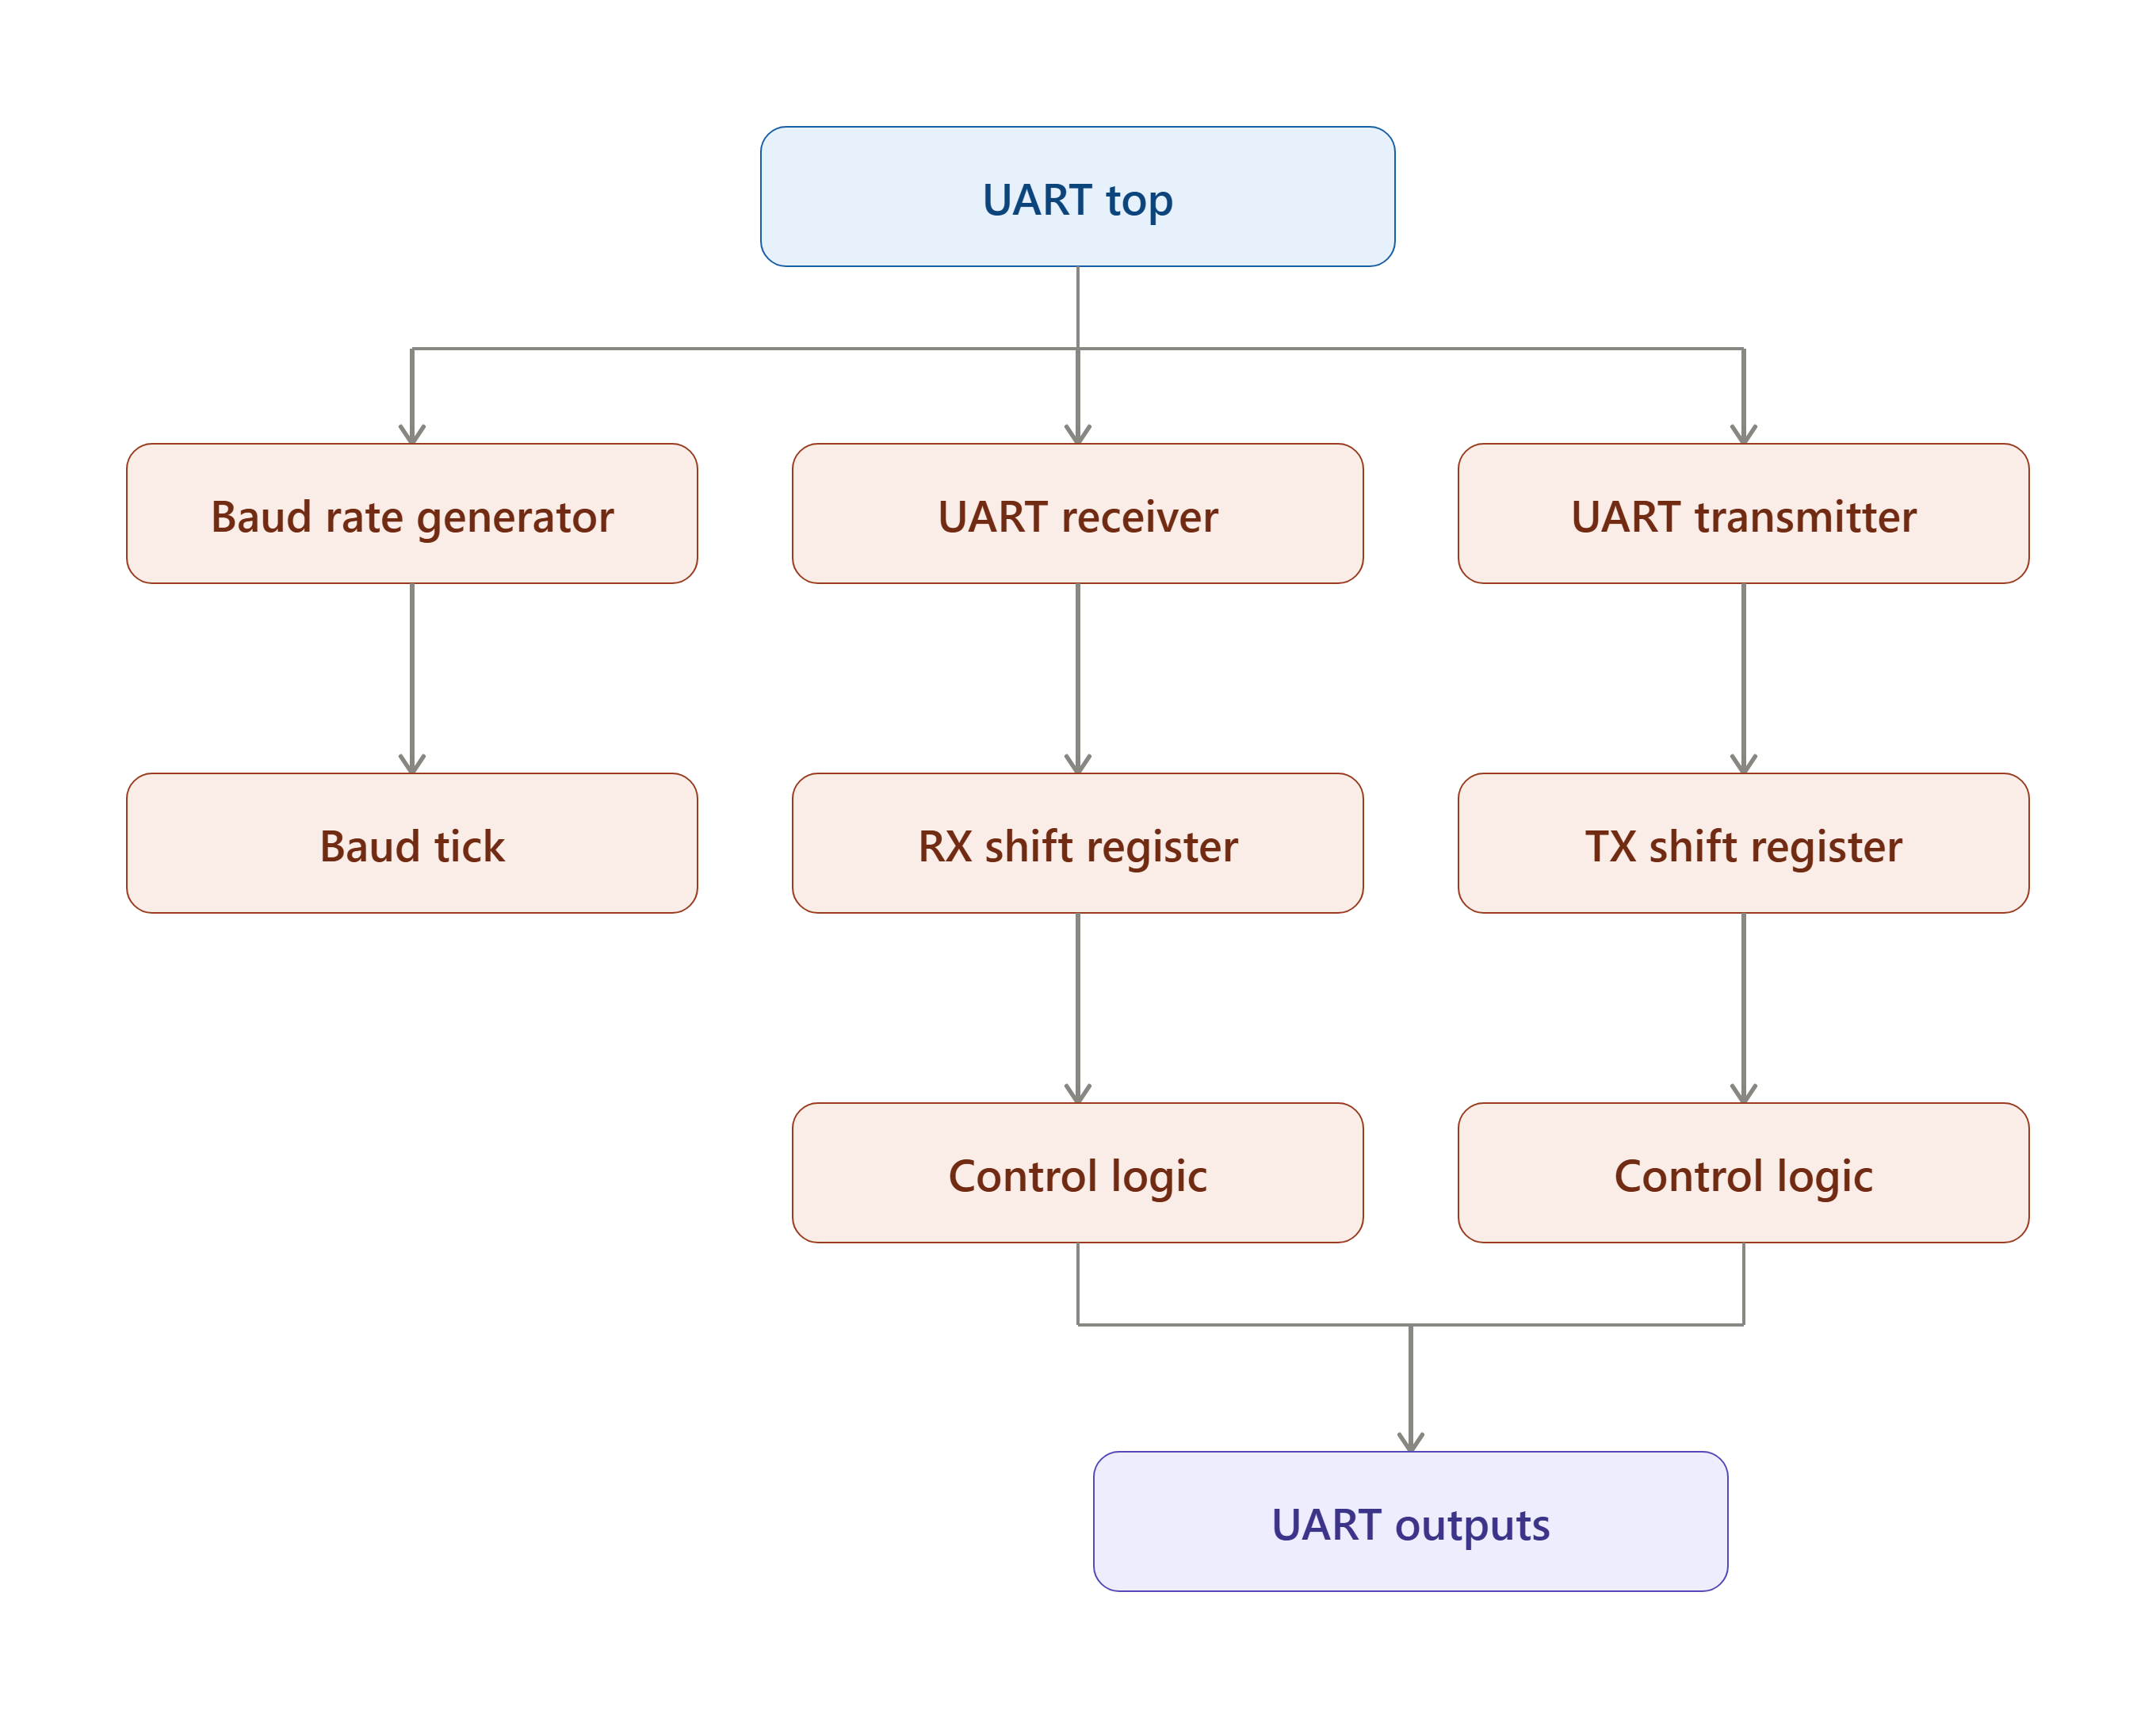
\includegraphics[width=0.92\linewidth]{images/complete_uart_internal_architecture.png}
    \caption{Internal Architecture of the UART Transceiver.}
    \label{fig:uart_internal_architecture}
\end{figure}

The hierarchical organization enables each module to perform a dedicated function while maintaining synchronized communication throughout the design. This approach simplifies debugging, verification, and future design modifications.

%========================================================

\section{Module Description}

Table~\ref{tab:uart_modules} summarizes the functionality of each major module implemented in the UART Transceiver.

\begin{table}[!htbp]
\centering
\caption{Functional Description of UART Modules}
\label{tab:uart_modules}

\renewcommand{\arraystretch}{1.3}

\begin{tabular}{|p{4cm}|p{9cm}|}

\hline

\textbf{Module} & \textbf{Function} \\

\hline

UART Top &
Integrates all functional modules and manages overall communication. \\

\hline

Baud Rate Generator &
Generates baud clock pulses from the system clock for synchronized data transmission and reception. \\

\hline

UART Transmitter &
Converts parallel input data into serial format according to the UART communication protocol. \\

\hline

UART Receiver &
Receives serial data and reconstructs the original parallel data while validating the received frame. \\

\hline

\end{tabular}

\end{table}

The following sections describe the architecture and operation of each module in detail.

%========================================================

\section{Baud Rate Generator}

The Baud Rate Generator is responsible for producing the baud clock required by both the UART transmitter and receiver. It divides the high-frequency system clock to generate timing pulses corresponding to the selected baud rate. Since both communication modules operate using the same baud timing, accurate baud generation is essential for reliable serial communication.

\begin{figure}[!htbp]
    \centering
    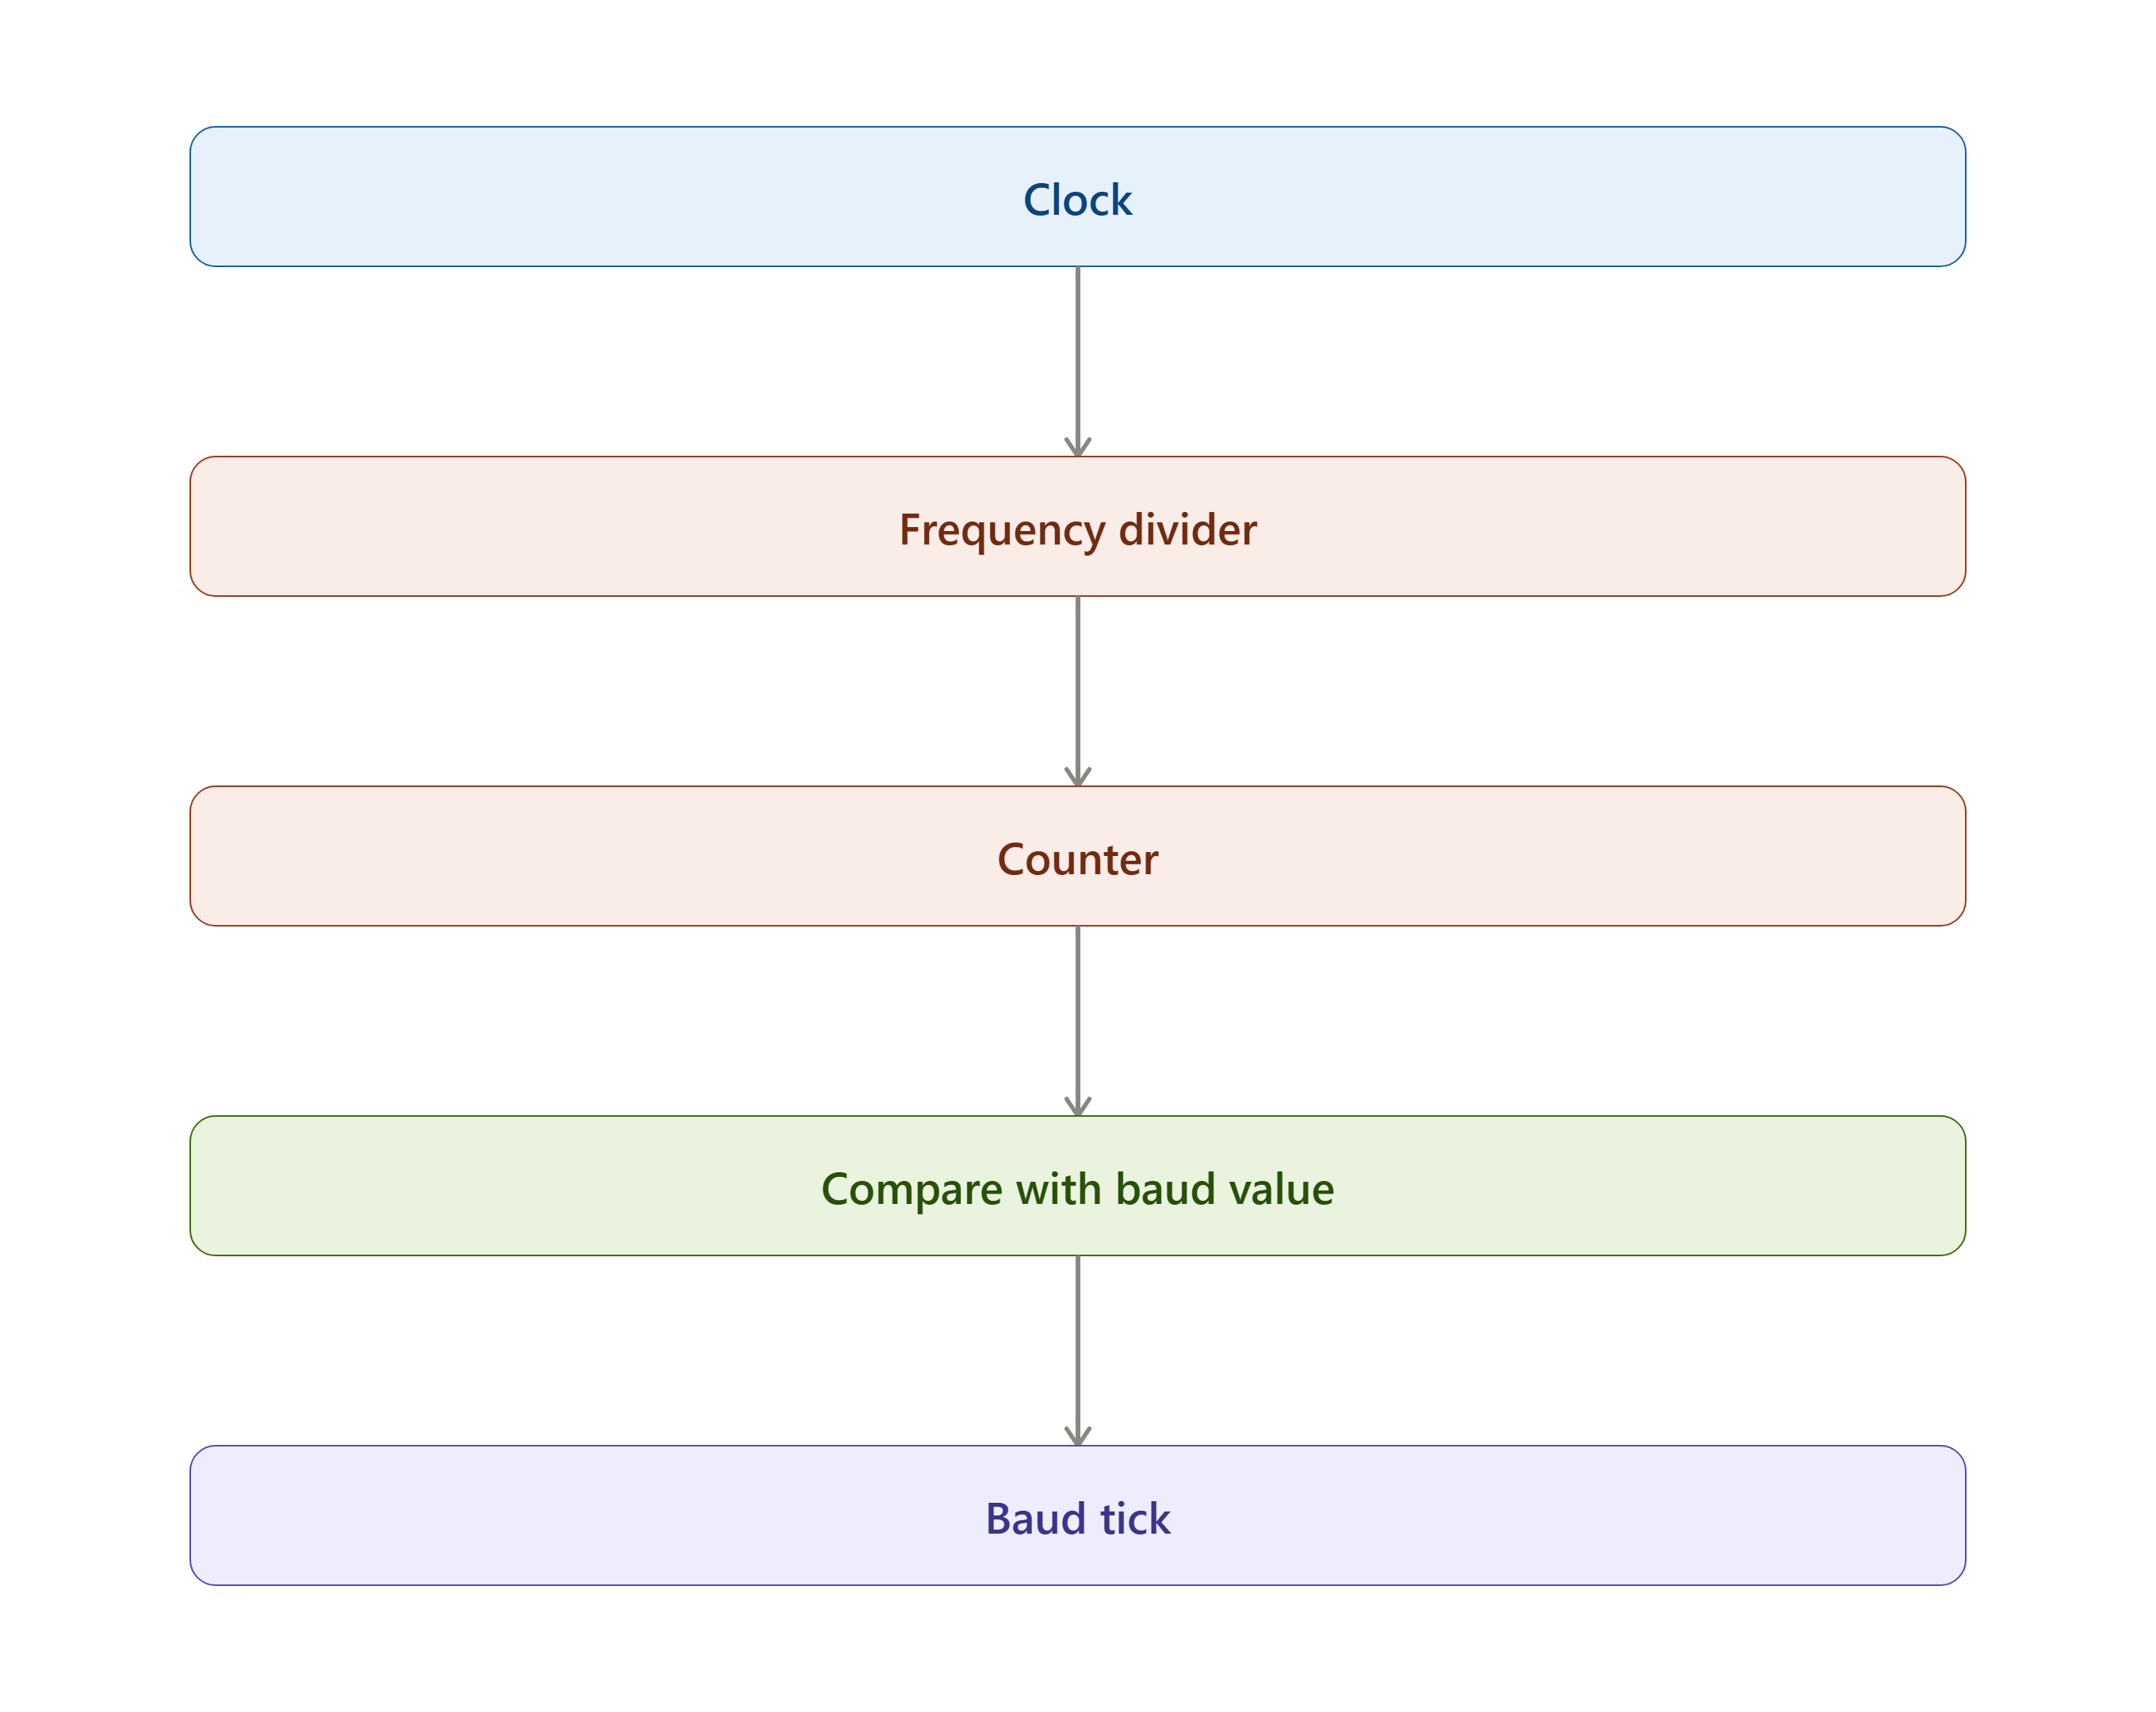
\includegraphics[width=0.80\linewidth]{images/baud_rate_generator_architecture.png}
    \caption{Architecture of the Baud Rate Generator.}
    \label{fig:baud_generator}
\end{figure}

The generated baud clock is distributed to both transmitter and receiver modules, ensuring synchronized operation throughout the communication process.

\clearpage

%========================================================

\section{UART Transmitter}

The UART Transmitter converts 8-bit parallel input data into a serial bit stream according to the UART communication protocol. Transmission begins only when the \texttt{tx\_start} control signal is asserted. The transmitter first sends the start bit, followed by the data bits in Least Significant Bit (LSB) first order, and finally transmits the stop bit to complete the communication frame.

The transmitter operates synchronously with the baud clock generated by the Baud Rate Generator, ensuring accurate timing for every transmitted bit.

\begin{figure}[!htbp]
    \centering
    \includegraphics[width=0.90\linewidth]{UART_Transmitter_Architecture}
    \caption{Architecture of the UART Transmitter.}
    \label{fig:uart_tx_architecture}
\end{figure}

Figure~\ref{fig:uart_tx_architecture} illustrates the internal organization of the transmitter module. The transmitter consists of control logic, shift registers, baud clock synchronization, and output logic that serializes the input data according to the UART protocol.

\vspace{0.3cm}

The major functions performed by the transmitter are:

\begin{itemize}

\item Accept 8-bit parallel input data.

\item Wait for the transmission enable signal.

\item Generate the start bit.

\item Shift data serially in LSB-first order.

\item Generate the stop bit.

\item Indicate transmission completion.

\end{itemize}

%========================================================

\subsection{Finite State Machine of UART Transmitter}

The transmitter operation is controlled by a Finite State Machine (FSM), which ensures that each communication frame follows the UART protocol correctly. The FSM sequentially controls the transmission of the start bit, data bits, and stop bit while maintaining synchronization with the baud clock.

\begin{figure}[!htbp]
\centering

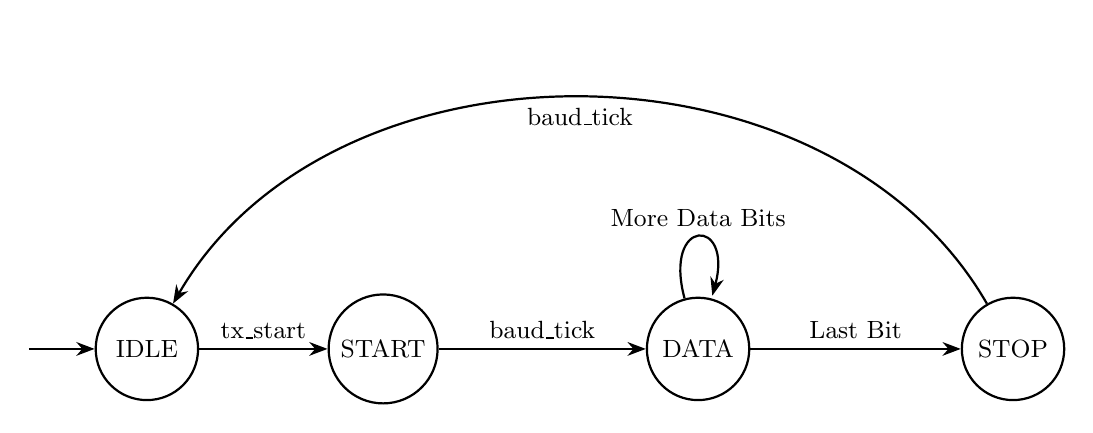
\begin{tikzpicture}[
>=Stealth,
every node/.style={font=\small},
state/.style={circle,draw,thick,minimum size=1.3cm}
]

% States
\node[state] (idle) at (0,0) {IDLE};
\node[state] (start) at (3,0) {START};
\node[state] (data) at (7,0) {DATA};
\node[state] (stop) at (11,0) {STOP};

% Initial Arrow
\draw[->,thick] (-1.5,0) -- (idle);

% State Transitions
\draw[->,thick] (idle) -- node[above]{tx\_start} (start);

\draw[->,thick] (start) -- node[above]{baud\_tick} (data);

\draw[->,thick]
(data) edge[loop above]
node{More Data Bits} ();

\draw[->,thick] (data) -- node[above]{Last Bit} (stop);

\draw[->,thick,bend right=60]
(stop) to node[below]{baud\_tick} (idle);

\end{tikzpicture}

\caption{Finite State Machine of the UART Transmitter.}
\label{fig:tx_fsm}

\end{figure}

The transmitter FSM consists of the following operating states:

\begin{itemize}

\item \textbf{Idle} – Waits for the transmission request.

\item \textbf{Start} – Sends the start bit.

\item \textbf{Data} – Serially transmits the 8-bit data.

\item \textbf{Stop} – Sends the stop bit and returns to the Idle state.

\end{itemize}

The FSM guarantees that every transmitted frame follows the required UART timing and frame structure.

%========================================================

\section{UART Receiver}

The UART Receiver performs the reverse operation of the transmitter by converting incoming serial data into an 8-bit parallel output. The receiver continuously monitors the RX line and begins reception after detecting the falling edge of the start bit. Data bits are sampled according to the baud clock and reconstructed into the original parallel data.

Once all bits are successfully received, the receiver validates the stop bit before asserting the \texttt{rx\_done} signal to indicate successful reception.

\begin{figure}[!htbp]
\centering

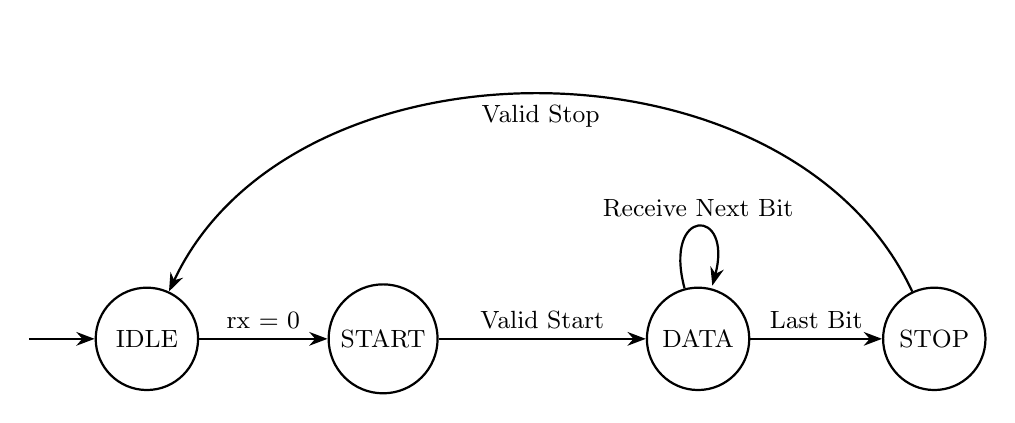
\begin{tikzpicture}[
>=Stealth,
every node/.style={font=\small},
state/.style={circle,draw,thick,minimum size=1.3cm}
]

% States
\node[state] (idle) at (0,0) {IDLE};
\node[state] (start) at (3,0) {START};
\node[state] (data) at (7,0) {DATA};
\node[state] (stop) at (10,0) {STOP};

% Initial Arrow
\draw[->,thick] (-1.5,0) -- (idle);

% State Transitions
\draw[->,thick] (idle) -- node[above]{rx = 0} (start);

\draw[->,thick] (start) -- node[above]{Valid Start} (data);

% DATA loop
\draw[->,thick]
(data) edge[loop above]
node{Receive Next Bit} ();

% DATA -> STOP
\draw[->,thick]
(data) -- node[above]{Last Bit} (stop);

% STOP -> IDLE
\draw[->,thick,bend right=65]
(stop) to node[below]{Valid Stop} (idle);

\end{tikzpicture}

\caption{Finite State Machine of the UART Receiver.}
\label{fig:rx_fsm}

\end{figure}


\vspace{0.3cm}

The receiver performs the following functions:

\begin{itemize}

\item Detect the incoming start bit.

\item Sample serial data using the baud clock.

\item Reconstruct the original 8-bit parallel data.

\item Verify the stop bit.

\item Assert the reception completion signal.

\end{itemize}

%========================================================

\subsection{Finite State Machine of UART Receiver}

Similar to the transmitter, the receiver operation is governed by a Finite State Machine (FSM). The FSM synchronizes data sampling with the baud clock and controls the complete reception process from start-bit detection to successful frame completion.

The receiver FSM consists of four primary states:

\begin{itemize}

\item \textbf{Idle} – Waits for the detection of the start bit.

\item \textbf{Start} – Confirms the validity of the detected start bit.

\item \textbf{Data} – Samples and stores the incoming serial bits.

\item \textbf{Stop} – Verifies the stop bit and completes the reception process.

\end{itemize}

This state-based implementation ensures reliable data reception while minimizing synchronization errors during asynchronous communication.

\clearpage

%========================================================

\section{Data Transmission and Reception Flow}

The operation of the UART Transceiver can be divided into two independent processes: data transmission and data reception. Although both modules operate independently, they are synchronized using the baud clock generated by the Baud Rate Generator. The following flowcharts illustrate the sequence of operations performed during transmission and reception.

%--------------------------------------------------------

\subsection{UART Transmission Flow}

The transmission process begins when valid parallel data and the transmission enable signal are applied to the UART Transmitter. The transmitter serializes the data by generating the start bit, transmitting the eight data bits, and finally appending the stop bit before returning to the idle state.

\begin{figure}[!htbp]
\centering

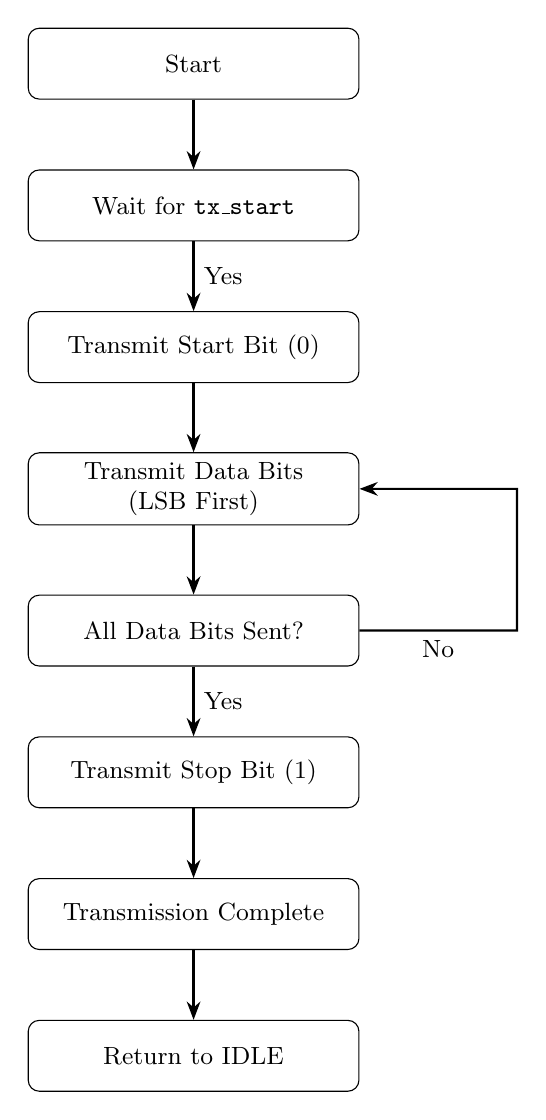
\begin{tikzpicture}[
>=Stealth,
every node/.style={font=\small},
block/.style={
draw,
rectangle,
rounded corners,
minimum width=4.2cm,
minimum height=0.9cm,
align=center
}
]

% Blocks
\node[block] (start) at (0,0) {Start};

\node[block] (wait) at (0,-1.8)
{Wait for \texttt{tx\_start}};

\node[block] (startbit) at (0,-3.6)
{Transmit Start Bit (0)};

\node[block] (data) at (0,-5.4)
{Transmit Data Bits\\(LSB First)};

\node[block] (check) at (0,-7.2)
{All Data Bits Sent?};

\node[block] (stop) at (0,-9.0)
{Transmit Stop Bit (1)};

\node[block] (done) at (0,-10.8)
{Transmission Complete};

\node[block] (idle) at (0,-12.6)
{Return to IDLE};

% Arrows
\draw[->,thick] (start) -- (wait);

\draw[->,thick] (wait) -- node[right]{Yes} (startbit);

\draw[->,thick] (startbit) -- (data);

\draw[->,thick] (data) -- (check);

\draw[->,thick] (check) -- node[right]{Yes} (stop);

\draw[->,thick] (stop) -- (done);

\draw[->,thick] (done) -- (idle);

% No branch
\draw[->,thick]
(check.east) -- ++(2,0)
node[midway,below]{No}
-- ++(0,1.8)
-- (data.east);

\end{tikzpicture}

\caption{Flowchart of UART Data Transmission.}
\label{fig:tx_flowchart}

\end{figure}

Figure~\ref{fig:tx_flowchart} shows the sequential execution of the transmission process. Each state transition is synchronized with the baud clock to ensure accurate serial data transmission.

%--------------------------------------------------------

\subsection{UART Reception Flow}

The receiver continuously monitors the RX line for the detection of a valid start bit. Once detected, the receiver samples the incoming serial data using the baud clock, reconstructs the original 8-bit parallel data, verifies the stop bit, and asserts the reception complete signal.

\begin{figure}[!htbp]
\centering

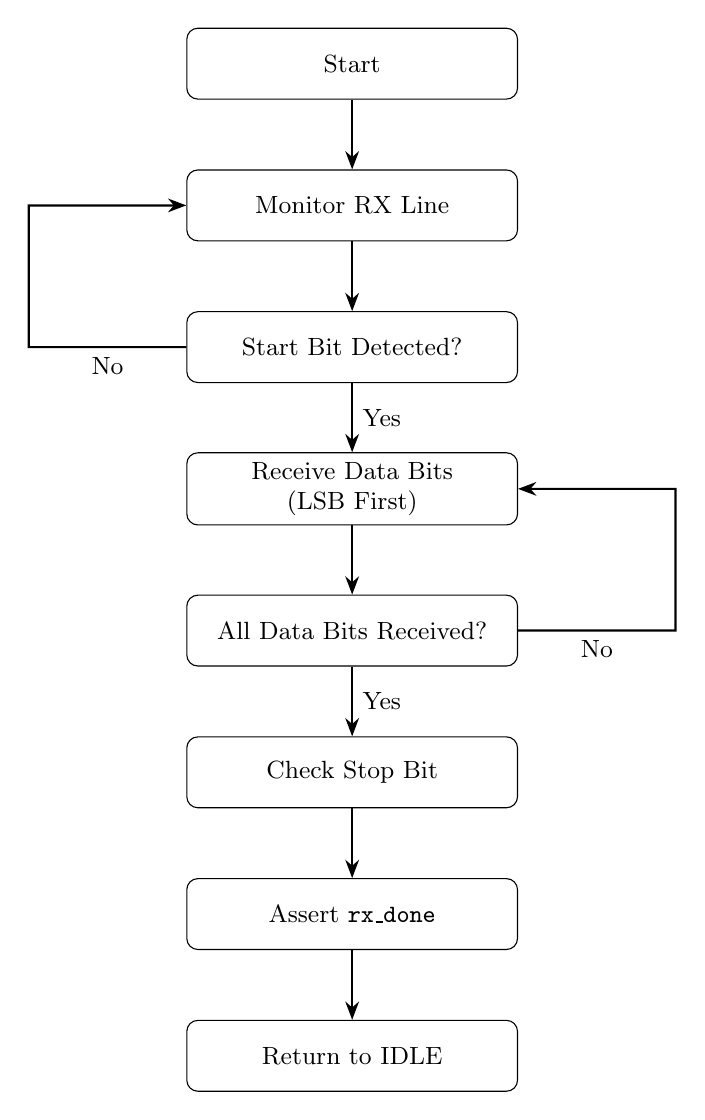
\begin{tikzpicture}[
>=Stealth,
every node/.style={font=\small},
block/.style={
draw,
rectangle,
rounded corners,
minimum width=4.2cm,
minimum height=0.9cm,
align=center
}
]

% Blocks
\node[block] (start) at (0,0) {Start};

\node[block] (monitor) at (0,-1.8)
{Monitor RX Line};

\node[block] (detect) at (0,-3.6)
{Start Bit Detected?};

\node[block] (receive) at (0,-5.4)
{Receive Data Bits\\(LSB First)};

\node[block] (check) at (0,-7.2)
{All Data Bits Received?};

\node[block] (stop) at (0,-9.0)
{Check Stop Bit};

\node[block] (done) at (0,-10.8)
{Assert \texttt{rx\_done}};

\node[block] (idle) at (0,-12.6)
{Return to IDLE};

% Arrows
\draw[->,thick] (start) -- (monitor);

\draw[->,thick] (monitor) -- (detect);

\draw[->,thick] (detect) -- node[right]{Yes} (receive);

\draw[->,thick] (receive) -- (check);

\draw[->,thick] (check) -- node[right]{Yes} (stop);

\draw[->,thick] (stop) -- (done);

\draw[->,thick] (done) -- (idle);

% No branch from Detect
\draw[->,thick]
(detect.west) -- ++(-2,0)
node[midway,below]{No}
-- ++(0,1.8)
-- (monitor.west);

% No branch from Check
\draw[->,thick]
(check.east) -- ++(2,0)
node[midway,below]{No}
-- ++(0,1.8)
-- (receive.east);

\end{tikzpicture}

\caption{Flowchart of UART Data Reception.}
\label{fig:rx_flowchart}

\end{figure}

Figure~\ref{fig:rx_flowchart} illustrates the sequence followed by the receiver to recover the transmitted data while maintaining synchronization with the communication frame.

%========================================================

\section{Top Module Integration}

The UART Top module integrates the Baud Rate Generator, UART Transmitter, and UART Receiver into a single functional IP core. It distributes the baud clock to both communication modules, accepts parallel input data for transmission, receives serial input data, and provides the reconstructed parallel output.

\begin{figure}[!htbp]
\centering

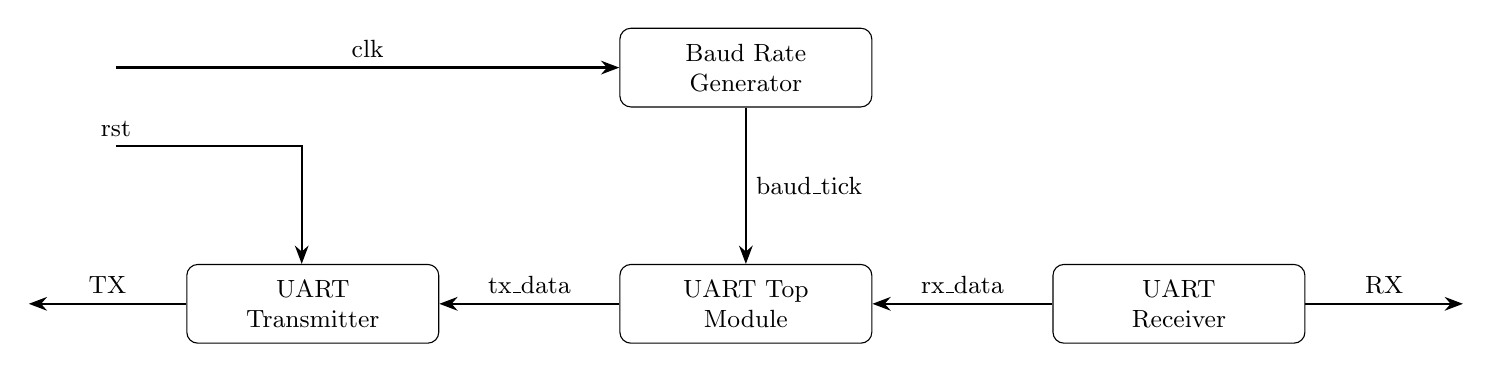
\begin{tikzpicture}[
>=Stealth,
every node/.style={font=\small},
block/.style={
draw,
rectangle,
rounded corners,
minimum width=3.2cm,
minimum height=1.0cm,
align=center
}
]

%-------------------------------------------------
% Blocks
%-------------------------------------------------

\node[block] (baud) at (0,3)
{Baud Rate\\Generator};

\node[block] (tx) at (-5.5,0)
{UART\\Transmitter};

\node[block] (top) at (0,0)
{UART Top\\Module};

\node[block] (rx) at (5.5,0)
{UART\\Receiver};

%-------------------------------------------------
% Clock
%-------------------------------------------------

\draw[->,thick]
(-8,3) -- node[above]{clk} (baud.west);

%-------------------------------------------------
% Baud Tick
%-------------------------------------------------

\draw[->,thick]
(baud.south) -- node[right]{baud\_tick} (top.north);

%-------------------------------------------------
% Reset
%-------------------------------------------------

\draw[->,thick]
(-8,2) node[above]{rst} -| ([xshift=-4pt]tx.north);

%-------------------------------------------------
% TX Path
%-------------------------------------------------

\draw[->,thick]
(top.west) -- node[above]{tx\_data} (tx.east);

\draw[->,thick]
(tx.west) -- ++(-2,0)
node[midway,above]{TX};

%-------------------------------------------------
% RX Path
%-------------------------------------------------

\draw[->,thick]
(rx.east) -- ++(2,0)
node[midway,above]{RX};

\draw[->,thick]
(rx.west) -- node[above]{rx\_data} (top.east);

\end{tikzpicture}

\caption{Block Diagram of the UART Top Module.}
\label{fig:uart_top_block}

\end{figure}

Figure~\ref{fig:uart_top_flow} illustrates the interaction between all major functional modules within the UART Transceiver. The top-level controller coordinates the complete communication process by connecting the baud generation, transmission, and reception blocks.

%========================================================
The architecture presented in this chapter forms the basis of the RTL implementation described in the next chapter. The following chapter discusses the Verilog HDL implementation of each module along with functional simulation and verification prior to ASIC synthesis.

\clearpage
\chapter{RTL Design and Verification}
\label{chap:rtl_design}

The UART IP core was developed using Verilog HDL following a modular design methodology. The complete RTL design consists of four independent modules: the Baud Rate Generator, UART Transmitter, UART Receiver, and the UART Top module. Each module was verified individually using dedicated testbenches before performing complete system-level verification.

The RTL implementation was written to be fully synthesizable and compatible with the SkyWater SKY130 standard cell library used by the OpenLane2 ASIC design flow.

\vspace{0.3cm}

The verification process consisted of individual module simulations followed by complete UART functionality testing.

%%%%%%%%%%%%%%%%%%%%%%%%%%%%%%%%%%%%%%%%%%%%%%%%%%%%%%%%%%%%

\section{RTL Module Organization}

The complete UART design is divided into four reusable RTL modules.

\begin{table}[!htbp]
\centering
\caption{UART RTL modules}
\label{tab:rtl_modules}
\begin{tabular}{ll}
\toprule
Module & Function\\
\midrule
Baud Generator & Generates baud tick from system clock\\
UART Transmitter & Converts parallel data into serial data\\
UART Receiver & Converts serial data into parallel data\\
UART Top & Integrates all UART modules\\
\bottomrule
\end{tabular}
\end{table}

The modular architecture improves readability, verification, scalability and future reuse of the IP.

%%%%%%%%%%%%%%%%%%%%%%%%%%%%%%%%%%%%%%%%%%%%%%%%%%%%%%%%%%%%

\section{Baud Rate Generator}

The baud rate generator produces a periodic \texttt{baud\_tick} signal required by both the transmitter and receiver. It divides the incoming system clock using a programmable counter so that data transmission occurs at the required baud rate.

\subsection*{Module Interface}

\begin{table}[!htbp]
\centering
\caption{Baud Generator ports}
\label{tab:baud_ports}
\begin{tabular}{llll}
\toprule
Signal & Direction & Width & Description\\
\midrule
clk & Input & 1 & System clock\\
rst & Input & 1 & Active-high reset\\
baud\_tick & Output & 1 & Baud timing pulse\\
\bottomrule
\end{tabular}
\end{table}

The RTL schematic generated by Yosys is shown below.

\begin{figure}[!htbp]
\centering
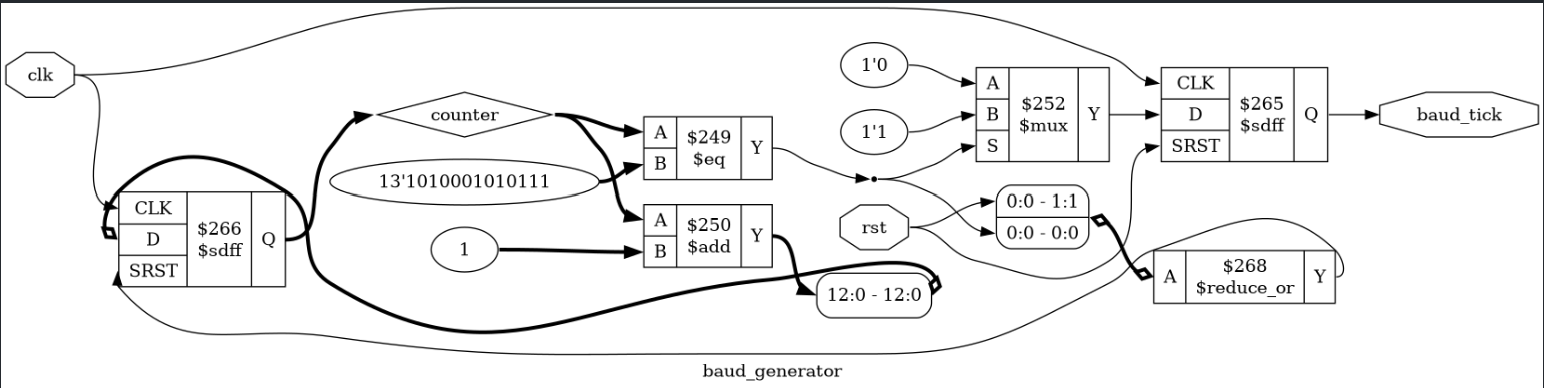
\includegraphics[width=\textwidth]{images/baud_generator_rtl.png}
\caption{RTL schematic of the Baud Rate Generator generated using Yosys.}
\label{fig:baud_rtl}
\end{figure}

%%%%%%%%%%%%%%%%%%%%%%%%%%%%%%%%%%%%%%%%%%%%%%%%%%%%%%%%%%%%

\section{UART Transmitter}

The transmitter converts an 8-bit parallel word into a serial UART frame consisting of a start bit, eight data bits and a stop bit. Data shifting is synchronized using the baud tick generated by the baud rate generator.


\subsection*{Module Interface}

\begin{table}[!htbp]
\centering
\caption{UART transmitter ports}
\label{tab:tx_ports}
\begin{tabular}{llll}
\toprule
Signal & Direction & Width & Description\\
\midrule
clk & Input & 1 & System clock\\
rst & Input & 1 & Reset\\
baud\_tick & Input & 1 & Baud timing pulse\\
tx\_start & Input & 1 & Transmission enable\\
tx\_data & Input & 8 & Parallel input data\\
tx & Output & 1 & Serial output\\
tx\_busy & Output & 1 & Busy flag\\
\bottomrule
\end{tabular}
\end{table}

\begin{figure}[!htbp]
\centering
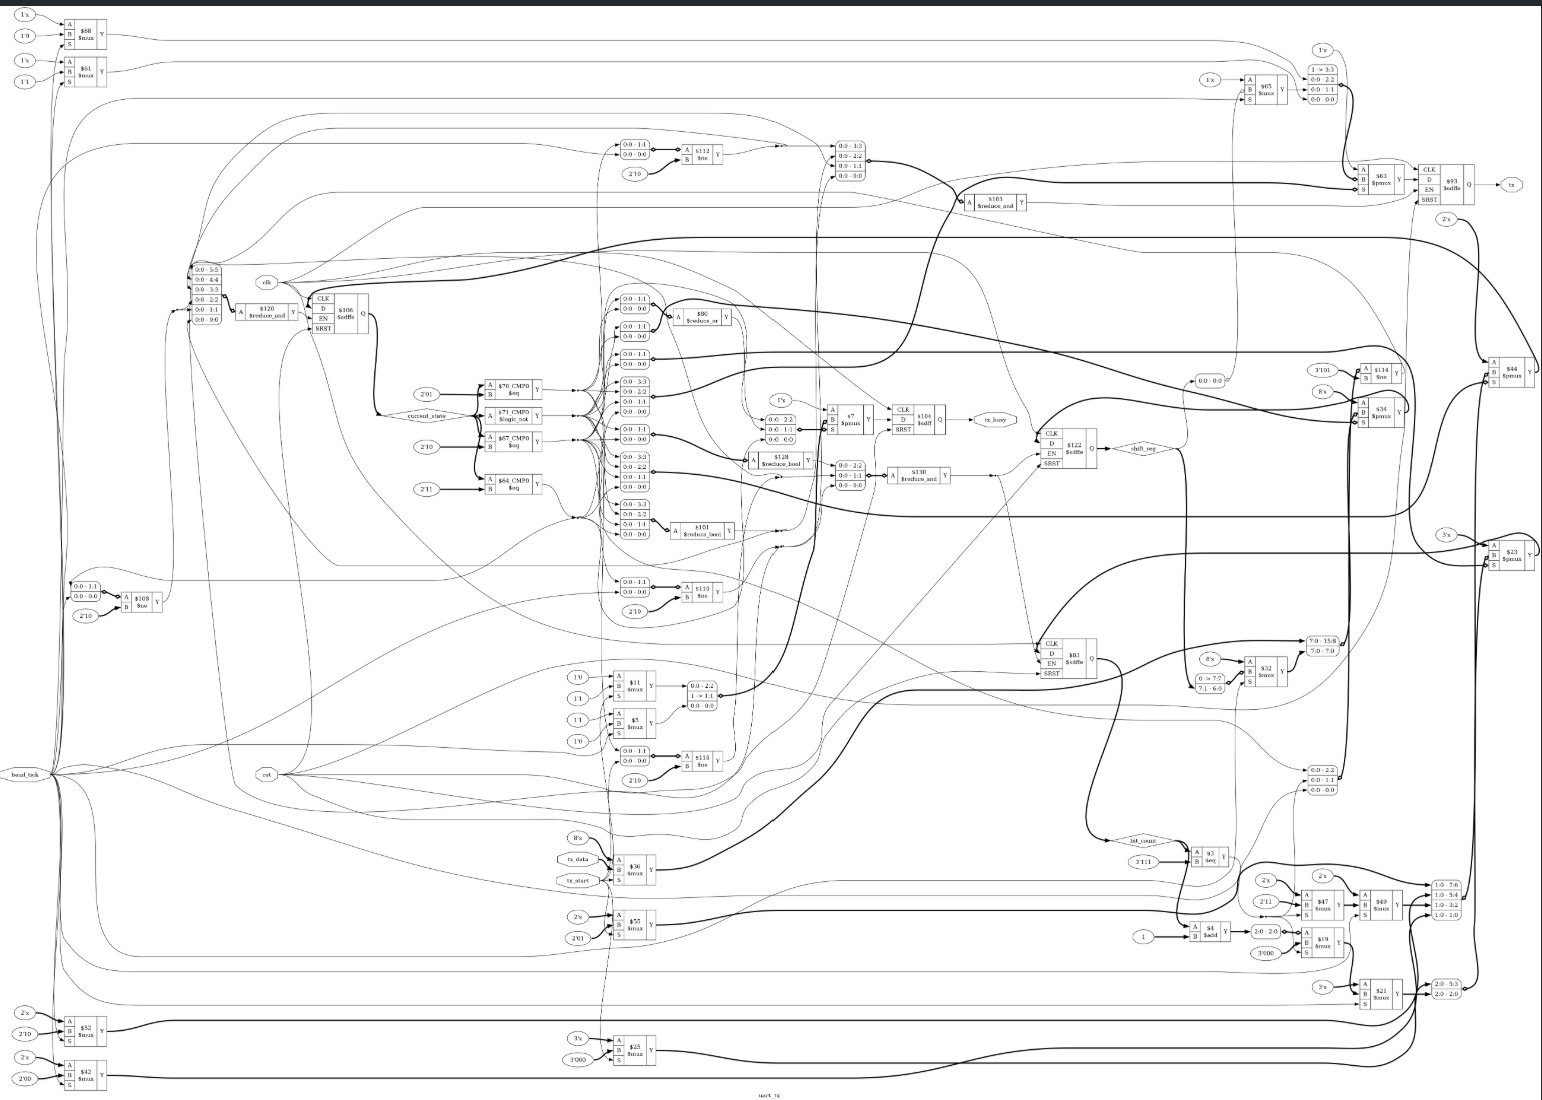
\includegraphics[width=\textwidth]{images/uart_tx_rtl.png}
\caption{RTL schematic of the UART transmitter generated using Yosys.}
\label{fig:tx_rtl}
\end{figure}

%%%%%%%%%%%%%%%%%%%%%%%%%%%%%%%%%%%%%%%%%%%%%%%%%%%%%%%%%%%%

\section{UART Receiver}

The receiver continuously monitors the RX line for a valid start bit. After detecting the start bit, it samples each incoming data bit at the baud rate and reconstructs the original 8-bit data word.


\subsection*{Module Interface}

\begin{table}[!htbp]
\centering
\caption{UART receiver ports}
\label{tab:rx_ports}
\begin{tabular}{llll}
\toprule
Signal & Direction & Width & Description\\
\midrule
clk & Input & 1 & System clock\\
rst & Input & 1 & Reset\\
baud\_tick & Input & 1 & Baud timing pulse\\
rx & Input & 1 & Serial input\\
rx\_data & Output & 8 & Received data\\
rx\_done & Output & 1 & Reception complete flag\\
\bottomrule
\end{tabular}
\end{table}

\begin{figure}[!htbp]
\centering
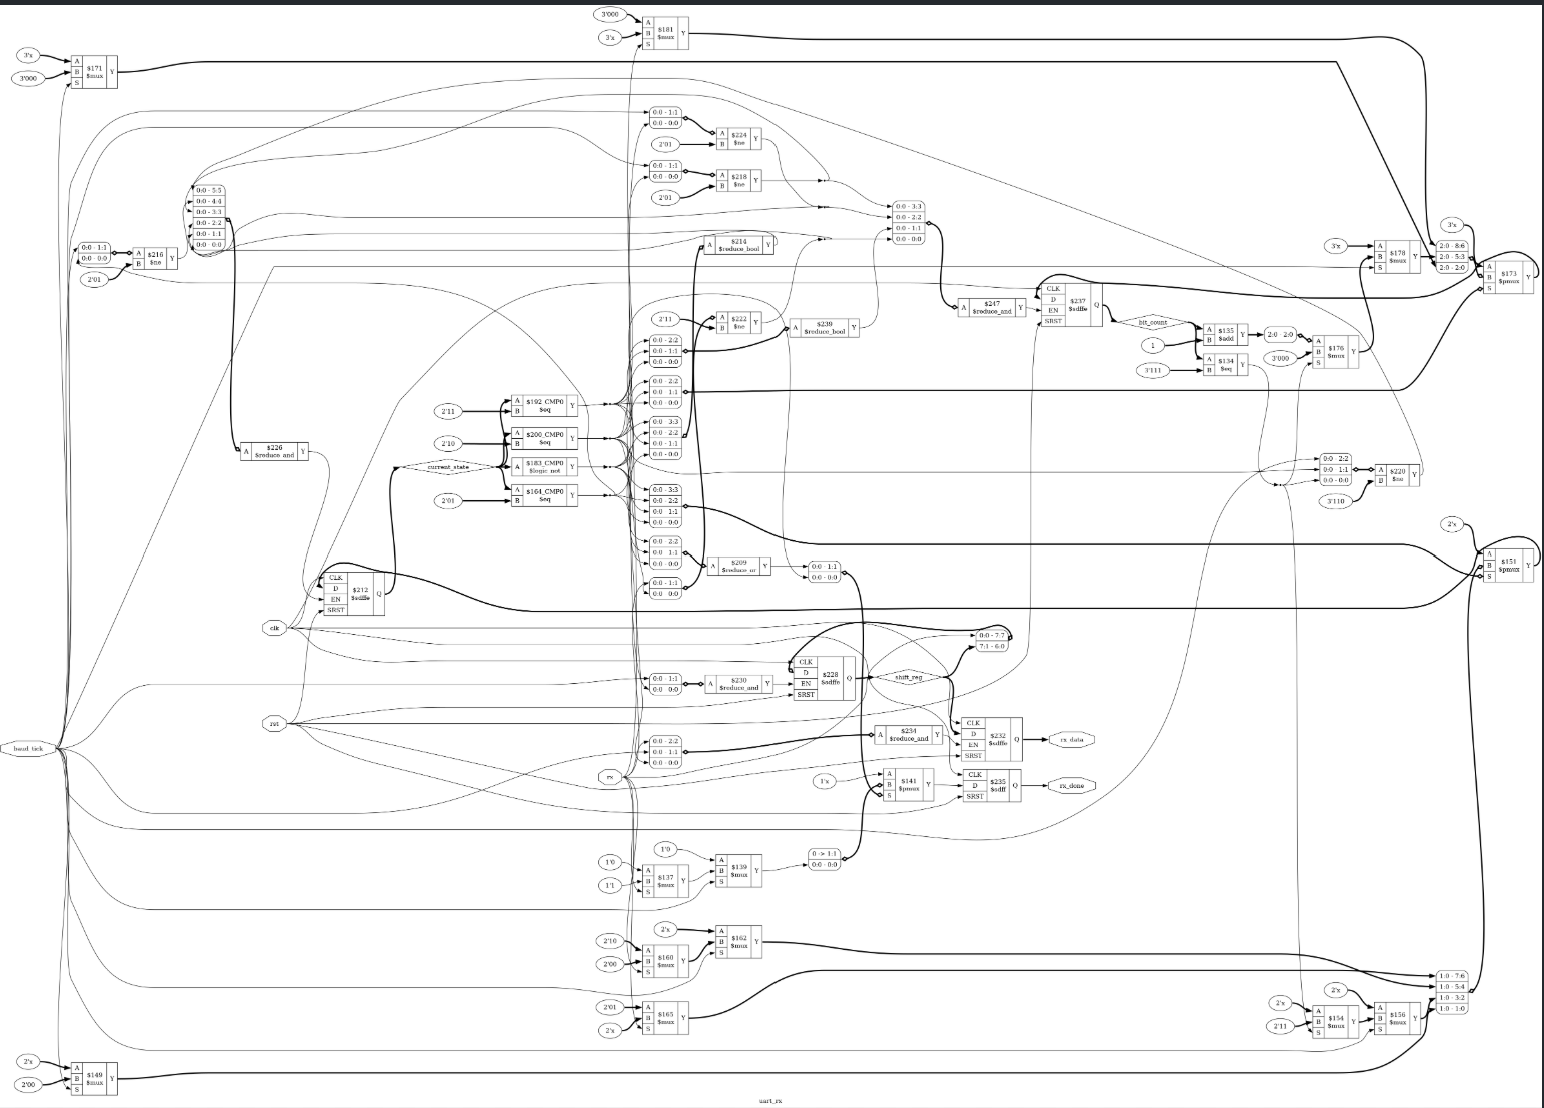
\includegraphics[width=\textwidth]{images/uart_rx_rtl.png}
\caption{RTL schematic of the UART receiver generated using Yosys.}
\label{fig:rx_rtl}
\end{figure}

%%%%%%%%%%%%%%%%%%%%%%%%%%%%%%%%%%%%%%%%%%%%%%%%%%%%%%%%%%%%

\section{UART Top Module}

The UART top module integrates the baud generator, transmitter and receiver into a complete UART IP core. The baud tick generated by the baud generator is shared by both transmitter and receiver to ensure synchronized operation.


\begin{figure}[!htbp]
\centering
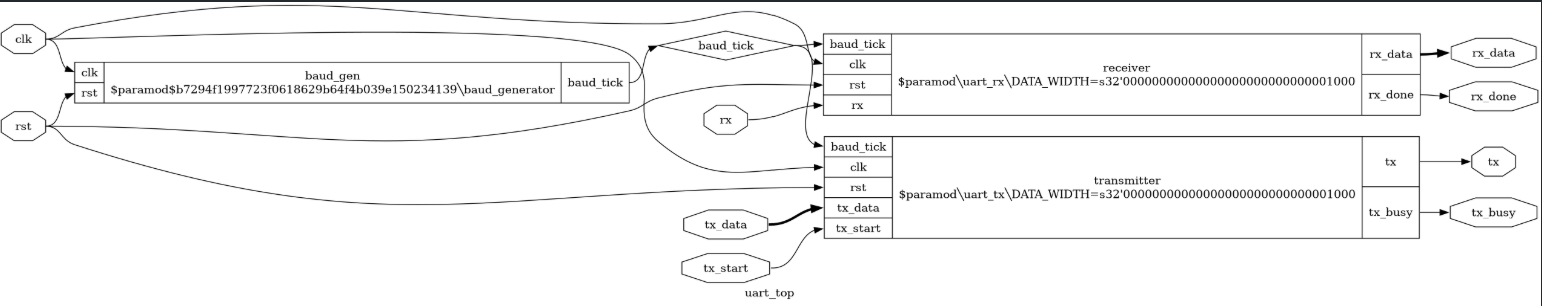
\includegraphics[width=\textwidth]{images/uart_top.png}
\caption{RTL hierarchy of the complete UART top module generated using Yosys.}
\label{fig:top_rtl}
\end{figure}

%%%%%%%%%%%%%%%%%%%%%%%%%%%%%%%%%%%%%%%%%%%%%%%%%%%%%%%%%%%%

\section{Functional Verification}

Each RTL module was verified independently using dedicated Verilog testbenches. After successful individual verification, the complete UART IP core was simulated to validate end-to-end serial communication.

The functional verification confirmed:

\begin{itemize}
\item Correct baud tick generation.
\item Proper UART frame transmission.
\item Accurate serial-to-parallel data reception.
\item Successful integration of transmitter, receiver and baud generator.
\end{itemize}

The simulation waveforms are presented in Chapter~\ref{chap:results}, where the functional behavior of each module is analyzed in detail.
\chapter{RTL-to-GDSII Design Flow Using OpenLane2}
\label{chap:rtl_to_gdsii}

This chapter describes the complete ASIC implementation flow used to transform the verified RTL design into a manufacturable GDSII layout. The implementation was performed using the open-source OpenLane2 flow, which integrates industry-standard tools for synthesis, physical design, routing, timing optimization, and physical verification.

The UART IP core was implemented using the SkyWater SKY130 open-source Process Design Kit (PDK). The design flow begins with synthesizable Verilog RTL and automatically progresses through logic synthesis, floorplanning, placement, clock tree synthesis, routing, and physical verification before generating the final GDSII layout.

%%%%%%%%%%%%%%%%%%%%%%%%%%%%%%%%%%%%%%%%%%%%%%%%%%%%%%%%%%%%%%%%%%%%%%%

\section{OpenLane2 Design Flow}

OpenLane2 provides an automated RTL-to-GDSII implementation flow by integrating multiple open-source EDA tools into a unified framework. The complete design flow used in this project is illustrated in Figure~\ref{fig:openlane_flow}.

\begin{figure}[!htbp]
\centering
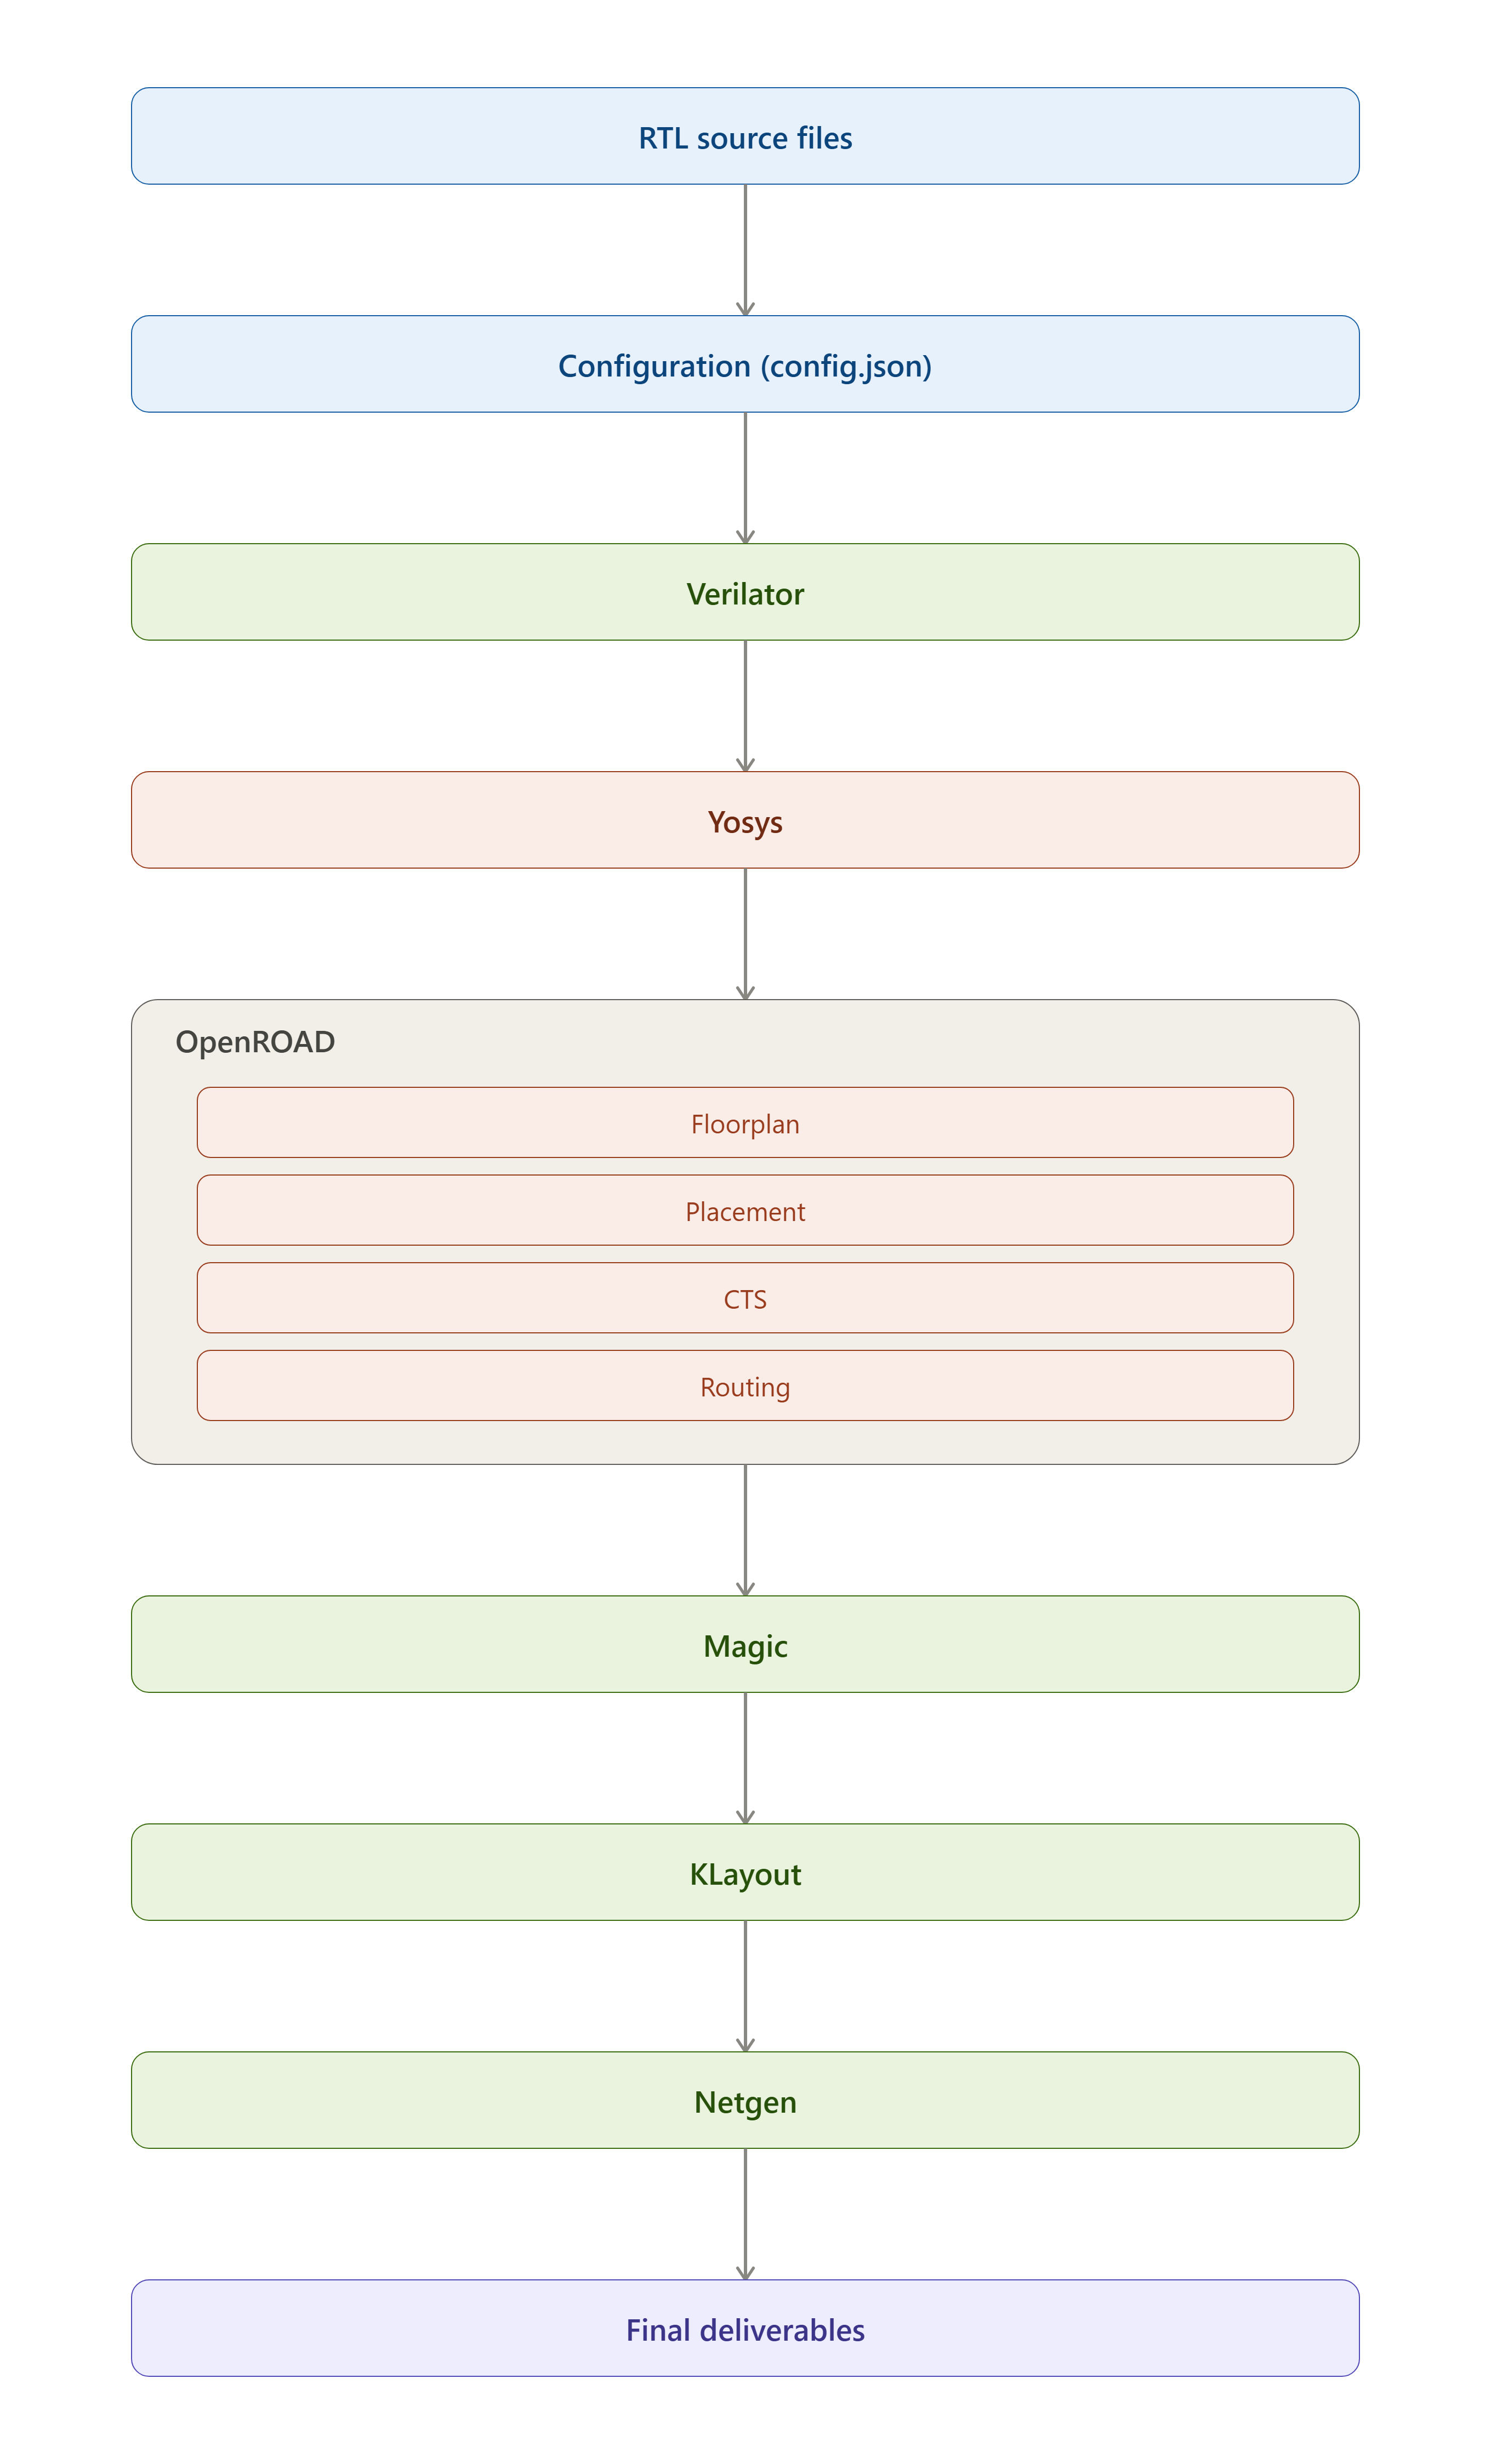
\includegraphics[width=0.85\textwidth]{images/openlane2_internal_workflow.png}
\caption{Complete RTL-to-GDSII implementation flow using OpenLane2.}
\label{fig:openlane_flow}
\end{figure}

The major stages of the implementation flow are summarized below.

\begin{table}[!htbp]
\centering
\caption{Major stages of the OpenLane2 ASIC design flow}
\label{tab:openlane_stages}
\begin{tabular}{ll}
\toprule
Stage & Description\\
\midrule
RTL Design & Verilog HDL implementation\\
RTL Linting & Design rule and syntax checking\\
Logic Synthesis & RTL converted into gate-level netlist\\
Floorplanning & Core and I/O planning\\
Placement & Standard cell placement\\
Clock Tree Synthesis & Clock distribution network generation\\
Routing & Signal interconnection\\
Physical Verification & DRC and LVS verification\\
GDSII Generation & Final layout generation\\
\bottomrule
\end{tabular}
\end{table}

%%%%%%%%%%%%%%%%%%%%%%%%%%%%%%%%%%%%%%%%%%%%%%%%%%%%%%%%%%%%%%%%%%%%%%%

\section{Project Directory Structure}

The UART project was organized into separate directories for RTL source files, testbenches, configuration files, simulation outputs, reports, and implementation results.
\begin{verbatim}
uart_asic_ip/
|
|-- rtl/
|   |-- uart_top.v
|   |-- uart_tx.v
|   |-- uart_rx.v
|   `-- baud_generator.v
|
|-- tb/
|
|-- waveforms/
|
|-- sim/
|
|-- config.json
|
|-- runs/
|
|-- reports/
|
|-- logs/
|
`-- results/
\end{verbatim}

This directory organization simplifies project management and separates design sources from generated implementation files.

%%%%%%%%%%%%%%%%%%%%%%%%%%%%%%%%%%%%%%%%%%%%%%%%%%%%%%%%%%%%%%%%%%%%%%%

\section{Design Configuration}

OpenLane2 uses a \texttt{config.json} file to define the design-specific implementation parameters. This configuration specifies the top module, RTL source files, target PDK, clock information, and implementation constraints.

The primary configuration parameters used in this project are summarized in Table~\ref{tab:config}.

\begin{table}[!htbp]
\centering
\caption{Important OpenLane2 configuration parameters}
\label{tab:config}
\begin{tabular}{ll}
\toprule
Parameter & Purpose\\
\midrule
DESIGN\_NAME & Top module name\\
VERILOG\_FILES & RTL source files\\
CLOCK\_PORT & Primary clock input\\
CLOCK\_PERIOD & Target clock period\\
PDK & SkyWater SKY130 PDK\\
STD\_CELL\_LIBRARY & SKY130 standard cells\\
\bottomrule
\end{tabular}
\end{table}

%%%%%%%%%%%%%%%%%%%%%%%%%%%%%%%%%%%%%%%%%%%%%%%%%%%%%%%%%%%%%%%%%%%%%%%

\section{RTL Linting Using Verilator}

Before synthesis, the RTL design was analyzed using Verilator to detect syntax errors, unsupported constructs, signal mismatches, and coding issues.

RTL linting improves design quality by identifying potential implementation problems before the synthesis stage. Successful completion of RTL linting ensures that the Verilog source files are suitable for logic synthesis.

%%%%%%%%%%%%%%%%%%%%%%%%%%%%%%%%%%%%%%%%%%%%%%%%%%%%%%%%%%%%%%%%%%%%%%%

\section{Logic Synthesis Using Yosys}

Logic synthesis converts the behavioral Verilog description into a technology-mapped gate-level netlist using the SkyWater SKY130 standard cell library.

The synthesis process includes RTL parsing, hierarchy checking, logic optimization, technology mapping, and netlist generation.

Figure~\ref{fig:yosys_flow} illustrates the major synthesis stages.

\begin{figure}[!htbp]
\centering
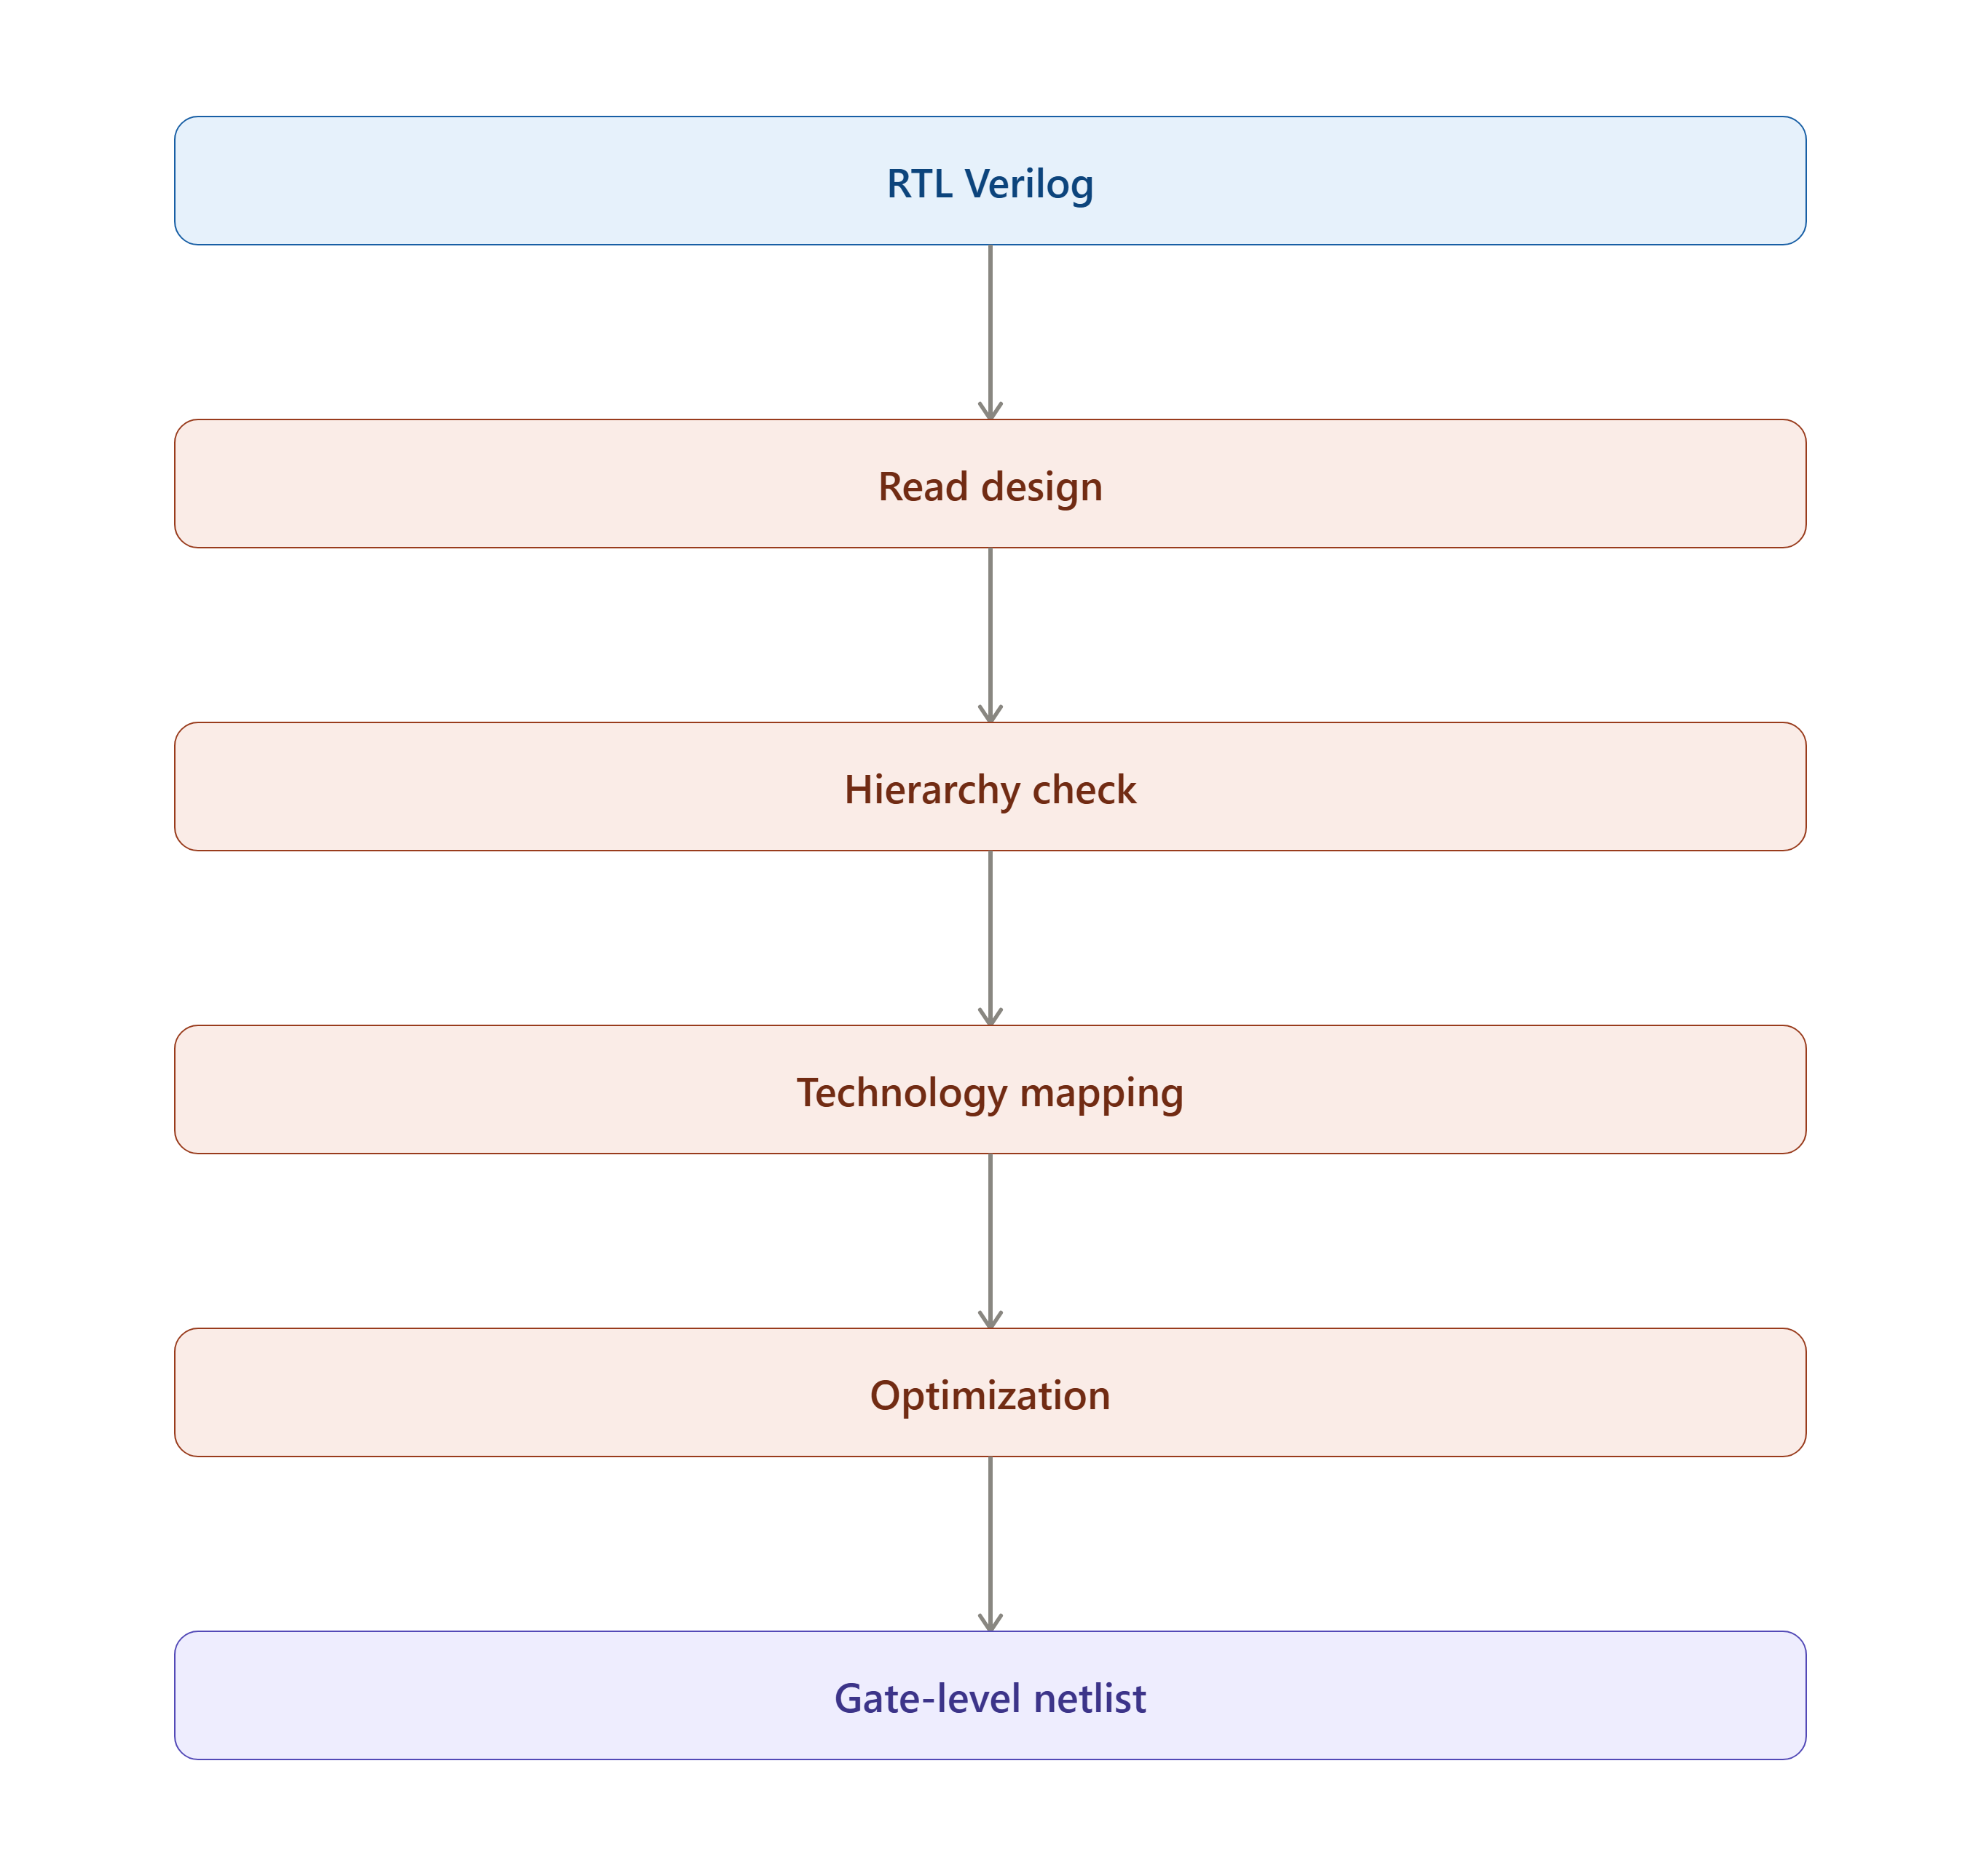
\includegraphics[width=0.78\textwidth]{images/synthesis_flow.png}
\caption{Logic synthesis flow performed using Yosys.}
\label{fig:yosys_flow}
\end{figure}

The synthesized gate-level netlist generated during this stage serves as the input for the subsequent physical design stages.

%%%%%%%%%%%%%%%%%%%%%%%%%%%%%%%%%%%%%%%%%%%%%%%%%%%%%%%%%%%%%%%%%%%%%%%

\section{Complete OpenLane2 Implementation Pipeline}

The overall implementation pipeline combines all open-source tools into a single automated ASIC design flow. Each tool performs a dedicated task and passes its output to the next stage until the final GDSII layout is produced.


Table~\ref{tab:eda_tools} summarizes the primary EDA tools used throughout the implementation flow.

\begin{table}[!htbp]
\centering
\caption{Open-source EDA tools used in this project}
\label{tab:eda_tools}
\begin{tabular}{ll}
\toprule
Tool & Function\\
\midrule
Verilator & RTL linting and design checking\\
Yosys & Logic synthesis\\
OpenROAD & Physical implementation\\
Magic & Layout generation and DRC\\
KLayout & Layout visualization and DRC\\
Netgen & Layout versus schematic (LVS) verification\\
\bottomrule
\end{tabular}
\end{table}

The outputs generated during each stage of the implementation flow are summarized in Table~\ref{tab:outputs}.

\begin{table}[!htbp]
\centering
\caption{Generated outputs during RTL-to-GDSII implementation}
\label{tab:outputs}
\begin{tabular}{ll}
\toprule
Stage & Output\\
\midrule
RTL Design & Verilog source files\\
Logic Synthesis & Gate-level netlist\\
Floorplanning & Floorplan DEF\\
Placement & Placed DEF\\
CTS & Clock tree\\
Routing & Routed DEF\\
Physical Verification & DRC and LVS reports\\
Final Output & GDSII layout\\
\bottomrule
\end{tabular}
\end{table}

The detailed implementation of floorplanning, placement, clock tree synthesis, routing, and physical verification is presented in the following chapters.
\chapter{Physical Design Implementation}
\label{chap:physical_design}

After logic synthesis, the gate-level netlist was imported into the OpenROAD engine through the OpenLane2 flow for physical implementation. This stage transforms the logical design into a manufacturable layout by determining standard cell locations, constructing the clock network, and routing signal interconnections. Using the SkyWater SKY130 PDK, OpenLane2 automatically performed floorplanning, placement, clock tree synthesis (CTS), global routing, and detailed routing.

\begin{figure}[!htbp]
    \centering
    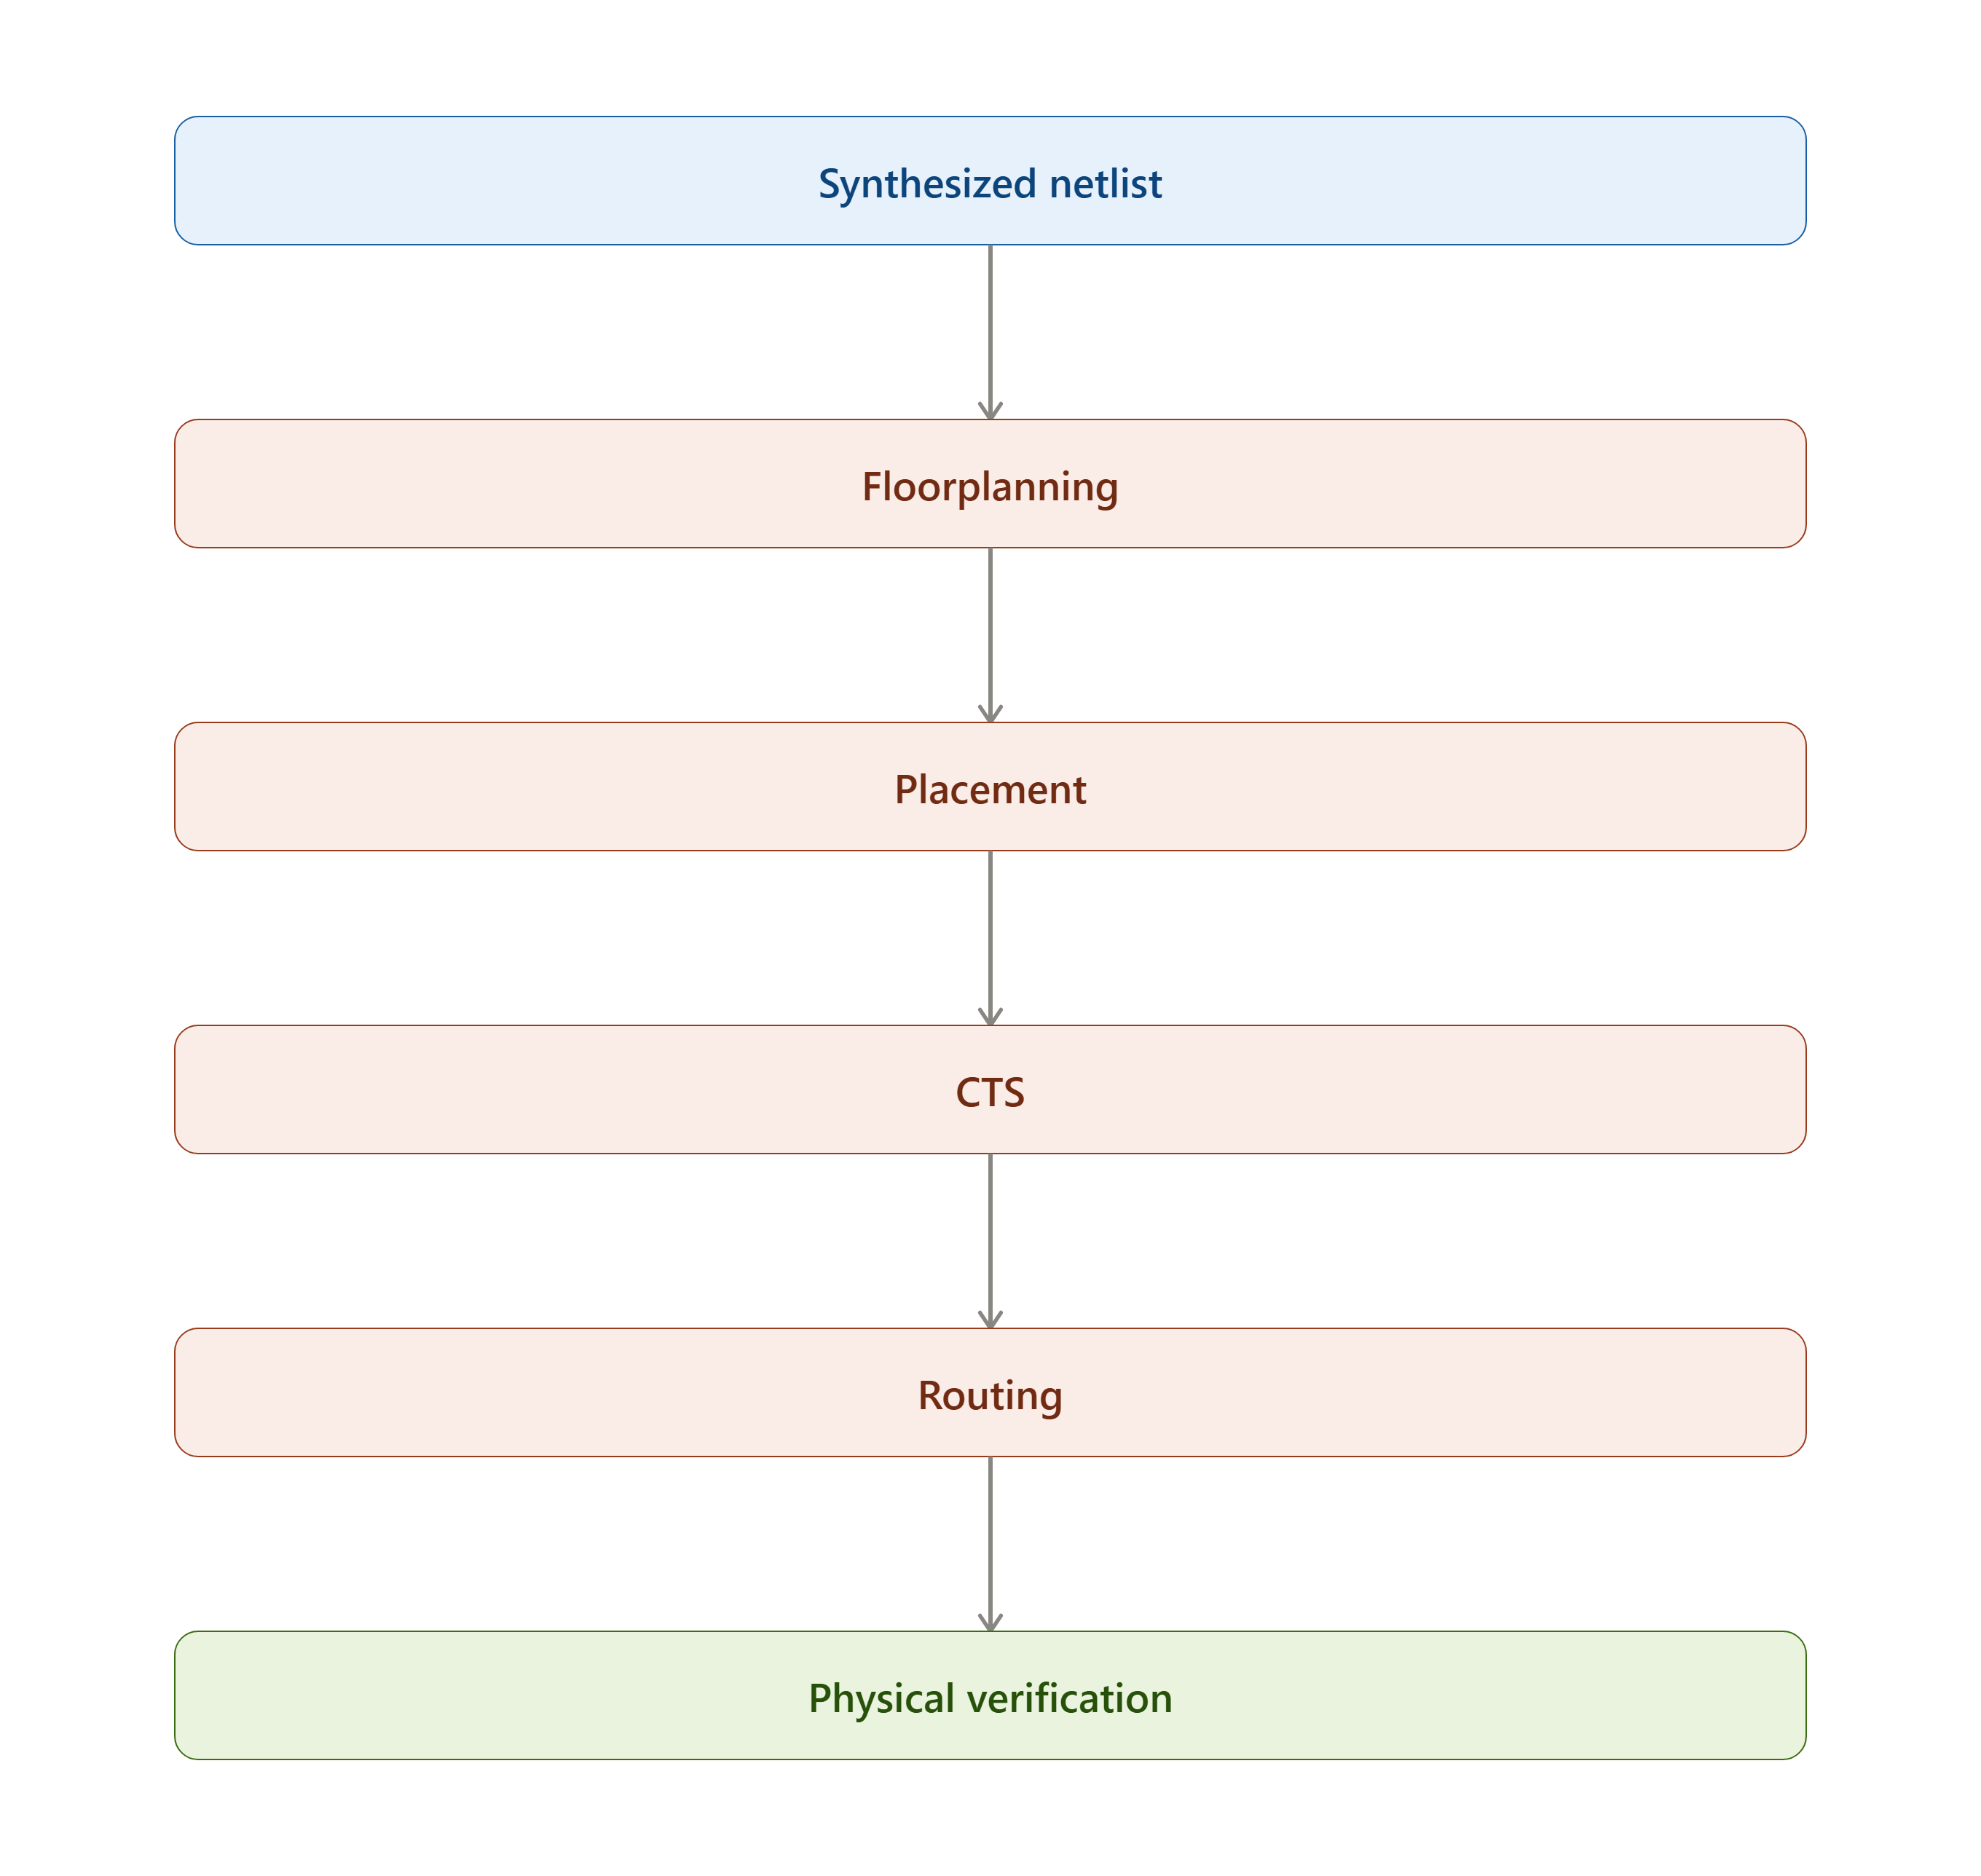
\includegraphics[width=0.88\textwidth]{images/physical_design_flow.png}
    \caption{Physical design implementation flow using OpenROAD.}
    \label{fig:physical_design_flow}
\end{figure}


%%%%%%%%%%%%%%%%%%%%%%%%%%%%%%%%%%%%%%%%%%%%%%%%%%%%%%%%%%%%%%%

\section{Floorplanning}

Floorplanning is the first stage of physical implementation where the die area, core area, placement rows, utilization, and I/O pin locations are established. A well-planned floorplan provides sufficient routing resources and minimizes congestion during later stages of implementation.

Figure~\ref{fig:floorplan} shows the generated floorplan of the UART IP core obtained from OpenROAD.

\begin{figure}[!htbp]
    \centering
    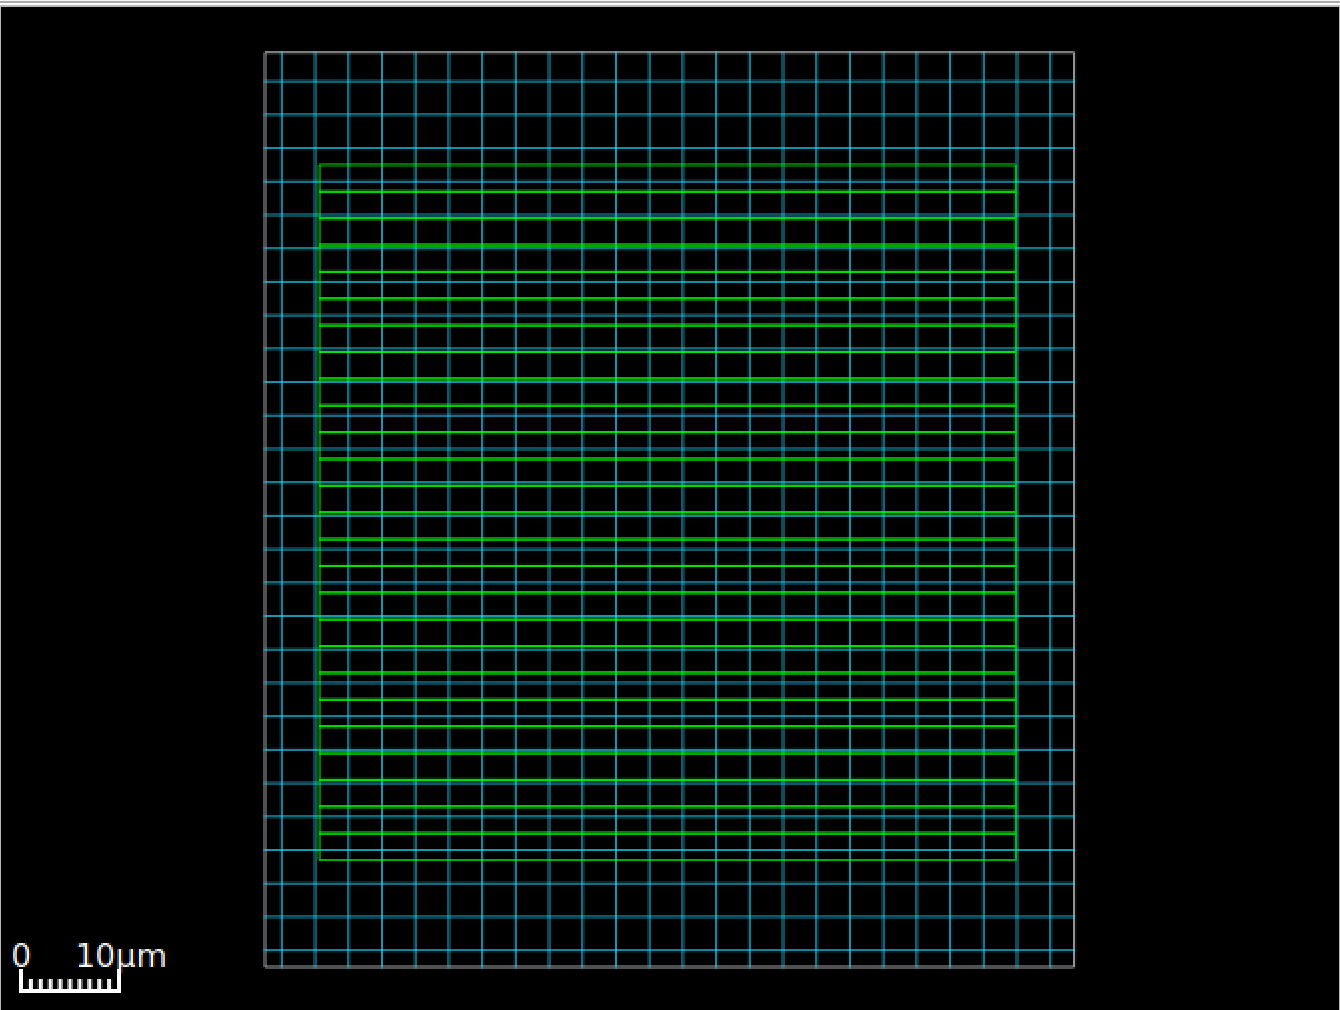
\includegraphics[width=0.93\textwidth]{images/Standard_Cell_Rows_Generated_During_Floorplanning.png}
    \caption{Generated floorplan of the UART ASIC design.}
    \label{fig:floorplan}
\end{figure}

The floorplanning report generated during implementation is summarized in Table~\ref{tab:floorplan_metrics}.

\begin{table}[!htbp]
\centering
\caption{Floorplanning metrics}
\label{tab:floorplan_metrics}
\begin{tabular}{lc}
\toprule
Parameter & Value\\
\midrule
Die Area & 7658.18 $\mu m^2$\\
Core Area & 5009.80 $\mu m^2$\\
Standard Cell Area & 3210.58 $\mu m^2$\\
Instance Count & 375\\
Core Utilization & 64.09\%\\
I/O Pins & 25\\
\bottomrule
\end{tabular}
\end{table}

The generated floorplan achieved a core utilization of approximately 64\%, providing sufficient whitespace for placement optimization and routing while maintaining an efficient silicon area.

%%%%%%%%%%%%%%%%%%%%%%%%%%%%%%%%%%%%%%%%%%%%%%%%%%%%%%%%%%%%%%%

\section{Global and Detailed Placement}

After floorplanning, OpenROAD performs global placement to determine approximate locations of all standard cells while minimizing wirelength and improving timing. This is followed by detailed placement, where every standard cell is aligned to legal placement rows and overlap violations are removed.

Figure~\ref{fig:placement} shows the placed standard-cell layout generated during the placement stage.

\begin{figure}[!htbp]
    \centering
    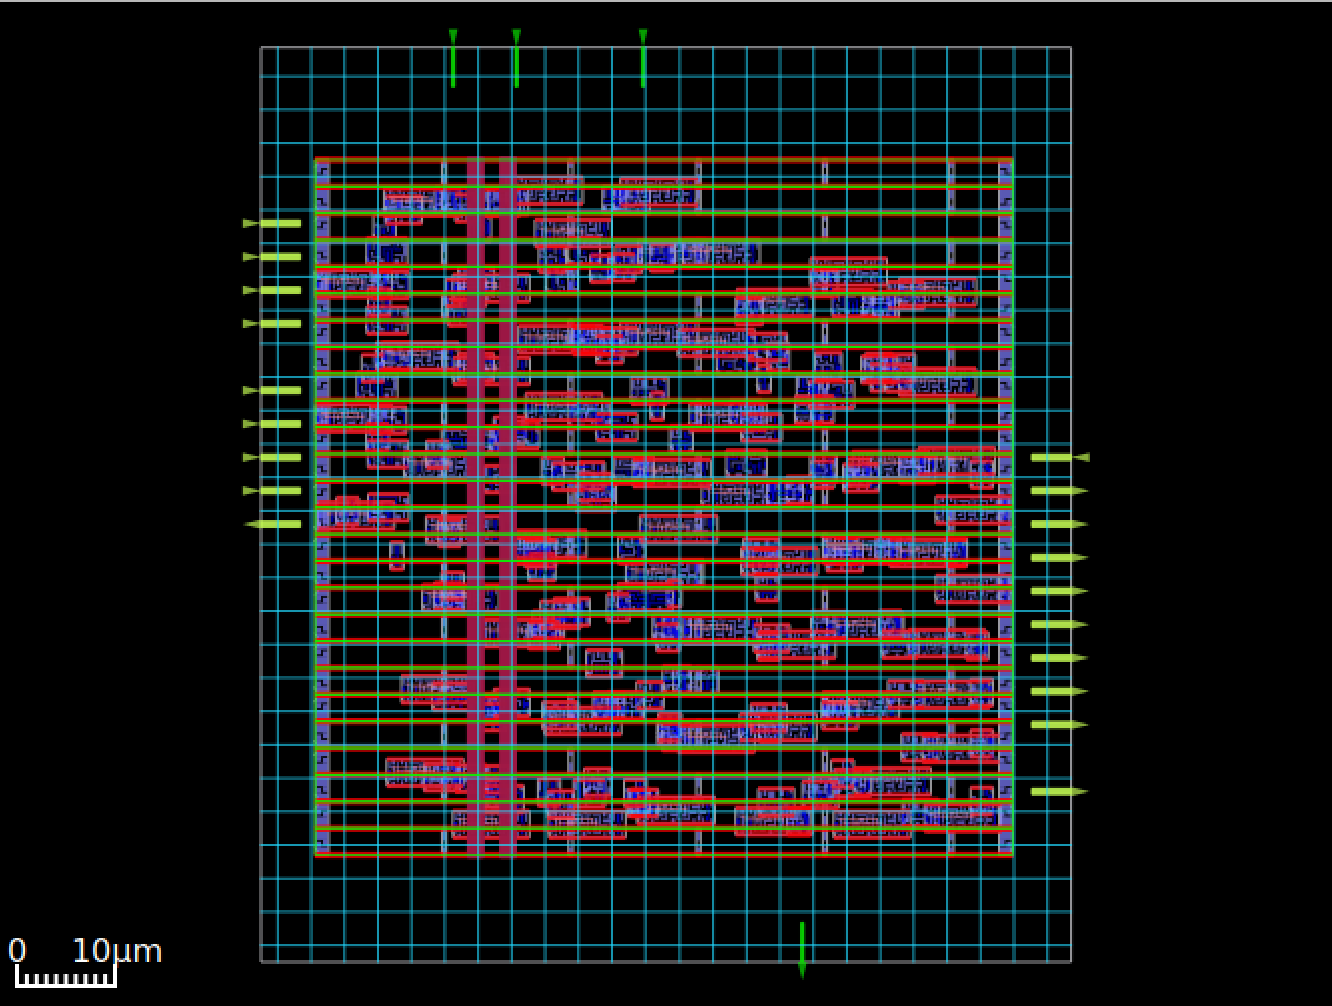
\includegraphics[width=0.93\textwidth]{images/Standard_Cell_Placement.png}
    \caption{Standard-cell placement generated by OpenROAD.}
    \label{fig:placement}
\end{figure}

The placement statistics obtained from the OpenLane2 implementation are summarized in Table~\ref{tab:placement_metrics}.

\begin{table}[H]
\centering
\caption{Placement metrics}
\label{tab:placement_metrics}
\begin{tabular}{lc}
\toprule
Parameter & Value\\
\midrule
Total Displacement & 0.0 $\mu$m\\
Average Displacement & 0.0 $\mu$m\\
Maximum Displacement & 0.0 $\mu$m\\
HPWL Before Optimization & 3351.5 $\mu$m\\
HPWL After Optimization & 3207.2 $\mu$m\\
HPWL Improvement & 4.3\%\\
Standard Cell Utilization & 51.65\%\\
\bottomrule
\end{tabular}
\end{table}

OpenROAD also inserted additional cells required for placement legalization and timing optimization. The resulting cell distribution is shown in Table~\ref{tab:placement_cells}.

\begin{table}[H]
\centering
\caption{Cell distribution after detailed placement}
\label{tab:placement_cells}
\begin{tabular}{lc}
\toprule
Cell Type & Count\\
\midrule
Sequential Cells & 55\\
Combinational Cells & 156\\
Timing Repair Buffers & 31\\
Tap Cells & 70\\
Fill Cells & 52\\
Inverters & 8\\
Total Cells & 372\\
\bottomrule
\end{tabular}
\end{table}

The detailed placement stage completed without overlap violations. The reported zero displacement indicates that all standard cells were successfully legalized while preserving the optimized placement generated during global placement. Furthermore, the reduction in Half-Perimeter Wire Length (HPWL) after optimization demonstrates improved routing efficiency and timing quality.


%%%%%%%%%%%%%%%%%%%%%%%%%%%%%%%%%%%%%%%%%%%%%%%%%%%%%%%%%%%%%%%

\section{Clock Tree Synthesis}

Clock Tree Synthesis (CTS) is performed after placement to distribute the clock signal uniformly to all sequential elements while minimizing clock skew, insertion delay, and timing violations. During this stage, OpenROAD inserts clock buffers and inverters to construct an optimized clock distribution network.

Figure~\ref{fig:cts} shows the CTS stage.

\begin{figure}[!htbp]
    \centering
    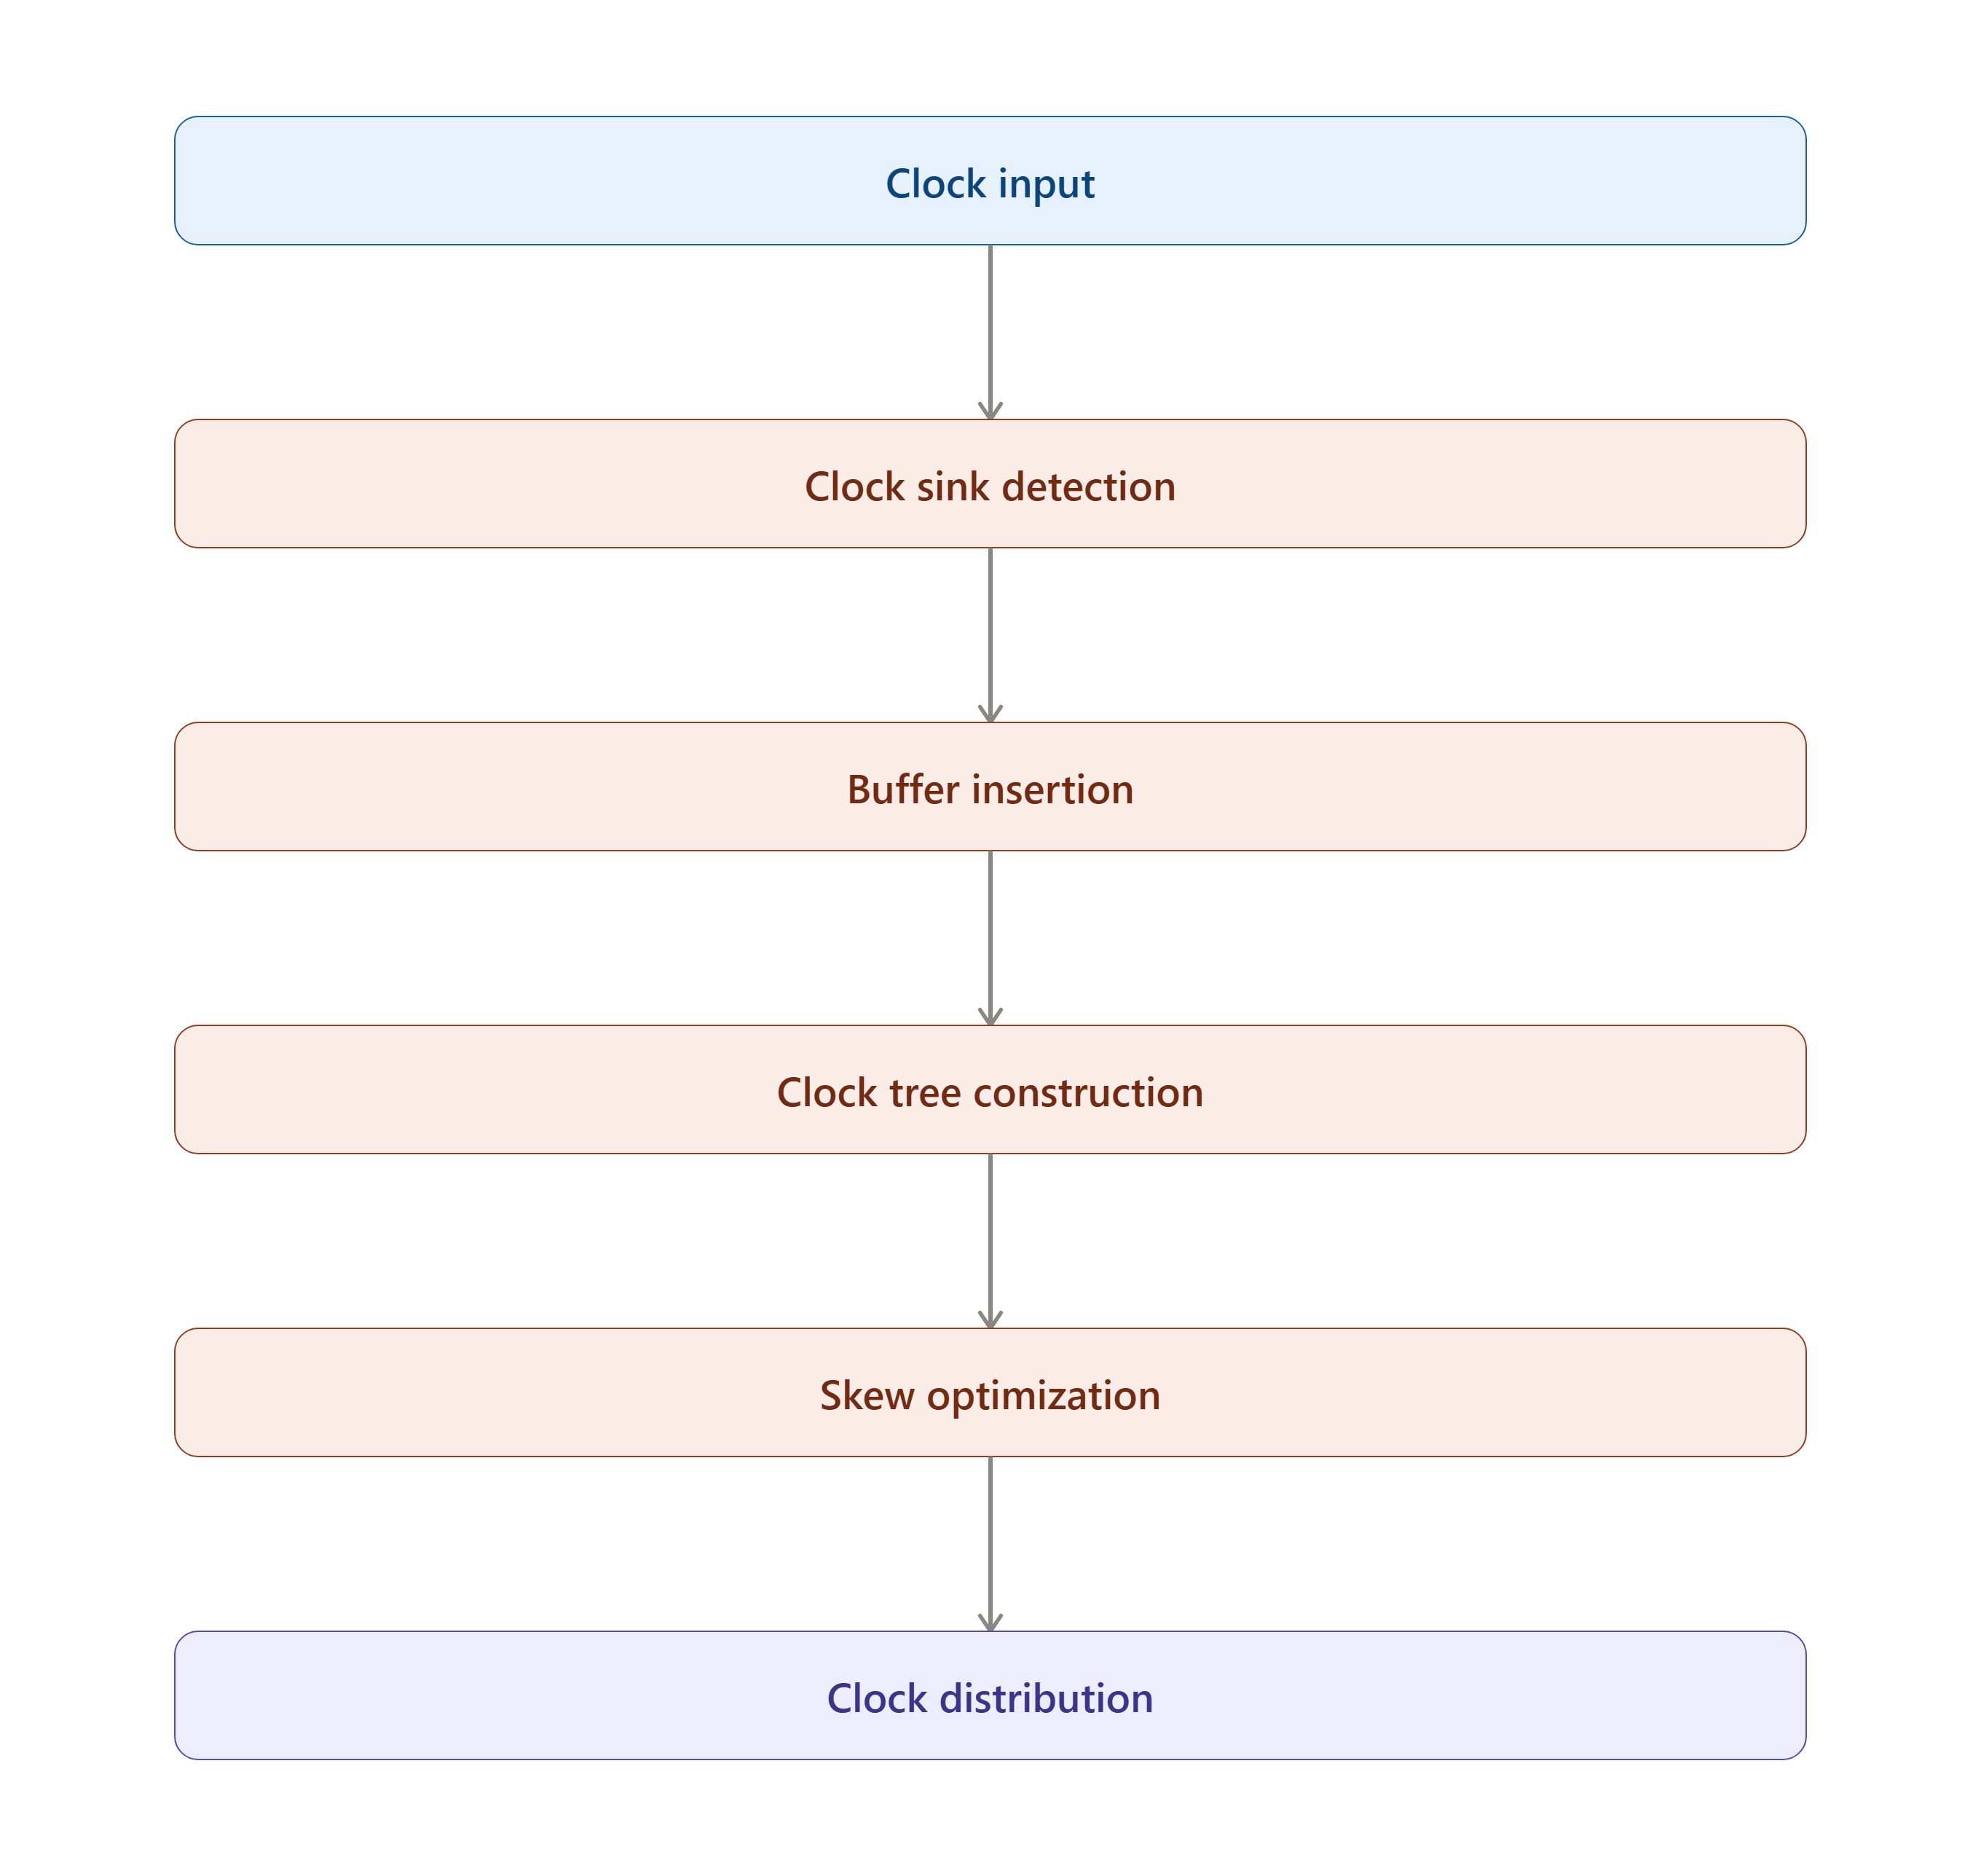
\includegraphics[width=0.93\textwidth]{images/clock_tree_synthesis.png}
    \caption{Clock Tree Synthesis (CTS) stages.}
    \label{fig:cts}
\end{figure}

The CTS report generated during implementation is summarized in Table~\ref{tab:cts_metrics}.

\begin{table}[H]
\centering
\caption{Clock Tree Synthesis statistics}
\label{tab:cts_metrics}
\begin{tabular}{lc}
\toprule
Parameter & Value\\
\midrule
Clock Nets & 6\\
Clock Buffers Inserted & 5\\
Clock Inverters Inserted & 3\\
Timing Repair Buffers & 78\\
Sequential Cells & 55\\
Total Cell Instances & 427\\
Total Cell Area & 3405.77 $\mu m^2$\\
Core Utilization & 64.09\%\\
\bottomrule
\end{tabular}
\end{table}

The CTS stage successfully generated the clock distribution network without introducing clock-related violations. The insertion of dedicated clock buffers and inverters balanced the clock paths while maintaining acceptable utilization. Additional timing repair buffers were inserted automatically by OpenROAD to improve timing performance before routing.


%%%%%%%%%%%%%%%%%%%%%%%%%%%%%%%%%%%%%%%%%%%%%%%%%%%%%%%%%%%%%%%

\section{Global and Detailed Routing}

Following Clock Tree Synthesis (CTS), OpenROAD performs routing to establish all electrical connections between the placed standard cells. The routing process consists of two stages: global routing, which determines approximate routing paths, and detailed routing, which generates the final metal interconnections while satisfying the SKY130 design rules.

Figure~\ref{fig:routing} shows the routed layout generated after the completion of detailed routing.

\begin{figure}[!htbp]
    \centering
    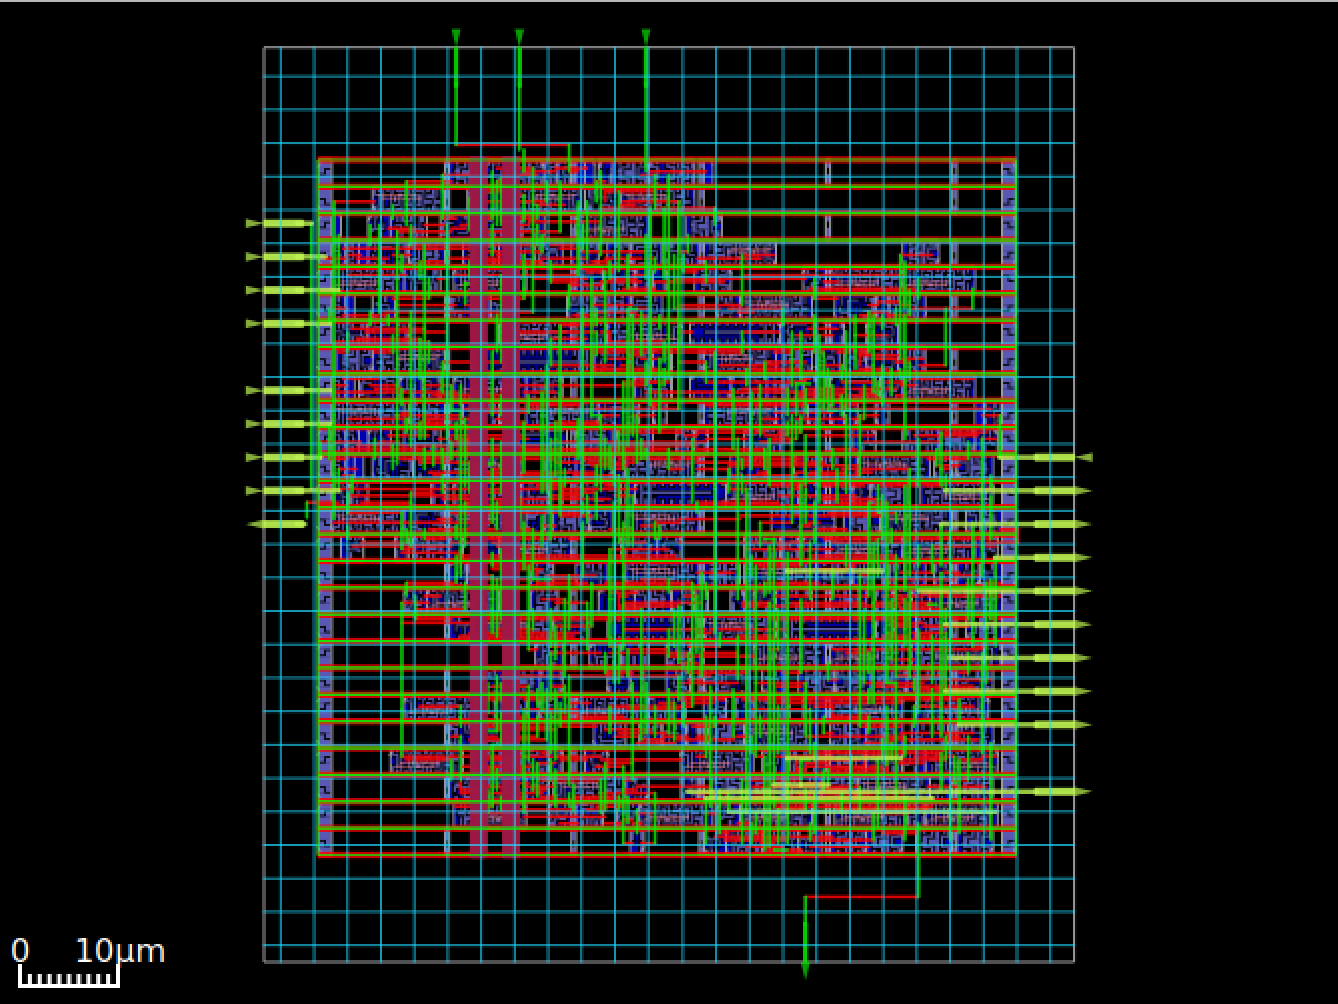
\includegraphics[width=0.93\textwidth]{images/Final_Detailed Routed_Layout_of_the_UART_ASIC.png}
    \caption{Final routed layout generated by OpenROAD.}
    \label{fig:routing}
\end{figure}

The routing stage completed successfully without any congestion or overflow. Table~\ref{tab:routing_metrics} summarizes the routing statistics obtained from the OpenLane2 implementation.

\begin{table}[!htbp]
\centering
\caption{Global and detailed routing statistics}
\label{tab:routing_metrics}
\begin{tabular}{lc}
\toprule
Parameter & Value\\
\midrule
Routed Nets & 314\\
Total Wirelength & 8404 $\mu$m\\
Total Vias & 1804\\
Routing Resource Usage & 14.71\%\\
Routing Overflow & 0\\
Antenna Violating Nets & 0\\
Antenna Violating Pins & 0\\
\bottomrule
\end{tabular}
\end{table}

The routing resource utilization for each metal layer is summarized in Table~\ref{tab:layer_usage}.

\begin{table}[!htbp]
\centering
\caption{Routing resource utilization by metal layer}
\label{tab:layer_usage}
\begin{tabular}{lccc}
\toprule
Layer & Resources & Demand & Usage\\
\midrule
Metal1 & 1406 & 330 & 23.47\%\\
Metal2 & 1428 & 311 & 21.78\%\\
Metal3 & 940 & 17 & 1.81\%\\
Metal4 & 558 & 0 & 0.00\%\\
Metal5 & 140 & 0 & 0.00\%\\
\bottomrule
\end{tabular}
\end{table}

The routing results demonstrate efficient utilization of the available routing resources. The absence of routing overflow confirms that all signal nets were successfully connected without congestion. Furthermore, no antenna violations were reported, indicating that the routing satisfies the manufacturing requirements of the SKY130 process.

%%%%%%%%%%%%%%%%%%%%%%%%%%%%%%%%%%%%%%%%%%%%%%%%%%%%%%%%%%%%%%%

\section{Physical Design Summary}

Table~\ref{tab:physical_summary} summarizes the key results obtained throughout the physical design implementation.

\begin{table}[!htbp]
\centering
\caption{Summary of physical design implementation}
\label{tab:physical_summary}
\begin{tabular}{lc}
\toprule
Metric & Value\\
\midrule
Design Instances & 375\\
Core Area & 5009.80 $\mu m^2$\\
Die Area & 7658.18 $\mu m^2$\\
Core Utilization & 64.09\%\\
Clock Nets & 6\\
Clock Buffers & 5\\
Clock Inverters & 3\\
Timing Repair Buffers & 78\\
Routed Nets & 314\\
Wirelength & 8404 $\mu$m\\
Total Vias & 1804\\
Routing Overflow & 0\\
Antenna Violations & 0\\
\bottomrule
\end{tabular}
\end{table}

The physical implementation of the UART IP core was successfully completed using the OpenLane2 flow. All implementation stages, including floorplanning, placement, clock tree synthesis, and routing, were completed without critical issues. The generated routed layout serves as the input for the physical verification and signoff process presented in the next chapter.
\chapter{Physical Verification and Signoff}
\label{chap:physical_verification}

After the completion of physical implementation, the UART layout was subjected to a comprehensive verification process to ensure that the generated design satisfies timing, power integrity, layout correctness, and manufacturability requirements. The verification stages were performed using the integrated tools available in the OpenLane2 flow, including OpenRCX, OpenSTA, Magic, Netgen, and the manufacturability checker.

%%%%%%%%%%%%%%%%%%%%%%%%%%%%%%%%%%%%%%%%%%%%%%%%%%%%%%%%%%%%%%%

\section{Verification Flow}

The verification stages performed after routing are illustrated in Figure~\ref{fig:verification_flow}.

\begin{figure}[!htbp]
    \centering
    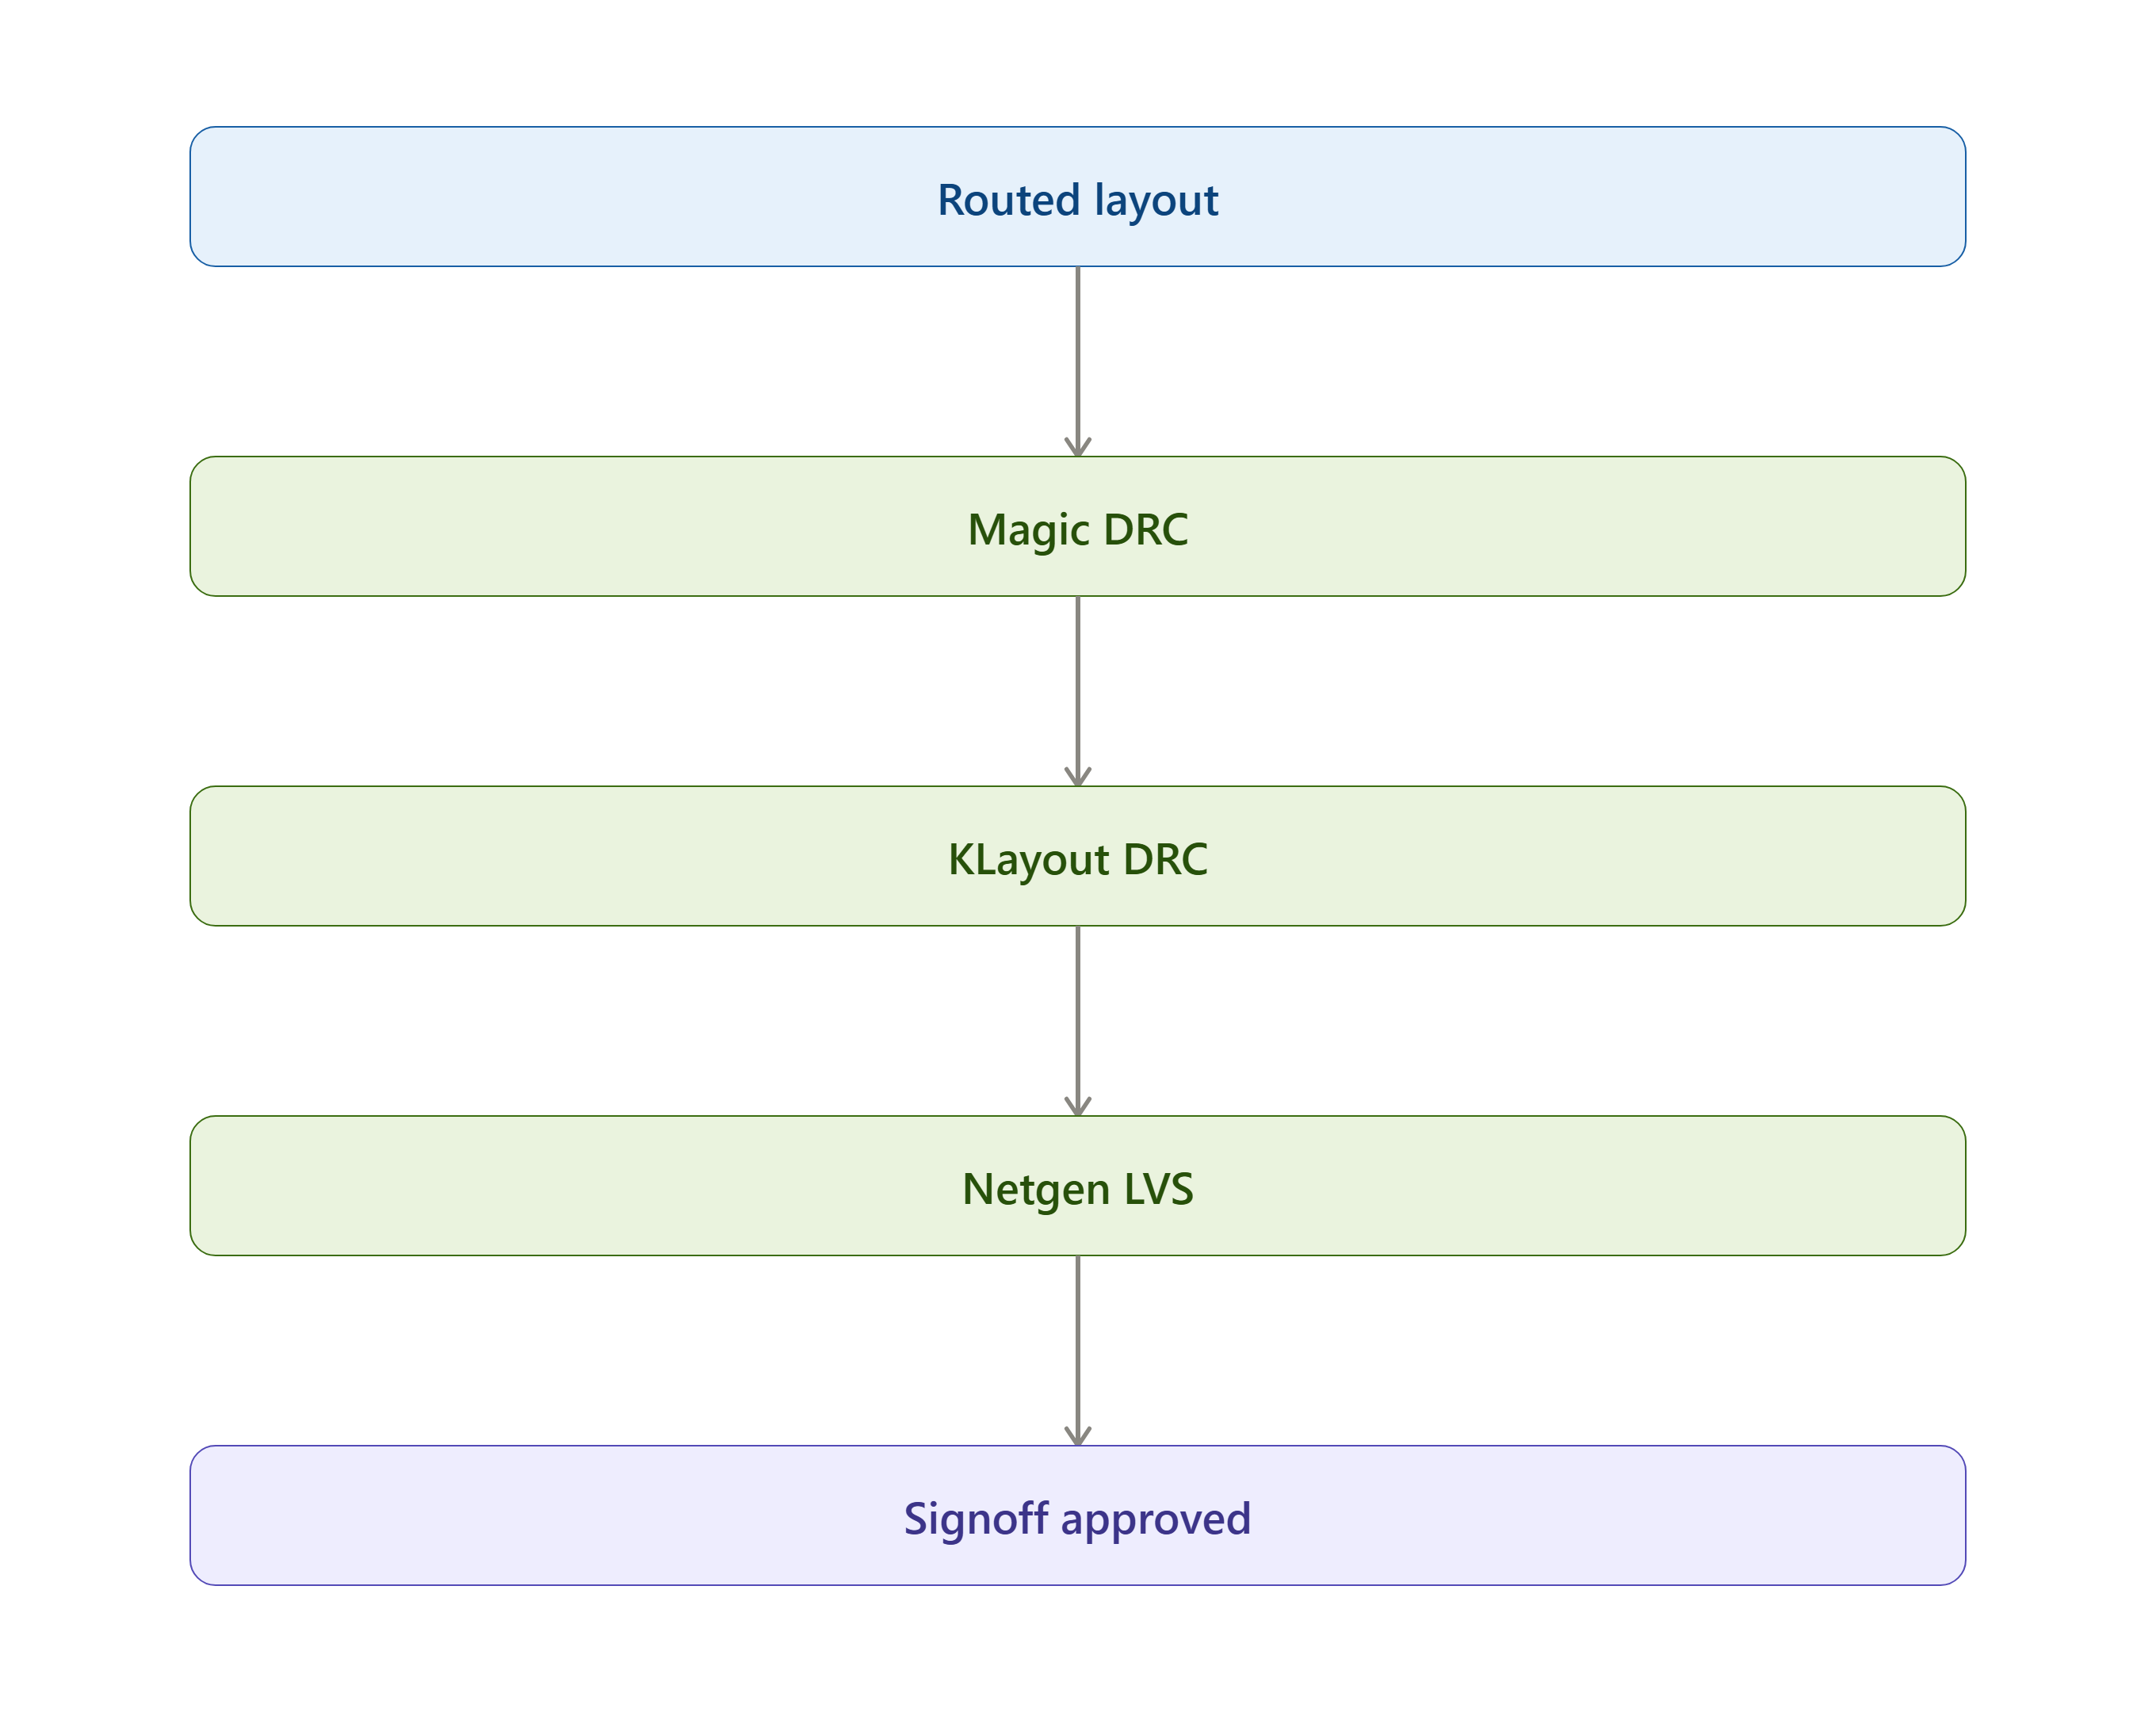
\includegraphics[width=0.86\textwidth]{images/physical_verification.png}
    \caption{Physical verification and signoff flow.}
    \label{fig:verification_flow}
\end{figure}

%%%%%%%%%%%%%%%%%%%%%%%%%%%%%%%%%%%%%%%%%%%%%%%%%%%%%%%%%%%%%%%

\section{RC Extraction}

After routing, parasitic resistance and capacitance associated with the interconnects were extracted using OpenRCX. The extracted parasitic information was stored in Standard Parasitic Exchange Format (SPEF) files and used for accurate post-layout timing analysis.

The RC extraction stage generated parasitic information for multiple process corners, as summarized in Table~\ref{tab:rcx_outputs}.

\begin{table}[!htbp]
\centering
\caption{Generated SPEF files}
\label{tab:rcx_outputs}
\begin{tabular}{ll}
\toprule
Operating Corner & Generated File\\
\midrule
Minimum & uart\_top.min.spef\\
Nominal & uart\_top.nom.spef\\
Maximum & uart\_top.max.spef\\
\bottomrule
\end{tabular}
\end{table}

The successful generation of all three SPEF files confirms that parasitic extraction was completed successfully without any extraction errors.

%%%%%%%%%%%%%%%%%%%%%%%%%%%%%%%%%%%%%%%%%%%%%%%%%%%%%%%%%%%%%%%

\section{Static Timing Analysis}

Static Timing Analysis (STA) was performed using the extracted parasitic information to verify timing performance under multiple operating corners.

The timing analysis evaluated setup and hold constraints across different process, voltage, and temperature (PVT) conditions. The analysis completed successfully without reporting critical timing violations, indicating successful timing closure after routing.

%%%%%%%%%%%%%%%%%%%%%%%%%%%%%%%%%%%%%%%%%%%%%%%%%%%%%%%%%%%%%%%

\section{IR Drop Analysis}

Power integrity analysis was performed to evaluate voltage drops across the power distribution network. The analysis confirmed that both the power (VPWR) and ground (VGND) networks maintain stable operating voltages throughout the design.

The measured voltage drops are summarized in Table~\ref{tab:irdrop_results}.

\begin{table}[!htbp]
\centering
\caption{IR-drop analysis results}
\label{tab:irdrop_results}
\begin{tabular}{lcc}
\toprule
Parameter & VPWR & VGND\\
\midrule
Worst Voltage & 1.79984 V & 0.000233 V\\
Average IR Drop & 0.0000416 V & 0.0000400 V\\
Worst IR Drop & 0.0001605 V & 0.0002330 V\\
Percentage Drop & 0.01\% & 0.01\%\\
\bottomrule
\end{tabular}
\end{table}

The observed voltage drop is extremely small, indicating a robust power distribution network suitable for reliable circuit operation.

%%%%%%%%%%%%%%%%%%%%%%%%%%%%%%%%%%%%%%%%%%%%%%%%%%%%%%%%%%%%%%%

\section{Design Rule Checking}

Magic was used to perform Design Rule Checking (DRC) on the routed layout. The generated layout was verified against the SKY130 manufacturing design rules.

The verification completed successfully with zero DRC violations.

\begin{table}[!htbp]
\centering
\caption{Magic DRC summary}
\label{tab:drc_summary}
\begin{tabular}{lc}
\toprule
Parameter & Result\\
\midrule
DRC Violations & 0\\
Verification Status & PASS\\
\bottomrule
\end{tabular}
\end{table}

%%%%%%%%%%%%%%%%%%%%%%%%%%%%%%%%%%%%%%%%%%%%%%%%%%%%%%%%%%%%%%%

\section{Layout Versus Schematic Verification}

Netgen was used to perform Layout Versus Schematic (LVS) verification. This step compares the extracted layout netlist against the synthesized gate-level netlist to ensure logical equivalence.


The LVS verification completed successfully, confirming that the physical layout matches the intended circuit implementation.

\begin{table}[!htbp]
\centering
\caption{LVS verification summary}
\label{tab:lvs_summary}
\begin{tabular}{lc}
\toprule
Parameter & Result\\
\midrule
Layout Matches Schematic & PASS\\
Verification Status & PASS\\
\bottomrule
\end{tabular}
\end{table}

%%%%%%%%%%%%%%%%%%%%%%%%%%%%%%%%%%%%%%%%%%%%%%%%%%%%%%%%%%%%%%%

\section{Final GDSII Layout}

The verified UART layout was exported in GDSII format after successful completion of all implementation and verification stages. Figure~\ref{fig:gds_layout} shows the final layout viewed in KLayout.

\begin{figure}[!htbp]
    \centering
    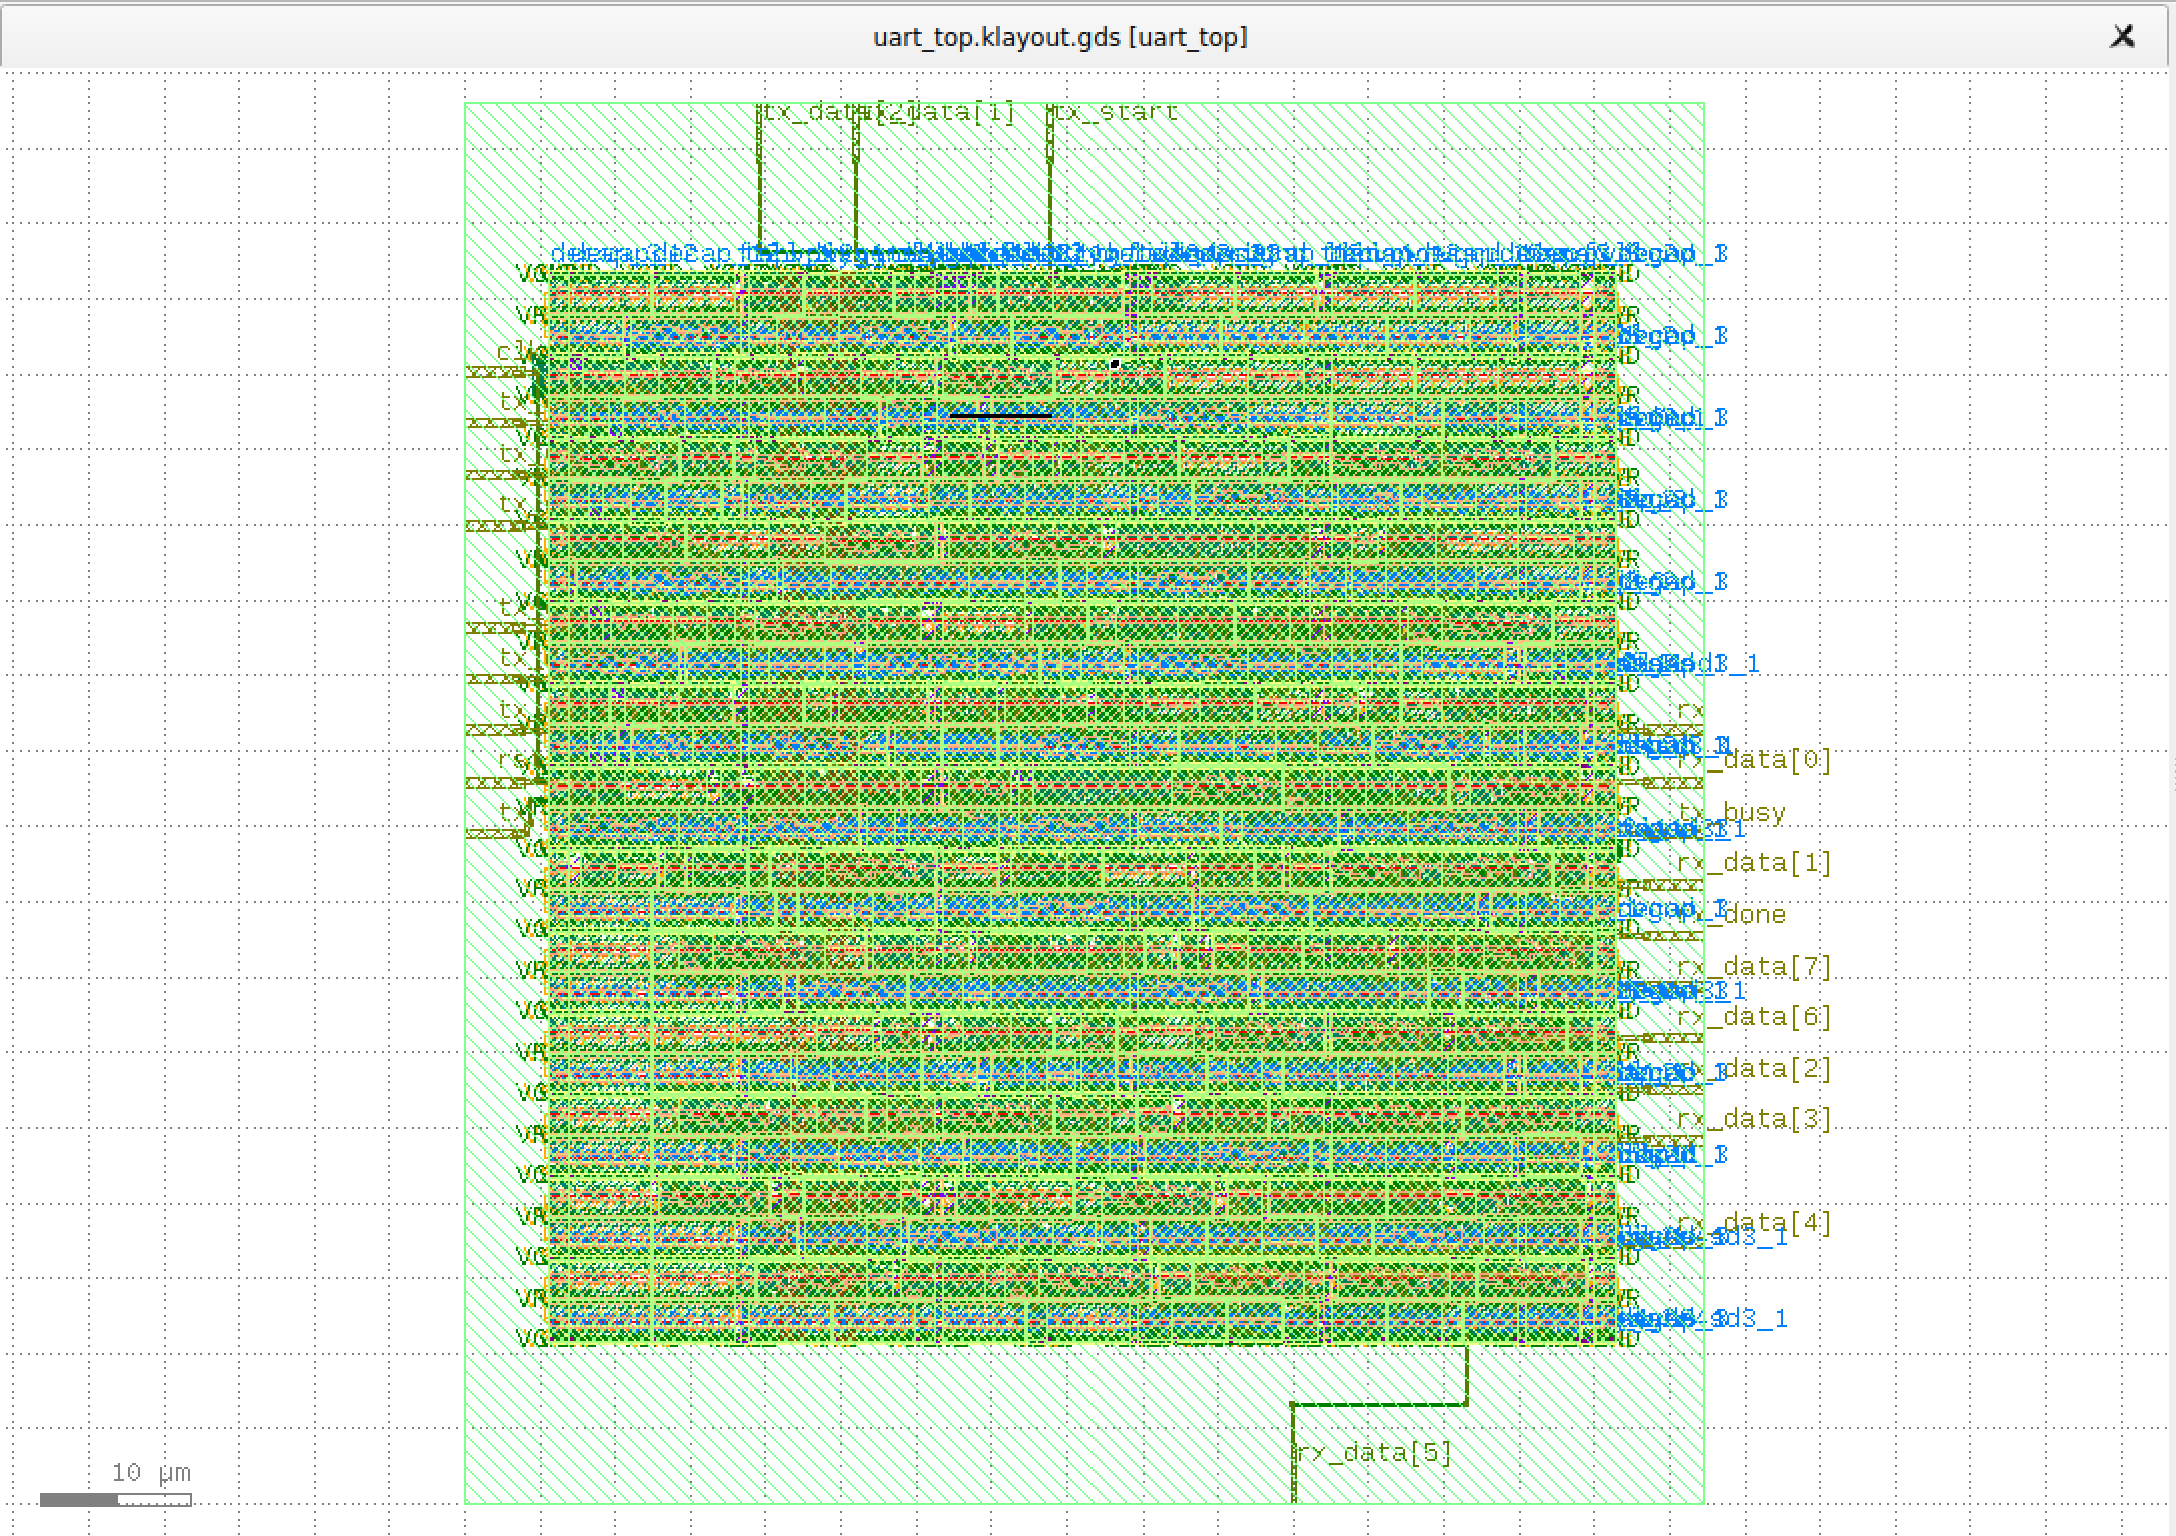
\includegraphics[width=0.92\textwidth]{images/Final_GDSII_Layout_in_KLayout.png}
    \caption{Final GDSII layout of the UART IP core viewed in KLayout.}
    \label{fig:gds_layout}
\end{figure}



\section{Manufacturability Assessment}

The final manufacturability report summarizes the overall fabrication readiness of the design by combining the results of antenna checking, DRC, and LVS verification.


The verification summary is presented in Table~\ref{tab:manufacturability}.

\begin{table}[!htbp]
\centering
\caption{Manufacturability verification summary}
\label{tab:manufacturability}
\begin{tabular}{lc}
\toprule
Verification Stage & Status\\
\midrule
Antenna Check & PASS\\
Magic DRC & PASS\\
Netgen LVS & PASS\\
Manufacturability & PASS\\
\bottomrule
\end{tabular}
\end{table}

The successful completion of all verification stages confirms that the UART ASIC implementation satisfies the required design rules and verification checks. The generated layout is therefore considered suitable for fabrication using the SKY130 process.
\chapter{Results and Discussion}
\label{chap:results and discussion}

This chapter presents the key outcomes obtained during the complete RTL-to-GDSII implementation of the UART IP core. The results include functional verification, synthesis statistics, physical implementation metrics, routing performance, power integrity analysis, physical verification, and the final GDSII layout.

%%%%%%%%%%%%%%%%%%%%%%%%%%%%%%%%%%%%%%%%%%%%%%%%%%%%%%%%%%%%%%%

\section{Functional Verification}

The UART IP core was functionally verified using dedicated Verilog testbenches. The generated simulation waveforms confirm the correct operation of each RTL module before physical implementation.

%%%%%%%%%%%%%%%%%%%%%%%%%%%%%%%%%%%%%%%%%%%%%%%%%%%%%%%%%%%%%%%

\subsection{Baud Rate Generator}

\begin{figure}[!htbp]
\centering
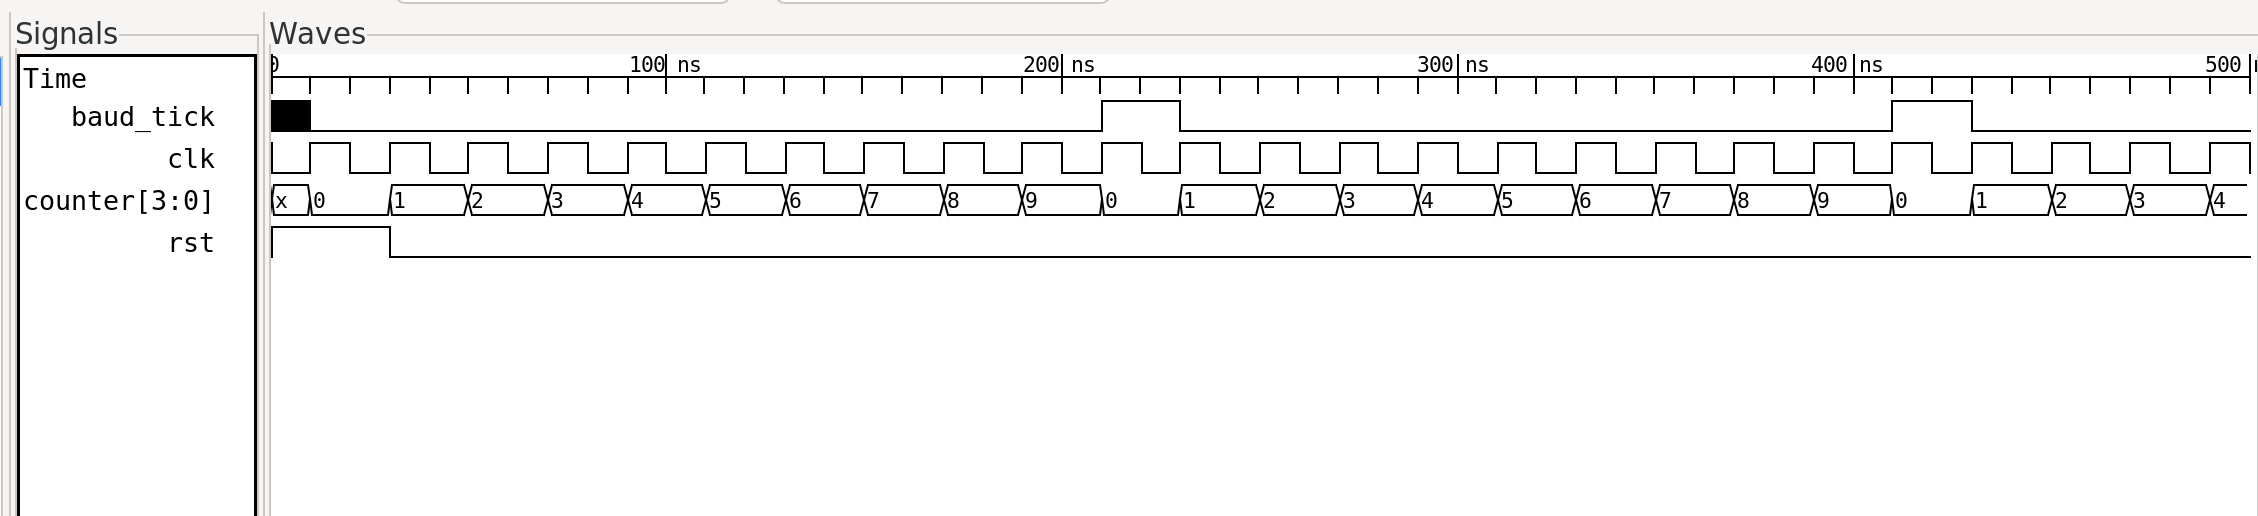
\includegraphics[width=\textwidth]{images/baud_generator_waveform.png}
\caption{Simulation waveform of the Baud Rate Generator.}
\label{fig:baud_wave}
\end{figure}

The waveform verifies that the baud generator correctly divides the system clock and produces periodic baud timing pulses for UART communication.

%%%%%%%%%%%%%%%%%%%%%%%%%%%%%%%%%%%%%%%%%%%%%%%%%%%%%%%%%%%%%%%

\subsection{UART Transmitter}

\begin{figure}[!htbp]
\centering
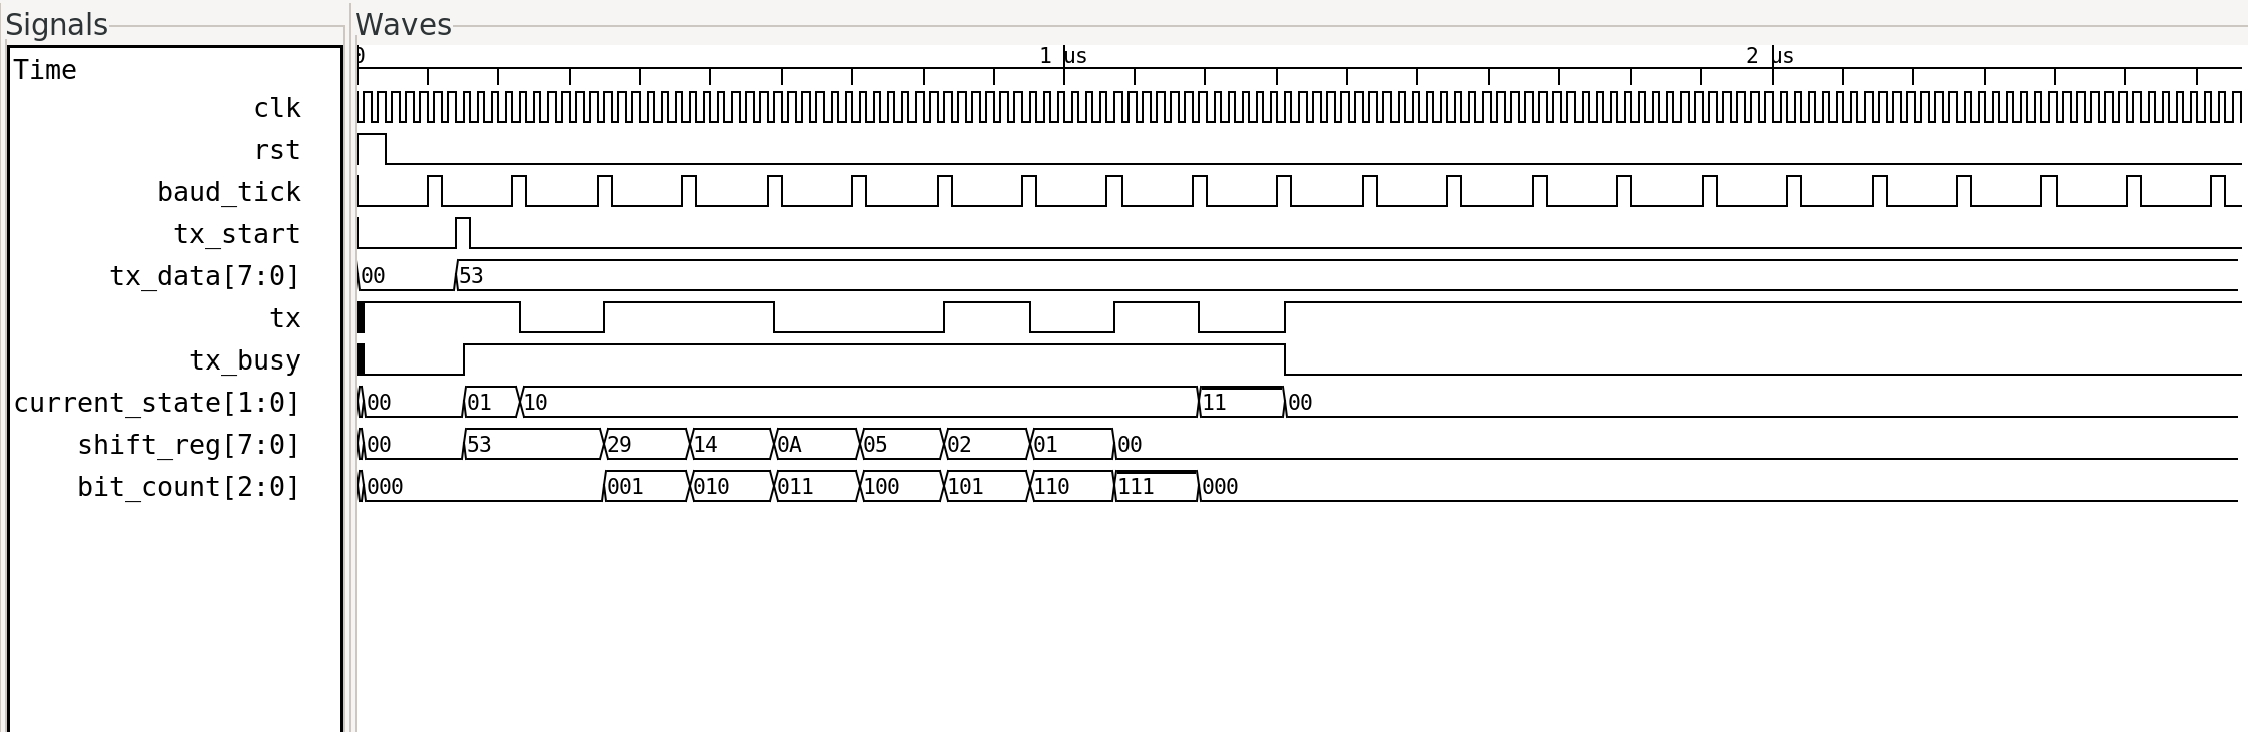
\includegraphics[width=\textwidth]{images/transmitter_waveform.png}
\caption{Simulation waveform of the UART transmitter.}
\label{fig:tx_wave}
\end{figure}

The transmitter correctly generates the UART frame consisting of one start bit, eight data bits, and one stop bit.

%%%%%%%%%%%%%%%%%%%%%%%%%%%%%%%%%%%%%%%%%%%%%%%%%%%%%%%%%%%%%%%

\subsection{UART Receiver}

\begin{figure}[!htbp]
\centering
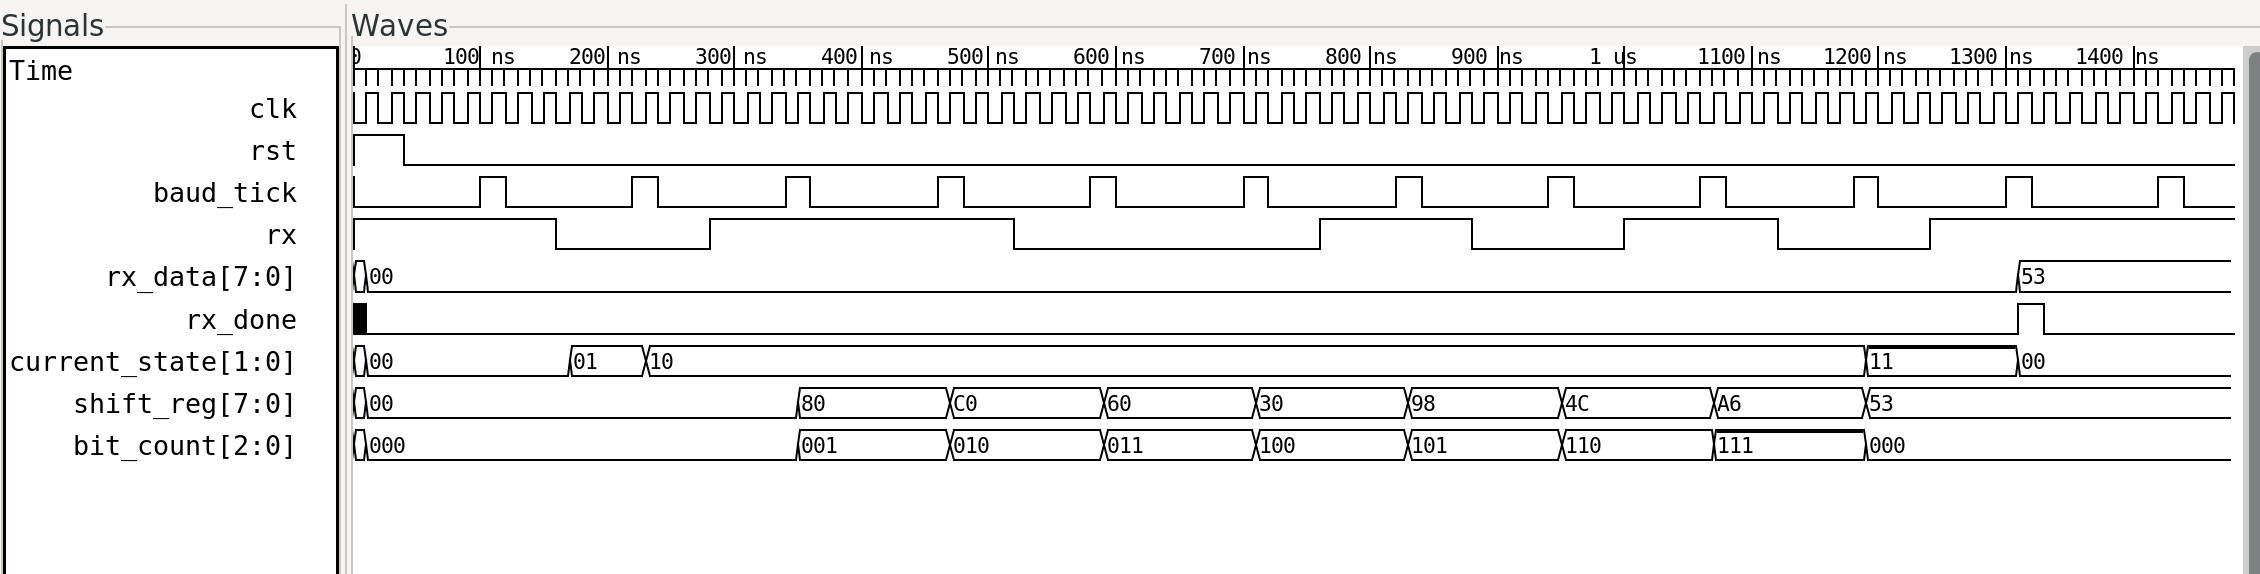
\includegraphics[width=\textwidth]{images/receiver_wavefrom.png}
\caption{Simulation waveform of the UART receiver.}
\label{fig:rx_wave}
\end{figure}

The receiver successfully reconstructs the transmitted serial data and asserts the receive-complete signal after reception.

%%%%%%%%%%%%%%%%%%%%%%%%%%%%%%%%%%%%%%%%%%%%%%%%%%%%%%%%%%%%%%%

\subsection{UART Top Module}

\begin{figure}[!htbp]
\centering
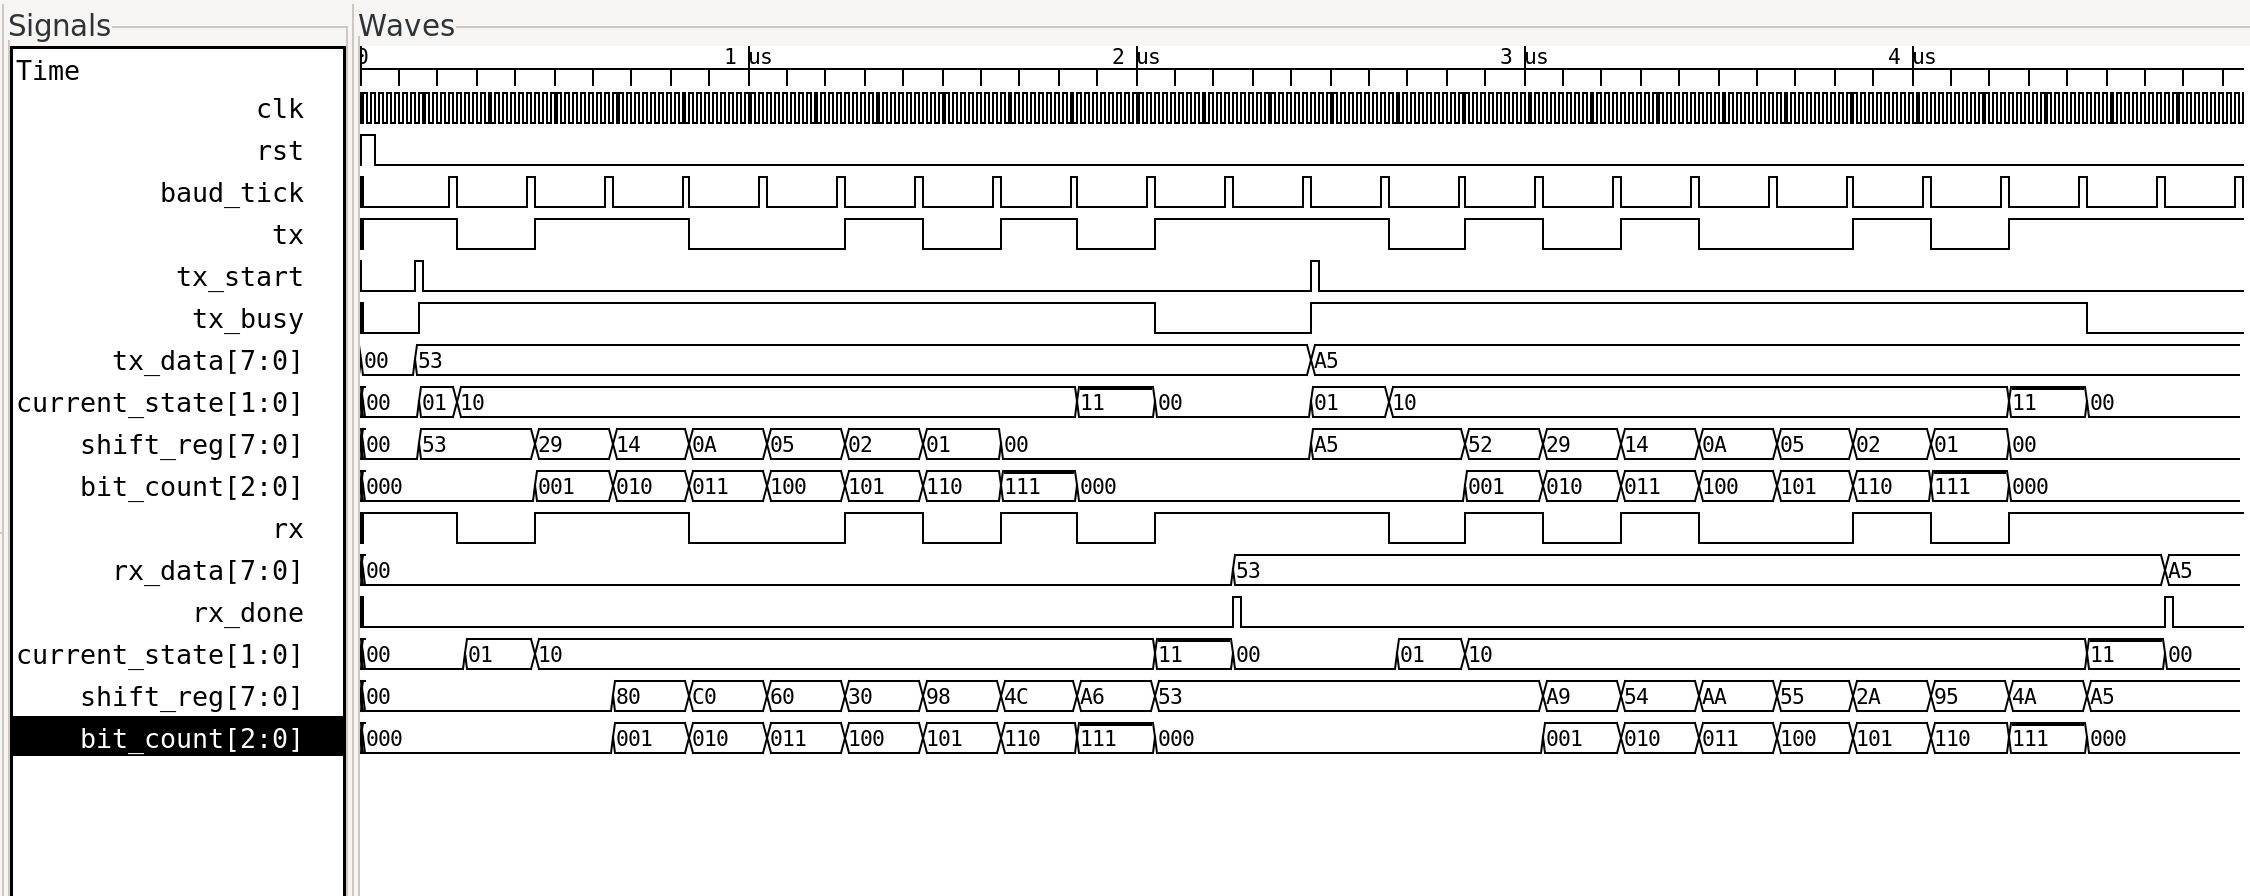
\includegraphics[width=\textwidth]{images/uart_waveform.png}
\caption{Simulation waveform of the complete UART top module.}
\label{fig:top_wave}
\end{figure}

The complete UART system performs successful end-to-end serial communication, confirming proper integration of all RTL modules.

%%%%%%%%%%%%%%%%%%%%%%%%%%%%%%%%%%%%%%%%%%%%%%%%%%%%%%%%%%%%%%%

\section{RTL Synthesis Results}

The RTL was synthesized using Yosys and mapped to the SKY130 standard-cell library.

\begin{table}[!htbp]
\centering
\caption{RTL synthesis summary}
\label{tab:synthesis}
\begin{tabular}{lc}
\toprule
Parameter & Value\\
\midrule
Standard Cells & 219\\
Sequential Cells & 55\\
Cell Area & 2539.936 $\mu m^2$\\
Sequential Area Ratio & 46.06\%\\
Technology Library & SKY130 HD\\
\bottomrule
\end{tabular}
\end{table}

The synthesis completed successfully and generated a technology-mapped gate-level netlist suitable for ASIC implementation.

%%%%%%%%%%%%%%%%%%%%%%%%%%%%%%%%%%%%%%%%%%%%%%%%%%%%%%%%%%%%%%%

\section{Floorplanning Results}

\begin{table}[!htbp]
\centering
\caption{Floorplanning results}
\label{tab:floorplan_result}
\begin{tabular}{lc}
\toprule
Metric & Value\\
\midrule
Die Area & 7658.18 $\mu m^2$\\
Core Area & 5009.80 $\mu m^2$\\
Standard Cell Area & 3210.58 $\mu m^2$\\
Core Utilization & 64.09\%\\
Design Instances & 375\\
I/O Pins & 25\\
\bottomrule
\end{tabular}
\end{table}

The generated floorplan provides sufficient whitespace for routing while maintaining efficient silicon utilization.

%%%%%%%%%%%%%%%%%%%%%%%%%%%%%%%%%%%%%%%%%%%%%%%%%%%%%%%%%%%%%%%

\section{Placement Results}

\begin{table}[!htbp]
\centering
\caption{Placement statistics}
\label{tab:placement_result}
\begin{tabular}{lc}
\toprule
Metric & Value\\
\midrule
HPWL Before Optimization & 3351.5 $\mu m$\\
HPWL After Optimization & 3207.2 $\mu m$\\
HPWL Improvement & 4.3\%\\
Total Displacement & 0 $\mu m$\\
Average Displacement & 0 $\mu m$\\
Maximum Displacement & 0 $\mu m$\\
\bottomrule
\end{tabular}
\end{table}

The placement stage successfully legalized all cells while reducing the estimated routing length.

%%%%%%%%%%%%%%%%%%%%%%%%%%%%%%%%%%%%%%%%%%%%%%%%%%%%%%%%%%%%%%%

\section{Clock Tree Synthesis Results}

\begin{table}[H]
\centering
\caption{CTS statistics}
\label{tab:cts_result}
\begin{tabular}{lc}
\toprule
Metric & Value\\
\midrule
Clock Nets & 6\\
Clock Buffers & 5\\
Clock Inverters & 3\\
Timing Repair Buffers & 78\\
Total Cell Area & 3405.77 $\mu m^2$\\
\bottomrule
\end{tabular}
\end{table}

The generated clock tree provides balanced clock distribution with automatic timing optimization.

%%%%%%%%%%%%%%%%%%%%%%%%%%%%%%%%%%%%%%%%%%%%%%%%%%%%%%%%%%%%%%%

\section{Routing Results}

\begin{table}[!htbp]
\centering
\caption{Routing statistics}
\label{tab:routing_result}
\begin{tabular}{lc}
\toprule
Metric & Value\\
\midrule
Routed Nets & 314\\
Wirelength & 8404 $\mu m$\\
Total Vias & 1804\\
Routing Utilization & 14.71\%\\
Routing Overflow & 0\\
Antenna Violations & 0\\
\bottomrule
\end{tabular}
\end{table}

The routing stage completed successfully with zero congestion overflow and no antenna violations.

%%%%%%%%%%%%%%%%%%%%%%%%%%%%%%%%%%%%%%%%%%%%%%%%%%%%%%%%%%%%%%%

\section{Power Integrity Results}

\begin{table}[!htbp]
\centering
\caption{IR-drop summary}
\label{tab:irdrop_result}
\begin{tabular}{lcc}
\toprule
Parameter & VPWR & VGND\\
\midrule
Worst Voltage & 1.79984 V & 0.000233 V\\
Worst IR Drop & 0.0001605 V & 0.0002330 V\\
Average IR Drop & 0.0000416 V & 0.0000400 V\\
Percentage Drop & 0.01\% & 0.01\%\\
\bottomrule
\end{tabular}
\end{table}

The measured voltage drop is extremely small, indicating a robust power delivery network.

%%%%%%%%%%%%%%%%%%%%%%%%%%%%%%%%%%%%%%%%%%%%%%%%%%%%%%%%%%%%%%%

\section{Physical Verification Results}

\begin{table}[!htbp]
\centering
\caption{Verification summary}
\label{tab:verification}
\begin{tabular}{lc}
\toprule
Verification & Status\\
\midrule
Magic DRC & PASS\\
DRC Violations & 0\\
Netgen LVS & PASS\\
Antenna Check & PASS\\
Manufacturability & PASS\\
\bottomrule
\end{tabular}
\end{table}

All physical verification stages completed successfully, confirming that the generated layout satisfies the SKY130 design rules.

%%%%%%%%%%%%%%%%%%%%%%%%%%%%%%%%%%%%%%%%%%%%%%%%%%%%%%%%%%%%%%%


%%%%%%%%%%%%%%%%%%%%%%%%%%%%%%%%%%%%%%%%%%%%%%%%%%%%%%%%%%%%%%%

\section{Overall Discussion}

The UART IP core was successfully implemented using the complete open-source RTL-to-GDSII design flow. Functional verification confirmed correct UART operation, while physical implementation achieved efficient utilization, successful timing closure, zero routing overflow, negligible IR drop, and clean physical verification results. The final layout passed DRC, LVS, antenna, and manufacturability verification, demonstrating that the generated GDSII layout is suitable for fabrication using the SkyWater SKY130 PDK.
\chapter{Conclusion}
\label{chap:conclusion}

This project successfully demonstrated the complete RTL-to-GDSII implementation of a UART (Universal Asynchronous Receiver-Transmitter) IP core using the open-source OpenLane2 ASIC design flow and the SkyWater SKY130 Process Design Kit (PDK). The UART was designed in Verilog HDL using a modular architecture consisting of a Baud Rate Generator, UART Transmitter, UART Receiver, and a top-level integration module. Functional verification through simulation confirmed the correct operation of each module as well as the complete UART system.

The verified RTL was synthesized using Yosys and subsequently implemented through the OpenROAD physical design flow. The implementation included floorplanning, standard-cell placement, clock tree synthesis, global routing, and detailed routing, resulting in a complete physical layout of the UART IP core. Throughout the implementation process, the design achieved successful placement, balanced clock distribution, congestion-free routing, and efficient utilization of the available routing resources.

Post-layout verification was performed using OpenRCX, OpenSTA, Magic, and Netgen. RC extraction, timing analysis, IR-drop analysis, Design Rule Checking (DRC), Layout Versus Schematic (LVS) verification, and manufacturability assessment were all completed successfully. The generated layout reported zero routing overflow, zero antenna violations, zero DRC violations, successful LVS matching, and negligible IR drop, demonstrating the correctness and fabrication readiness of the design.

Overall, this project provides practical experience with the complete digital ASIC implementation flow using entirely open-source EDA tools. It demonstrates the transformation of a synthesizable RTL design into a verified GDSII layout while exposing every major stage of modern ASIC design, including synthesis, physical implementation, verification, and signoff.

\section*{Future Work}

The current UART IP core can be extended to support additional communication features and more complex System-on-Chip (SoC) designs. Possible future enhancements include:

\begin{itemize}
    \item Configurable baud rates and programmable data formats.
    \item Support for parity generation and parity error detection.
    \item FIFO-based transmit and receive buffers for improved throughput.
    \item Interrupt-driven UART operation for processor-based systems.
    \item Integration with standard on-chip buses such as APB or AXI-Lite.
    \item FPGA prototyping followed by fabrication through an MPW shuttle run.
\end{itemize}


\nocite{*}
\bibliographystyle{IEEEtran}
\bibliography{bibliography/references}

\end{document}
